\documentclass[]{article}
\usepackage{lmodern}
\usepackage{amssymb,amsmath}
\usepackage{ifxetex,ifluatex}
\usepackage{fixltx2e} % provides \textsubscript
\ifnum 0\ifxetex 1\fi\ifluatex 1\fi=0 % if pdftex
  \usepackage[T1]{fontenc}
  \usepackage[utf8]{inputenc}
\else % if luatex or xelatex
  \ifxetex
    \usepackage{mathspec}
  \else
    \usepackage{fontspec}
  \fi
  \defaultfontfeatures{Ligatures=TeX,Scale=MatchLowercase}
\fi
% use upquote if available, for straight quotes in verbatim environments
\IfFileExists{upquote.sty}{\usepackage{upquote}}{}
% use microtype if available
\IfFileExists{microtype.sty}{%
\usepackage{microtype}
\UseMicrotypeSet[protrusion]{basicmath} % disable protrusion for tt fonts
}{}
\usepackage[margin=1in]{geometry}
\usepackage{hyperref}
\hypersetup{unicode=true,
            pdftitle={Week2-Data Management},
            pdfauthor={Matthew Onimus},
            pdfborder={0 0 0},
            breaklinks=true}
\urlstyle{same}  % don't use monospace font for urls
\usepackage{color}
\usepackage{fancyvrb}
\newcommand{\VerbBar}{|}
\newcommand{\VERB}{\Verb[commandchars=\\\{\}]}
\DefineVerbatimEnvironment{Highlighting}{Verbatim}{commandchars=\\\{\}}
% Add ',fontsize=\small' for more characters per line
\usepackage{framed}
\definecolor{shadecolor}{RGB}{248,248,248}
\newenvironment{Shaded}{\begin{snugshade}}{\end{snugshade}}
\newcommand{\AlertTok}[1]{\textcolor[rgb]{0.94,0.16,0.16}{#1}}
\newcommand{\AnnotationTok}[1]{\textcolor[rgb]{0.56,0.35,0.01}{\textbf{\textit{#1}}}}
\newcommand{\AttributeTok}[1]{\textcolor[rgb]{0.77,0.63,0.00}{#1}}
\newcommand{\BaseNTok}[1]{\textcolor[rgb]{0.00,0.00,0.81}{#1}}
\newcommand{\BuiltInTok}[1]{#1}
\newcommand{\CharTok}[1]{\textcolor[rgb]{0.31,0.60,0.02}{#1}}
\newcommand{\CommentTok}[1]{\textcolor[rgb]{0.56,0.35,0.01}{\textit{#1}}}
\newcommand{\CommentVarTok}[1]{\textcolor[rgb]{0.56,0.35,0.01}{\textbf{\textit{#1}}}}
\newcommand{\ConstantTok}[1]{\textcolor[rgb]{0.00,0.00,0.00}{#1}}
\newcommand{\ControlFlowTok}[1]{\textcolor[rgb]{0.13,0.29,0.53}{\textbf{#1}}}
\newcommand{\DataTypeTok}[1]{\textcolor[rgb]{0.13,0.29,0.53}{#1}}
\newcommand{\DecValTok}[1]{\textcolor[rgb]{0.00,0.00,0.81}{#1}}
\newcommand{\DocumentationTok}[1]{\textcolor[rgb]{0.56,0.35,0.01}{\textbf{\textit{#1}}}}
\newcommand{\ErrorTok}[1]{\textcolor[rgb]{0.64,0.00,0.00}{\textbf{#1}}}
\newcommand{\ExtensionTok}[1]{#1}
\newcommand{\FloatTok}[1]{\textcolor[rgb]{0.00,0.00,0.81}{#1}}
\newcommand{\FunctionTok}[1]{\textcolor[rgb]{0.00,0.00,0.00}{#1}}
\newcommand{\ImportTok}[1]{#1}
\newcommand{\InformationTok}[1]{\textcolor[rgb]{0.56,0.35,0.01}{\textbf{\textit{#1}}}}
\newcommand{\KeywordTok}[1]{\textcolor[rgb]{0.13,0.29,0.53}{\textbf{#1}}}
\newcommand{\NormalTok}[1]{#1}
\newcommand{\OperatorTok}[1]{\textcolor[rgb]{0.81,0.36,0.00}{\textbf{#1}}}
\newcommand{\OtherTok}[1]{\textcolor[rgb]{0.56,0.35,0.01}{#1}}
\newcommand{\PreprocessorTok}[1]{\textcolor[rgb]{0.56,0.35,0.01}{\textit{#1}}}
\newcommand{\RegionMarkerTok}[1]{#1}
\newcommand{\SpecialCharTok}[1]{\textcolor[rgb]{0.00,0.00,0.00}{#1}}
\newcommand{\SpecialStringTok}[1]{\textcolor[rgb]{0.31,0.60,0.02}{#1}}
\newcommand{\StringTok}[1]{\textcolor[rgb]{0.31,0.60,0.02}{#1}}
\newcommand{\VariableTok}[1]{\textcolor[rgb]{0.00,0.00,0.00}{#1}}
\newcommand{\VerbatimStringTok}[1]{\textcolor[rgb]{0.31,0.60,0.02}{#1}}
\newcommand{\WarningTok}[1]{\textcolor[rgb]{0.56,0.35,0.01}{\textbf{\textit{#1}}}}
\usepackage{longtable,booktabs}
\usepackage{graphicx,grffile}
\makeatletter
\def\maxwidth{\ifdim\Gin@nat@width>\linewidth\linewidth\else\Gin@nat@width\fi}
\def\maxheight{\ifdim\Gin@nat@height>\textheight\textheight\else\Gin@nat@height\fi}
\makeatother
% Scale images if necessary, so that they will not overflow the page
% margins by default, and it is still possible to overwrite the defaults
% using explicit options in \includegraphics[width, height, ...]{}
\setkeys{Gin}{width=\maxwidth,height=\maxheight,keepaspectratio}
\IfFileExists{parskip.sty}{%
\usepackage{parskip}
}{% else
\setlength{\parindent}{0pt}
\setlength{\parskip}{6pt plus 2pt minus 1pt}
}
\setlength{\emergencystretch}{3em}  % prevent overfull lines
\providecommand{\tightlist}{%
  \setlength{\itemsep}{0pt}\setlength{\parskip}{0pt}}
\setcounter{secnumdepth}{5}
% Redefines (sub)paragraphs to behave more like sections
\ifx\paragraph\undefined\else
\let\oldparagraph\paragraph
\renewcommand{\paragraph}[1]{\oldparagraph{#1}\mbox{}}
\fi
\ifx\subparagraph\undefined\else
\let\oldsubparagraph\subparagraph
\renewcommand{\subparagraph}[1]{\oldsubparagraph{#1}\mbox{}}
\fi

%%% Use protect on footnotes to avoid problems with footnotes in titles
\let\rmarkdownfootnote\footnote%
\def\footnote{\protect\rmarkdownfootnote}

%%% Change title format to be more compact
\usepackage{titling}

% Create subtitle command for use in maketitle
\newcommand{\subtitle}[1]{
  \posttitle{
    \begin{center}\large#1\end{center}
    }
}

\setlength{\droptitle}{-2em}

  \title{Week2-Data Management}
    \pretitle{\vspace{\droptitle}\centering\huge}
  \posttitle{\par}
    \author{Matthew Onimus}
    \preauthor{\centering\large\emph}
  \postauthor{\par}
      \predate{\centering\large\emph}
  \postdate{\par}
    \date{2020-09-17}

\usepackage{amsmath}
\usepackage{booktabs}
\usepackage{caption}
\usepackage{longtable}

\begin{document}
\maketitle

{
\setcounter{tocdepth}{2}
\tableofcontents
}
\begin{Shaded}
\begin{Highlighting}[]
\KeywordTok{library}\NormalTok{(tidyverse)}
\KeywordTok{library}\NormalTok{(gtsummary)}
\KeywordTok{library}\NormalTok{(gt)}
\KeywordTok{library}\NormalTok{(haven)}
\KeywordTok{library}\NormalTok{(readxl)}
\KeywordTok{library}\NormalTok{(rlang)}
\KeywordTok{library}\NormalTok{(corrplot)}
\end{Highlighting}
\end{Shaded}

\hypertarget{reading-in-the-data}{%
\section{Reading in the Data}\label{reading-in-the-data}}

The first thing I needed to do was read the data in join as per the SAS
script.

\begin{Shaded}
\begin{Highlighting}[]
\NormalTok{nhanesdemo <-}\StringTok{ }\KeywordTok{read_sav}\NormalTok{(}\StringTok{"assignments/NHANES_2015_DEMO.sav"}\NormalTok{) }
\NormalTok{nhanesbmx <-}\StringTok{ }\KeywordTok{read_csv}\NormalTok{(}\StringTok{"assignments/NHANES_2015_BMX_I.csv"}\NormalTok{)}
\NormalTok{nhaneshosp <-}\StringTok{ }\KeywordTok{read_excel}\NormalTok{(}\StringTok{"assignments/NHANES_2015_HUQ.xlsx"}\NormalTok{)}

\CommentTok{# note that all the data is not the same legnth}

\NormalTok{nhanes <-}\StringTok{ }\NormalTok{nhanesdemo }\OperatorTok\StringTok{ }
\StringTok{  }\KeywordTok{left_join}\NormalTok{(nhanesbmx, }\DataTypeTok{by =} \StringTok{"SEQN"}\NormalTok{) }\OperatorTok\StringTok{ }
\StringTok{  }\KeywordTok{left_join}\NormalTok{(nhaneshosp, }\DataTypeTok{by =} \StringTok{"SEQN"}\NormalTok{)}

\KeywordTok{tbl_summary}\NormalTok{(nhanes)}
\end{Highlighting}
\end{Shaded}

\begin{longtable}[]{@{}ll@{}}
\toprule
\textbf{Characteristic} & \textbf{N = 9,971}\tabularnewline
\midrule
\endhead
Respondent sequence number & 88,717 (86,224, 91,210)\tabularnewline
Data release cycle &\tabularnewline
9 & 9,971 (100\%)\tabularnewline
Interview/Examination status &\tabularnewline
1 & 427 (4.3\%)\tabularnewline
2 & 9,544 (96\%)\tabularnewline
Gender &\tabularnewline
1 & 4,892 (49\%)\tabularnewline
2 & 5,079 (51\%)\tabularnewline
Age in years at screening & 27 (9, 53)\tabularnewline
Age in months at screening - 0 to 24 mos & 10 (5, 17)\tabularnewline
Unknown & 9,276\tabularnewline
Race/Hispanic origin &\tabularnewline
1 & 1,921 (19\%)\tabularnewline
2 & 1,308 (13\%)\tabularnewline
3 & 3,066 (31\%)\tabularnewline
4 & 2,129 (21\%)\tabularnewline
5 & 1,547 (16\%)\tabularnewline
Race/Hispanic origin w/ NH Asian &\tabularnewline
1 & 1,921 (19\%)\tabularnewline
2 & 1,308 (13\%)\tabularnewline
3 & 3,066 (31\%)\tabularnewline
4 & 2,129 (21\%)\tabularnewline
6 & 1,042 (10\%)\tabularnewline
7 & 505 (5.1\%)\tabularnewline
Six month time period &\tabularnewline
1 & 4,594 (48\%)\tabularnewline
2 & 4,950 (52\%)\tabularnewline
Unknown & 427\tabularnewline
Age in months at exam - 0 to 19 years & 100 (41, 162)\tabularnewline
Unknown & 5,911\tabularnewline
Served active duty in US Armed Forces &\tabularnewline
1 & 527 (8.6\%)\tabularnewline
2 & 5,622 (91\%)\tabularnewline
Unknown & 3,822\tabularnewline
Served in a foreign country &\tabularnewline
1 & 258 (49\%)\tabularnewline
2 & 267 (51\%)\tabularnewline
7 & 2 (0.4\%)\tabularnewline
Unknown & 9,444\tabularnewline
Country of birth &\tabularnewline
1 & 7,733 (78\%)\tabularnewline
2 & 2,236 (22\%)\tabularnewline
99 & 2 (\textless0.1\%)\tabularnewline
Citizenship status &\tabularnewline
1 & 8,785 (88\%)\tabularnewline
2 & 1,168 (12\%)\tabularnewline
7 & 9 (\textless0.1\%)\tabularnewline
9 & 7 (\textless0.1\%)\tabularnewline
Unknown & 2\tabularnewline
Length of time in US & 5.00 (3.00, 7.00)\tabularnewline
Unknown & 7,735\tabularnewline
Education level - Children/Youth 6-19 & 5.0 (2.0, 9.0)\tabularnewline
Unknown & 7,324\tabularnewline
Education level - Adults 20+ &\tabularnewline
1 & 688 (12\%)\tabularnewline
2 & 676 (12\%)\tabularnewline
3 & 1,236 (22\%)\tabularnewline
4 & 1,692 (30\%)\tabularnewline
5 & 1,422 (25\%)\tabularnewline
9 & 5 (\textless0.1\%)\tabularnewline
Unknown & 4,252\tabularnewline
Marital status &\tabularnewline
1 & 2,886 (50\%)\tabularnewline
2 & 421 (7.4\%)\tabularnewline
3 & 614 (11\%)\tabularnewline
4 & 192 (3.4\%)\tabularnewline
5 & 1,048 (18\%)\tabularnewline
6 & 555 (9.7\%)\tabularnewline
77 & 2 (\textless0.1\%)\tabularnewline
99 & 1 (\textless0.1\%)\tabularnewline
Unknown & 4,252\tabularnewline
Pregnancy status at exam &\tabularnewline
1 & 70 (5.4\%)\tabularnewline
2 & 1,125 (87\%)\tabularnewline
3 & 93 (7.2\%)\tabularnewline
Unknown & 8,683\tabularnewline
Language of SP Interview &\tabularnewline
1 & 8,584 (86\%)\tabularnewline
2 & 1,387 (14\%)\tabularnewline
Proxy used in SP Interview? &\tabularnewline
1 & 3,689 (37\%)\tabularnewline
2 & 6,281 (63\%)\tabularnewline
Unknown & 1\tabularnewline
Interpreter used in SP Interview? &\tabularnewline
1 & 457 (4.6\%)\tabularnewline
2 & 9,514 (95\%)\tabularnewline
Language of Family Interview &\tabularnewline
1 & 8,430 (87\%)\tabularnewline
2 & 1,212 (13\%)\tabularnewline
Unknown & 329\tabularnewline
Proxy used in Family Interview? &\tabularnewline
1 & 9 (\textless0.1\%)\tabularnewline
2 & 9,633 (100\%)\tabularnewline
Unknown & 329\tabularnewline
Interpreter used in Family Interview? &\tabularnewline
1 & 405 (4.2\%)\tabularnewline
2 & 9,237 (96\%)\tabularnewline
Unknown & 329\tabularnewline
Language of MEC Interview &\tabularnewline
1 & 6,382 (91\%)\tabularnewline
2 & 595 (8.5\%)\tabularnewline
Unknown & 2,994\tabularnewline
Proxy used in MEC Interview? &\tabularnewline
1 & 57 (0.8\%)\tabularnewline
2 & 6,921 (99\%)\tabularnewline
Unknown & 2,993\tabularnewline
Interpreter used in MEC Interview? &\tabularnewline
1 & 346 (5.0\%)\tabularnewline
2 & 6,632 (95\%)\tabularnewline
Unknown & 2,993\tabularnewline
Language of ACASI Interview &\tabularnewline
1 & 5,218 (88\%)\tabularnewline
2 & 638 (11\%)\tabularnewline
3 & 106 (1.8\%)\tabularnewline
Unknown & 4,009\tabularnewline
Total number of people in the Household &\tabularnewline
1 & 828 (8.3\%)\tabularnewline
2 & 1,723 (17\%)\tabularnewline
3 & 1,719 (17\%)\tabularnewline
4 & 2,061 (21\%)\tabularnewline
5 & 1,672 (17\%)\tabularnewline
6 & 994 (10.0\%)\tabularnewline
7 & 974 (9.8\%)\tabularnewline
Total number of people in the Family &\tabularnewline
1 & 1,305 (13\%)\tabularnewline
2 & 1,510 (15\%)\tabularnewline
3 & 1,634 (16\%)\tabularnewline
4 & 2,011 (20\%)\tabularnewline
5 & 1,635 (16\%)\tabularnewline
6 & 961 (9.6\%)\tabularnewline
7 & 915 (9.2\%)\tabularnewline
\# of children 5 years or younger in HH &\tabularnewline
0 & 6,298 (63\%)\tabularnewline
1 & 2,147 (22\%)\tabularnewline
2 & 1,199 (12\%)\tabularnewline
3 & 327 (3.3\%)\tabularnewline
\# of children 6-17 years old in HH &\tabularnewline
0 & 4,715 (47\%)\tabularnewline
1 & 1,990 (20\%)\tabularnewline
2 & 1,833 (18\%)\tabularnewline
3 & 822 (8.2\%)\tabularnewline
4 & 611 (6.1\%)\tabularnewline
\# of adults 60 years or older in HH &\tabularnewline
0 & 7,151 (72\%)\tabularnewline
1 & 1,663 (17\%)\tabularnewline
2 & 1,099 (11\%)\tabularnewline
3 & 58 (0.6\%)\tabularnewline
HH ref person's gender &\tabularnewline
1 & 5,053 (51\%)\tabularnewline
2 & 4,918 (49\%)\tabularnewline
HH ref person's age in years & 44 (34, 57)\tabularnewline
HH ref person's country of birth &\tabularnewline
1 & 6,359 (66\%)\tabularnewline
2 & 3,207 (33\%)\tabularnewline
77 & 5 (\textless0.1\%)\tabularnewline
99 & 4 (\textless0.1\%)\tabularnewline
Unknown & 396\tabularnewline
HH ref person's education level &\tabularnewline
1 & 1,087 (11\%)\tabularnewline
2 & 1,200 (13\%)\tabularnewline
3 & 2,015 (21\%)\tabularnewline
4 & 2,908 (30\%)\tabularnewline
5 & 2,331 (24\%)\tabularnewline
9 & 34 (0.4\%)\tabularnewline
Unknown & 396\tabularnewline
HH ref person's marital status &\tabularnewline
1 & 5,681 (57\%)\tabularnewline
2 & 524 (5.3\%)\tabularnewline
3 & 977 (9.9\%)\tabularnewline
4 & 353 (3.6\%)\tabularnewline
5 & 1,305 (13\%)\tabularnewline
6 & 1,017 (10\%)\tabularnewline
77 & 44 (0.4\%)\tabularnewline
99 & 8 (\textless0.1\%)\tabularnewline
Unknown & 62\tabularnewline
HH ref person's spouse's education level &\tabularnewline
1 & 619 (12\%)\tabularnewline
2 & 511 (9.8\%)\tabularnewline
3 & 980 (19\%)\tabularnewline
4 & 1,462 (28\%)\tabularnewline
5 & 1,629 (31\%)\tabularnewline
7 & 2 (\textless0.1\%)\tabularnewline
9 & 23 (0.4\%)\tabularnewline
Unknown & 4,745\tabularnewline
Full sample 2 year interview weight & 20,160 (12,879,
33,257)\tabularnewline
Full sample 2 year MEC exam weight & 20,281 (12,551,
33,708)\tabularnewline
Masked variance pseudo-PSU &\tabularnewline
1 & 5,127 (51\%)\tabularnewline
2 & 4,844 (49\%)\tabularnewline
Masked variance pseudo-stratum & 126.0 (123.0, 130.0)\tabularnewline
Annual household income & 8.0 (6.0, 14.0)\tabularnewline
Unknown & 345\tabularnewline
Annual family income & 8.0 (5.0, 14.0)\tabularnewline
Unknown & 329\tabularnewline
Ratio of family income to poverty & 1.82 (0.97, 3.48)\tabularnewline
Unknown & 1,052\tabularnewline
BMDSTATS &\tabularnewline
1 & 8,687 (91\%)\tabularnewline
2 & 366 (3.8\%)\tabularnewline
3 & 411 (4.3\%)\tabularnewline
4 & 80 (0.8\%)\tabularnewline
Unknown & 427\tabularnewline
BMXWT & 65 (37, 84)\tabularnewline
Unknown & 526\tabularnewline
BMIWT &\tabularnewline
1 & 14 (3.2\%)\tabularnewline
3 & 406 (92\%)\tabularnewline
4 & 23 (5.2\%)\tabularnewline
Unknown & 9,528\tabularnewline
BMXRECUM & 82 (70, 93)\tabularnewline
Unknown & 8,898\tabularnewline
BMIRECUM & 33 (100\%)\tabularnewline
Unknown & 9,938\tabularnewline
BMXHEAD & 41.70 (39.70, 43.20)\tabularnewline
Unknown & 9,756\tabularnewline
BMIHEAD & 0 (NA\%)\tabularnewline
Unknown & 9,971\tabularnewline
BMXHT & 161 (149, 170)\tabularnewline
Unknown & 1,202\tabularnewline
BMIHT &\tabularnewline
1 & 37 (35\%)\tabularnewline
3 & 68 (65\%)\tabularnewline
Unknown & 9,866\tabularnewline
BMXBMI & 25 (20, 31)\tabularnewline
Unknown & 1,215\tabularnewline
BMDBMIC &\tabularnewline
1 & 86 (2.6\%)\tabularnewline
2 & 2,041 (61\%)\tabularnewline
3 & 561 (17\%)\tabularnewline
4 & 652 (20\%)\tabularnewline
Unknown & 6,631\tabularnewline
BMXLEG & 38.2 (35.3, 41.0)\tabularnewline
Unknown & 2,861\tabularnewline
BMILEG & 402 (100\%)\tabularnewline
Unknown & 9,569\tabularnewline
BMXARML & 36 (30, 38)\tabularnewline
Unknown & 995\tabularnewline
BMIARML & 420 (100\%)\tabularnewline
Unknown & 9,551\tabularnewline
BMXARMC & 30 (22, 34)\tabularnewline
Unknown & 995\tabularnewline
BMIARMC & 421 (100\%)\tabularnewline
Unknown & 9,550\tabularnewline
BMXWAIST & 89 (72, 104)\tabularnewline
Unknown & 1,658\tabularnewline
BMIWAIST & 489 (100\%)\tabularnewline
Unknown & 9,482\tabularnewline
BMXSAD1 & 20.9 (17.5, 24.6)\tabularnewline
Unknown & 2,988\tabularnewline
BMXSAD2 & 20.9 (17.5, 24.6)\tabularnewline
Unknown & 2,988\tabularnewline
BMXSAD3 & 22.4 (19.2, 25.9)\tabularnewline
Unknown & 9,618\tabularnewline
BMXSAD4 & 22.7 (19.3, 26.0)\tabularnewline
Unknown & 9,618\tabularnewline
BMDAVSAD & 20.9 (17.5, 24.6)\tabularnewline
Unknown & 2,988\tabularnewline
BMDSADCM &\tabularnewline
1 & 436 (98\%)\tabularnewline
2 & 2 (0.4\%)\tabularnewline
3 & 3 (0.7\%)\tabularnewline
4 & 1 (0.2\%)\tabularnewline
5 & 4 (0.9\%)\tabularnewline
Unknown & 9,525\tabularnewline
HUQ010 &\tabularnewline
1 & 2,561 (26\%)\tabularnewline
2 & 2,658 (27\%)\tabularnewline
3 & 3,001 (30\%)\tabularnewline
4 & 1,424 (14\%)\tabularnewline
5 & 317 (3.2\%)\tabularnewline
7 & 3 (\textless0.1\%)\tabularnewline
9 & 7 (\textless0.1\%)\tabularnewline
HUQ020 &\tabularnewline
1 & 1,965 (21\%)\tabularnewline
2 & 653 (6.8\%)\tabularnewline
3 & 6,954 (73\%)\tabularnewline
9 & 3 (\textless0.1\%)\tabularnewline
Unknown & 396\tabularnewline
HUQ030 &\tabularnewline
1 & 8,563 (86\%)\tabularnewline
2 & 1,340 (13\%)\tabularnewline
3 & 68 (0.7\%)\tabularnewline
HUQ041 &\tabularnewline
1 & 2,979 (35\%)\tabularnewline
2 & 5,093 (59\%)\tabularnewline
3 & 277 (3.2\%)\tabularnewline
4 & 148 (1.7\%)\tabularnewline
5 & 104 (1.2\%)\tabularnewline
6 & 30 (0.3\%)\tabularnewline
Unknown & 1,340\tabularnewline
HUQ051 & 2.00 (1.00, 3.00)\tabularnewline
HUQ061 &\tabularnewline
1 & 114 (8.0\%)\tabularnewline
2 & 104 (7.3\%)\tabularnewline
3 & 508 (36\%)\tabularnewline
4 & 409 (29\%)\tabularnewline
5 & 221 (16\%)\tabularnewline
6 & 59 (4.2\%)\tabularnewline
99 & 6 (0.4\%)\tabularnewline
Unknown & 8,550\tabularnewline
HUQ071 &\tabularnewline
1 & 869 (8.7\%)\tabularnewline
2 & 9,098 (91\%)\tabularnewline
9 & 4 (\textless0.1\%)\tabularnewline
HUD080 &\tabularnewline
1 & 630 (72\%)\tabularnewline
2 & 141 (16\%)\tabularnewline
3 & 55 (6.3\%)\tabularnewline
4 & 18 (2.1\%)\tabularnewline
5 & 14 (1.6\%)\tabularnewline
6 & 10 (1.2\%)\tabularnewline
99999 & 1 (0.1\%)\tabularnewline
Unknown & 9,102\tabularnewline
HUQ090 &\tabularnewline
1 & 788 (9.0\%)\tabularnewline
2 & 8,000 (91\%)\tabularnewline
9 & 6 (\textless0.1\%)\tabularnewline
Unknown & 1,177\tabularnewline
\bottomrule
\end{longtable}

The final, joined data had 81 variables and 9971 observations. A pretty
massive dataset.

\hypertarget{review-the-frequency-table-for-the-number-of-overnight-hospital-visits-and-a-histogram-what-is-this-data-and-distribution-telling-you}{%
\subsection{1. Review the frequency table for the number of overnight
hospital visits and a histogram, what is this data and distribution
telling
you?}\label{review-the-frequency-table-for-the-number-of-overnight-hospital-visits-and-a-histogram-what-is-this-data-and-distribution-telling-you}}

\begin{Shaded}
\begin{Highlighting}[]
\NormalTok{nhanes2 <-}\StringTok{ }\NormalTok{nhanes }\OperatorTok
\StringTok{  }\CommentTok{#select(HUD080, HUQ071) %>% }
\StringTok{  }\KeywordTok{mutate}\NormalTok{(}\DataTypeTok{overnightHosp =}\NormalTok{ HUD080,}
         \DataTypeTok{overnightHosp =} \KeywordTok{ifelse}\NormalTok{(HUQ071}\OperatorTok{==}\DecValTok{7} \OperatorTok{|}\StringTok{ }\NormalTok{HUQ071}\OperatorTok{==}\DecValTok{9} \OperatorTok{|}\StringTok{ }\KeywordTok{is.na}\NormalTok{(HUQ071), }\OtherTok{NA}\NormalTok{, overnightHosp),}
         \DataTypeTok{overnightHosp =} \KeywordTok{ifelse}\NormalTok{(HUQ071 }\OperatorTok{==}\StringTok{ }\DecValTok{1} \OperatorTok{&}\StringTok{ }\NormalTok{(HUD080 }\OperatorTok{==}\StringTok{ }\DecValTok{77777} \OperatorTok{|}\StringTok{ }\NormalTok{HUD080 }\OperatorTok{==}\StringTok{ }\DecValTok{99999}\NormalTok{), }\OtherTok{NA}\NormalTok{, overnightHosp),}
         \DataTypeTok{overnightHosp =} \KeywordTok{ifelse}\NormalTok{(HUQ071 }\OperatorTok{==}\StringTok{ }\DecValTok{2}\NormalTok{, }\DecValTok{0}\NormalTok{, overnightHosp),}
         \DataTypeTok{waistin =}\NormalTok{ BMXWAIST }\OperatorTok{/}\StringTok{ }\FloatTok{2.54}\NormalTok{,}
         \DataTypeTok{children =} \DecValTok{0}\NormalTok{,}
         \DataTypeTok{children =} \KeywordTok{ifelse}\NormalTok{(DMDHHSZA }\OperatorTok{>}\StringTok{ }\DecValTok{0} \OperatorTok{|}\StringTok{ }\NormalTok{DMDHHSZB }\OperatorTok{>}\StringTok{ }\DecValTok{0}\NormalTok{, }\DecValTok{1}\NormalTok{, children)}
         
\NormalTok{  ) }

\NormalTok{nhanesChildren <-}\StringTok{ }\NormalTok{nhanes2 }\OperatorTok\StringTok{ }
\StringTok{  }\KeywordTok{filter}\NormalTok{(children }\OperatorTok{==}\StringTok{ }\DecValTok{1}\NormalTok{)}

\NormalTok{nhanes2 }\OperatorTok\StringTok{ }
\StringTok{  }\KeywordTok{select}\NormalTok{(overnightHosp) }\OperatorTok\StringTok{ }
\StringTok{  }\KeywordTok{group_by}\NormalTok{(overnightHosp) }\OperatorTok\StringTok{ }
\StringTok{  }\KeywordTok{summarise}\NormalTok{(}\DataTypeTok{count =} \KeywordTok{n}\NormalTok{()) }\OperatorTok\StringTok{ }
\StringTok{  }\KeywordTok{gt}\NormalTok{()}
\end{Highlighting}
\end{Shaded}

\captionsetup[table]{labelformat=empty,skip=1pt}
\begin{longtable}{rc}
\toprule
overnightHosp & count \\ 
\midrule
0 & 9098 \\ 
1 & 630 \\ 
2 & 141 \\ 
3 & 55 \\ 
4 & 18 \\ 
5 & 14 \\ 
6 & 10 \\ 
NA & 5 \\ 
\bottomrule
\end{longtable}

\begin{Shaded}
\begin{Highlighting}[]
\KeywordTok{ggplot}\NormalTok{(nhanes2, }\KeywordTok{aes}\NormalTok{(}\DataTypeTok{x =}\NormalTok{ overnightHosp)) }\OperatorTok{+}
\StringTok{  }\KeywordTok{geom_histogram}\NormalTok{(}\DataTypeTok{bins =} \DecValTok{7}\NormalTok{) }\OperatorTok{+}
\StringTok{  }\KeywordTok{theme_classic}\NormalTok{()}
\end{Highlighting}
\end{Shaded}

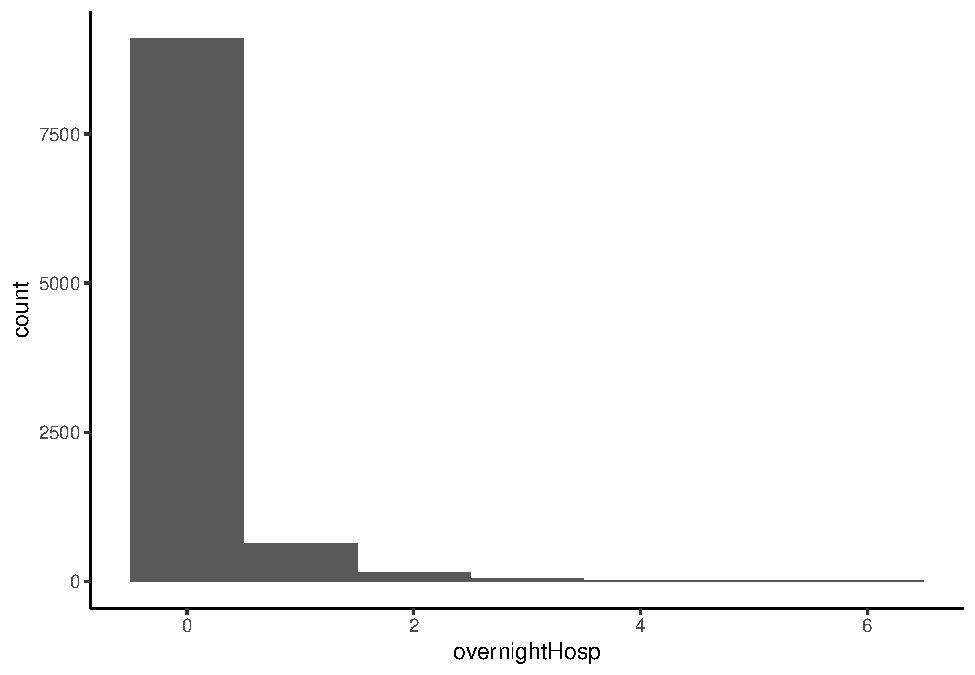
\includegraphics{assignment2_files/figure-latex/q1_hist-1.pdf}

The frequency table shows most of the data do not have an overnight
hospital stay. The histogram tells the same story. There is a large tail
to the data showing the skewness.

\hypertarget{what-is-the-median-age-of-respondents-what-are-the-median-ages-for-those-who-do-and-do-not-have-a-child-in-the-home}{%
\subsection{2. What is the median age of respondents? What are the
median ages for those who do and do not have a child in the
home?}\label{what-is-the-median-age-of-respondents-what-are-the-median-ages-for-those-who-do-and-do-not-have-a-child-in-the-home}}

\begin{Shaded}
\begin{Highlighting}[]
\KeywordTok{median}\NormalTok{(nhanes2}\OperatorTok{$}\NormalTok{RIDAGEYR)}
\end{Highlighting}
\end{Shaded}

\begin{verbatim}
## [1] 27
\end{verbatim}

\begin{Shaded}
\begin{Highlighting}[]
\NormalTok{nhanes2 }\OperatorTok\StringTok{ }
\StringTok{  }\KeywordTok{group_by}\NormalTok{(children) }\OperatorTok\StringTok{ }
\StringTok{  }\KeywordTok{summarise}\NormalTok{(}\DataTypeTok{count =} \KeywordTok{n}\NormalTok{(),}
            \DataTypeTok{median =} \KeywordTok{median}\NormalTok{(RIDAGEYR))}
\end{Highlighting}
\end{Shaded}

\begin{verbatim}
## # A tibble: 2 x 3
##   children count median
##      <dbl> <int>  <dbl>
## 1        0  3330     59
## 2        1  6641     14
\end{verbatim}

The median age for all respondents is 27. The median age for those with
children is 14 and without children is 59.

\hypertarget{what-is-the-average-waist-circumference-in-inches-for-those-who-had-6-overnight-hospital-stays-in-the-past-year}{%
\subsection{3. What is the average waist circumference (in inches) for
those who had 6+ overnight hospital stays in the past
year?}\label{what-is-the-average-waist-circumference-in-inches-for-those-who-had-6-overnight-hospital-stays-in-the-past-year}}

\begin{Shaded}
\begin{Highlighting}[]
\NormalTok{nhanes2 }\OperatorTok\StringTok{ }
\StringTok{  }\KeywordTok{group_by}\NormalTok{(overnightHosp) }\OperatorTok\StringTok{ }
\StringTok{  }\KeywordTok{summarize}\NormalTok{(}\DataTypeTok{count =} \KeywordTok{n}\NormalTok{(),}
            \DataTypeTok{waist =} \KeywordTok{mean}\NormalTok{(waistin, }\DataTypeTok{na.rm =} \OtherTok{TRUE}\NormalTok{)) }\OperatorTok\StringTok{ }
\StringTok{  }\KeywordTok{gt}\NormalTok{()}
\end{Highlighting}
\end{Shaded}

\captionsetup[table]{labelformat=empty,skip=1pt}
\begin{longtable}{rcr}
\toprule
overnightHosp & count & waist \\ 
\midrule
0 & 9098 & 34.30683 \\ 
1 & 630 & 38.39725 \\ 
2 & 141 & 40.62992 \\ 
3 & 55 & 39.03864 \\ 
4 & 18 & 39.01247 \\ 
5 & 14 & 34.54068 \\ 
6 & 10 & 36.84055 \\ 
NA & 5 & 35.27559 \\ 
\bottomrule
\end{longtable}

The average waist size (in inches) for 6 overnight stays is 36.841
inches.

\hypertarget{create-a-cross-tabulation-for-the-number-of-overnight-hospital-stays-with-raceethnicity-ridreth3.-which-group-had-the-lowest-proportion-on-inpatients-the-greatest-proportion-of-high-utilizers}{%
\subsection{4. Create a cross-tabulation for the number of overnight
hospital stays with race/ethnicity (RIDRETH3). Which group had the
lowest proportion on inpatients? The greatest proportion of high
utilizers?}\label{create-a-cross-tabulation-for-the-number-of-overnight-hospital-stays-with-raceethnicity-ridreth3.-which-group-had-the-lowest-proportion-on-inpatients-the-greatest-proportion-of-high-utilizers}}

\begin{Shaded}
\begin{Highlighting}[]
\NormalTok{nhanes2 }\OperatorTok\StringTok{ }
\StringTok{  }\KeywordTok{select}\NormalTok{(overnightHosp, RIDRETH3) }\OperatorTok\StringTok{ }
\StringTok{  }\KeywordTok{tbl_summary}\NormalTok{(}\DataTypeTok{by =}\NormalTok{ RIDRETH3, }\DataTypeTok{percent =} \StringTok{'cell'}\NormalTok{) }\OperatorTok\StringTok{ }
\StringTok{  }\KeywordTok{add_overall}\NormalTok{() }\OperatorTok\StringTok{ }
\StringTok{  }\KeywordTok{as_gt}\NormalTok{() }\OperatorTok\StringTok{ }
\StringTok{  }\CommentTok{#tab_header(title = "Table of overnighthosp by RIDRETH3") %>% }
\StringTok{  }\KeywordTok{tab_spanner}\NormalTok{(}\DataTypeTok{label =} \StringTok{"RIDRETH3(Race/Hispanic origin w/ NH Asian)"}\NormalTok{, }\DataTypeTok{columns =} \KeywordTok{c}\NormalTok{(}\DecValTok{5}\OperatorTok{:}\DecValTok{10}\NormalTok{))}
\end{Highlighting}
\end{Shaded}

\captionsetup[table]{labelformat=empty,skip=1pt}
\begin{longtable}{lccccccc}
\toprule
& & \multicolumn{6}{c}{RIDRETH3(Race/Hispanic origin w/ NH Asian)} \\ 
 \cmidrule(lr){3-8}
\textbf{Characteristic} & \textbf{Overall}, N = 9,971 & \textbf{1}, N = 1,921\textsuperscript{1} & \textbf{2}, N = 1,308\textsuperscript{1} & \textbf{3}, N = 3,066\textsuperscript{1} & \textbf{4}, N = 2,129\textsuperscript{1} & \textbf{6}, N = 1,042\textsuperscript{1} & \textbf{7}, N = 505\textsuperscript{1} \\ 
\midrule
overnightHosp &  &  &  &  &  &  &  \\ 
0 & 9,098 (91\%) & 1,782 (18\%) & 1,178 (12\%) & 2,802 (28\%) & 1,909 (19\%) & 981 (9.8\%) & 446 (4.5\%) \\ 
1 & 630 (6.3\%) & 103 (1.0\%) & 93 (0.9\%) & 194 (1.9\%) & 153 (1.5\%) & 46 (0.5\%) & 41 (0.4\%) \\ 
2 & 141 (1.4\%) & 24 (0.2\%) & 21 (0.2\%) & 44 (0.4\%) & 35 (0.4\%) & 10 (0.1\%) & 7 (<0.1\%) \\ 
3 & 55 (0.6\%) & 6 (<0.1\%) & 9 (<0.1\%) & 12 (0.1\%) & 21 (0.2\%) & 3 (<0.1\%) & 4 (<0.1\%) \\ 
4 & 18 (0.2\%) & 1 (<0.1\%) & 4 (<0.1\%) & 6 (<0.1\%) & 4 (<0.1\%) & 1 (<0.1\%) & 2 (<0.1\%) \\ 
5 & 14 (0.1\%) & 2 (<0.1\%) & 0 (0\%) & 8 (<0.1\%) & 3 (<0.1\%) & 0 (0\%) & 1 (<0.1\%) \\ 
6 & 10 (0.1\%) & 2 (<0.1\%) & 3 (<0.1\%) & 0 (0\%) & 2 (<0.1\%) & 0 (0\%) & 3 (<0.1\%) \\ 
Unknown & 5 & 1 & 0 & 0 & 2 & 1 & 1 \\ 
\bottomrule
\end{longtable}
\vspace{-5mm}
\begin{minipage}{\linewidth}
\textsuperscript{1}Statistics presented: n (\%) \\ 
\end{minipage}

The group with the lowest proportion of inpatients is group 7 (505
total). The greatest proportion of was group 3 (3066 total).

\hypertarget{exploring-data}{%
\section{Exploring Data}\label{exploring-data}}

Here is the code to replicate the EDA section before the questions.

\begin{Shaded}
\begin{Highlighting}[]
\NormalTok{hs15 <-}\StringTok{ }\KeywordTok{read_sas}\NormalTok{(}\StringTok{"assignments/hs15ar1.sas7bdat"}\NormalTok{)}

\KeywordTok{tbl_summary}\NormalTok{(hs15)}
\end{Highlighting}
\end{Shaded}

\begin{longtable}[]{@{}ll@{}}
\toprule
\begin{minipage}[b]{0.71\columnwidth}\raggedright
\textbf{Characteristic}\strut
\end{minipage} & \begin{minipage}[b]{0.23\columnwidth}\raggedright
\textbf{N = 10,048}\strut
\end{minipage}\tabularnewline
\midrule
\endhead
\begin{minipage}[t]{0.71\columnwidth}\raggedright
Respondent interviewer number\strut
\end{minipage} & \begin{minipage}[t]{0.23\columnwidth}\raggedright
300,787 (105,920, 400,783)\strut
\end{minipage}\tabularnewline
\begin{minipage}[t]{0.71\columnwidth}\raggedright
S1 County of residence\strut
\end{minipage} & \begin{minipage}[t]{0.23\columnwidth}\raggedright
\strut
\end{minipage}\tabularnewline
\begin{minipage}[t]{0.71\columnwidth}\raggedright
1\strut
\end{minipage} & \begin{minipage}[t]{0.23\columnwidth}\raggedright
1,464 (15\%)\strut
\end{minipage}\tabularnewline
\begin{minipage}[t]{0.71\columnwidth}\raggedright
2\strut
\end{minipage} & \begin{minipage}[t]{0.23\columnwidth}\raggedright
1,377 (14\%)\strut
\end{minipage}\tabularnewline
\begin{minipage}[t]{0.71\columnwidth}\raggedright
3\strut
\end{minipage} & \begin{minipage}[t]{0.23\columnwidth}\raggedright
1,425 (14\%)\strut
\end{minipage}\tabularnewline
\begin{minipage}[t]{0.71\columnwidth}\raggedright
4\strut
\end{minipage} & \begin{minipage}[t]{0.23\columnwidth}\raggedright
1,742 (17\%)\strut
\end{minipage}\tabularnewline
\begin{minipage}[t]{0.71\columnwidth}\raggedright
5\strut
\end{minipage} & \begin{minipage}[t]{0.23\columnwidth}\raggedright
4,040 (40\%)\strut
\end{minipage}\tabularnewline
\begin{minipage}[t]{0.71\columnwidth}\raggedright
S2 Zip Code\strut
\end{minipage} & \begin{minipage}[t]{0.23\columnwidth}\raggedright
19,128 (19,055, 19,153)\strut
\end{minipage}\tabularnewline
\begin{minipage}[t]{0.71\columnwidth}\raggedright
S2 Zip Code based regions\strut
\end{minipage} & \begin{minipage}[t]{0.23\columnwidth}\raggedright
15 (10, 23)\strut
\end{minipage}\tabularnewline
\begin{minipage}[t]{0.71\columnwidth}\raggedright
Unknown\strut
\end{minipage} & \begin{minipage}[t]{0.23\columnwidth}\raggedright
12\strut
\end{minipage}\tabularnewline
\begin{minipage}[t]{0.71\columnwidth}\raggedright
S9 Relationship of proxy to respondent\strut
\end{minipage} & \begin{minipage}[t]{0.23\columnwidth}\raggedright
\strut
\end{minipage}\tabularnewline
\begin{minipage}[t]{0.71\columnwidth}\raggedright
1\strut
\end{minipage} & \begin{minipage}[t]{0.23\columnwidth}\raggedright
15 (31\%)\strut
\end{minipage}\tabularnewline
\begin{minipage}[t]{0.71\columnwidth}\raggedright
2\strut
\end{minipage} & \begin{minipage}[t]{0.23\columnwidth}\raggedright
8 (17\%)\strut
\end{minipage}\tabularnewline
\begin{minipage}[t]{0.71\columnwidth}\raggedright
3\strut
\end{minipage} & \begin{minipage}[t]{0.23\columnwidth}\raggedright
17 (35\%)\strut
\end{minipage}\tabularnewline
\begin{minipage}[t]{0.71\columnwidth}\raggedright
4\strut
\end{minipage} & \begin{minipage}[t]{0.23\columnwidth}\raggedright
7 (15\%)\strut
\end{minipage}\tabularnewline
\begin{minipage}[t]{0.71\columnwidth}\raggedright
5\strut
\end{minipage} & \begin{minipage}[t]{0.23\columnwidth}\raggedright
1 (2.1\%)\strut
\end{minipage}\tabularnewline
\begin{minipage}[t]{0.71\columnwidth}\raggedright
Unknown\strut
\end{minipage} & \begin{minipage}[t]{0.23\columnwidth}\raggedright
10,000\strut
\end{minipage}\tabularnewline
\begin{minipage}[t]{0.71\columnwidth}\raggedright
S11.3 Adult respondent's sex\strut
\end{minipage} & \begin{minipage}[t]{0.23\columnwidth}\raggedright
\strut
\end{minipage}\tabularnewline
\begin{minipage}[t]{0.71\columnwidth}\raggedright
1\strut
\end{minipage} & \begin{minipage}[t]{0.23\columnwidth}\raggedright
3,891 (39\%)\strut
\end{minipage}\tabularnewline
\begin{minipage}[t]{0.71\columnwidth}\raggedright
2\strut
\end{minipage} & \begin{minipage}[t]{0.23\columnwidth}\raggedright
6,157 (61\%)\strut
\end{minipage}\tabularnewline
\begin{minipage}[t]{0.71\columnwidth}\raggedright
S12 Adult respondent's age\strut
\end{minipage} & \begin{minipage}[t]{0.23\columnwidth}\raggedright
53 (43, 64)\strut
\end{minipage}\tabularnewline
\begin{minipage}[t]{0.71\columnwidth}\raggedright
S12a Adult respondent's age by 3 categories\strut
\end{minipage} & \begin{minipage}[t]{0.23\columnwidth}\raggedright
\strut
\end{minipage}\tabularnewline
\begin{minipage}[t]{0.71\columnwidth}\raggedright
1\strut
\end{minipage} & \begin{minipage}[t]{0.23\columnwidth}\raggedright
6,784 (68\%)\strut
\end{minipage}\tabularnewline
\begin{minipage}[t]{0.71\columnwidth}\raggedright
2\strut
\end{minipage} & \begin{minipage}[t]{0.23\columnwidth}\raggedright
2,154 (21\%)\strut
\end{minipage}\tabularnewline
\begin{minipage}[t]{0.71\columnwidth}\raggedright
3\strut
\end{minipage} & \begin{minipage}[t]{0.23\columnwidth}\raggedright
1,110 (11\%)\strut
\end{minipage}\tabularnewline
\begin{minipage}[t]{0.71\columnwidth}\raggedright
S12a Adult respondent's age by 4 categories\strut
\end{minipage} & \begin{minipage}[t]{0.23\columnwidth}\raggedright
\strut
\end{minipage}\tabularnewline
\begin{minipage}[t]{0.71\columnwidth}\raggedright
1\strut
\end{minipage} & \begin{minipage}[t]{0.23\columnwidth}\raggedright
1,163 (12\%)\strut
\end{minipage}\tabularnewline
\begin{minipage}[t]{0.71\columnwidth}\raggedright
2\strut
\end{minipage} & \begin{minipage}[t]{0.23\columnwidth}\raggedright
2,907 (29\%)\strut
\end{minipage}\tabularnewline
\begin{minipage}[t]{0.71\columnwidth}\raggedright
3\strut
\end{minipage} & \begin{minipage}[t]{0.23\columnwidth}\raggedright
3,512 (35\%)\strut
\end{minipage}\tabularnewline
\begin{minipage}[t]{0.71\columnwidth}\raggedright
4\strut
\end{minipage} & \begin{minipage}[t]{0.23\columnwidth}\raggedright
2,466 (25\%)\strut
\end{minipage}\tabularnewline
\begin{minipage}[t]{0.71\columnwidth}\raggedright
S13 \# of related children in household\strut
\end{minipage} & \begin{minipage}[t]{0.23\columnwidth}\raggedright
0.00 (0.00, 1.00)\strut
\end{minipage}\tabularnewline
\begin{minipage}[t]{0.71\columnwidth}\raggedright
Unknown\strut
\end{minipage} & \begin{minipage}[t]{0.23\columnwidth}\raggedright
27\strut
\end{minipage}\tabularnewline
\begin{minipage}[t]{0.71\columnwidth}\raggedright
S15 Child's Sex\strut
\end{minipage} & \begin{minipage}[t]{0.23\columnwidth}\raggedright
\strut
\end{minipage}\tabularnewline
\begin{minipage}[t]{0.71\columnwidth}\raggedright
1\strut
\end{minipage} & \begin{minipage}[t]{0.23\columnwidth}\raggedright
1,892 (53\%)\strut
\end{minipage}\tabularnewline
\begin{minipage}[t]{0.71\columnwidth}\raggedright
2\strut
\end{minipage} & \begin{minipage}[t]{0.23\columnwidth}\raggedright
1,699 (47\%)\strut
\end{minipage}\tabularnewline
\begin{minipage}[t]{0.71\columnwidth}\raggedright
Unknown\strut
\end{minipage} & \begin{minipage}[t]{0.23\columnwidth}\raggedright
6,457\strut
\end{minipage}\tabularnewline
\begin{minipage}[t]{0.71\columnwidth}\raggedright
S15a Child Hispanic or Latino origin?\strut
\end{minipage} & \begin{minipage}[t]{0.23\columnwidth}\raggedright
\strut
\end{minipage}\tabularnewline
\begin{minipage}[t]{0.71\columnwidth}\raggedright
1\strut
\end{minipage} & \begin{minipage}[t]{0.23\columnwidth}\raggedright
314 (8.8\%)\strut
\end{minipage}\tabularnewline
\begin{minipage}[t]{0.71\columnwidth}\raggedright
2\strut
\end{minipage} & \begin{minipage}[t]{0.23\columnwidth}\raggedright
3,255 (91\%)\strut
\end{minipage}\tabularnewline
\begin{minipage}[t]{0.71\columnwidth}\raggedright
Unknown\strut
\end{minipage} & \begin{minipage}[t]{0.23\columnwidth}\raggedright
6,479\strut
\end{minipage}\tabularnewline
\begin{minipage}[t]{0.71\columnwidth}\raggedright
S16 Child's Race\strut
\end{minipage} & \begin{minipage}[t]{0.23\columnwidth}\raggedright
\strut
\end{minipage}\tabularnewline
\begin{minipage}[t]{0.71\columnwidth}\raggedright
1\strut
\end{minipage} & \begin{minipage}[t]{0.23\columnwidth}\raggedright
2,439 (69\%)\strut
\end{minipage}\tabularnewline
\begin{minipage}[t]{0.71\columnwidth}\raggedright
2\strut
\end{minipage} & \begin{minipage}[t]{0.23\columnwidth}\raggedright
663 (19\%)\strut
\end{minipage}\tabularnewline
\begin{minipage}[t]{0.71\columnwidth}\raggedright
3\strut
\end{minipage} & \begin{minipage}[t]{0.23\columnwidth}\raggedright
98 (2.8\%)\strut
\end{minipage}\tabularnewline
\begin{minipage}[t]{0.71\columnwidth}\raggedright
4\strut
\end{minipage} & \begin{minipage}[t]{0.23\columnwidth}\raggedright
8 (0.2\%)\strut
\end{minipage}\tabularnewline
\begin{minipage}[t]{0.71\columnwidth}\raggedright
5\strut
\end{minipage} & \begin{minipage}[t]{0.23\columnwidth}\raggedright
236 (6.6\%)\strut
\end{minipage}\tabularnewline
\begin{minipage}[t]{0.71\columnwidth}\raggedright
6\strut
\end{minipage} & \begin{minipage}[t]{0.23\columnwidth}\raggedright
8 (0.2\%)\strut
\end{minipage}\tabularnewline
\begin{minipage}[t]{0.71\columnwidth}\raggedright
7\strut
\end{minipage} & \begin{minipage}[t]{0.23\columnwidth}\raggedright
104 (2.9\%)\strut
\end{minipage}\tabularnewline
\begin{minipage}[t]{0.71\columnwidth}\raggedright
Unknown\strut
\end{minipage} & \begin{minipage}[t]{0.23\columnwidth}\raggedright
6,492\strut
\end{minipage}\tabularnewline
\begin{minipage}[t]{0.71\columnwidth}\raggedright
S17 Child's age\strut
\end{minipage} & \begin{minipage}[t]{0.23\columnwidth}\raggedright
11.0 (6.0, 15.0)\strut
\end{minipage}\tabularnewline
\begin{minipage}[t]{0.71\columnwidth}\raggedright
Unknown\strut
\end{minipage} & \begin{minipage}[t]{0.23\columnwidth}\raggedright
6,510\strut
\end{minipage}\tabularnewline
\begin{minipage}[t]{0.71\columnwidth}\raggedright
S21 Child proxy same as respondent\strut
\end{minipage} & \begin{minipage}[t]{0.23\columnwidth}\raggedright
\strut
\end{minipage}\tabularnewline
\begin{minipage}[t]{0.71\columnwidth}\raggedright
1\strut
\end{minipage} & \begin{minipage}[t]{0.23\columnwidth}\raggedright
3,243 (90\%)\strut
\end{minipage}\tabularnewline
\begin{minipage}[t]{0.71\columnwidth}\raggedright
2\strut
\end{minipage} & \begin{minipage}[t]{0.23\columnwidth}\raggedright
348 (9.7\%)\strut
\end{minipage}\tabularnewline
\begin{minipage}[t]{0.71\columnwidth}\raggedright
Unknown\strut
\end{minipage} & \begin{minipage}[t]{0.23\columnwidth}\raggedright
6,457\strut
\end{minipage}\tabularnewline
\begin{minipage}[t]{0.71\columnwidth}\raggedright
S23 Relationship of proxy to child\strut
\end{minipage} & \begin{minipage}[t]{0.23\columnwidth}\raggedright
\strut
\end{minipage}\tabularnewline
\begin{minipage}[t]{0.71\columnwidth}\raggedright
1\strut
\end{minipage} & \begin{minipage}[t]{0.23\columnwidth}\raggedright
2,303 (64\%)\strut
\end{minipage}\tabularnewline
\begin{minipage}[t]{0.71\columnwidth}\raggedright
2\strut
\end{minipage} & \begin{minipage}[t]{0.23\columnwidth}\raggedright
1,092 (30\%)\strut
\end{minipage}\tabularnewline
\begin{minipage}[t]{0.71\columnwidth}\raggedright
3\strut
\end{minipage} & \begin{minipage}[t]{0.23\columnwidth}\raggedright
19 (0.5\%)\strut
\end{minipage}\tabularnewline
\begin{minipage}[t]{0.71\columnwidth}\raggedright
4\strut
\end{minipage} & \begin{minipage}[t]{0.23\columnwidth}\raggedright
118 (3.3\%)\strut
\end{minipage}\tabularnewline
\begin{minipage}[t]{0.71\columnwidth}\raggedright
5\strut
\end{minipage} & \begin{minipage}[t]{0.23\columnwidth}\raggedright
40 (1.1\%)\strut
\end{minipage}\tabularnewline
\begin{minipage}[t]{0.71\columnwidth}\raggedright
6\strut
\end{minipage} & \begin{minipage}[t]{0.23\columnwidth}\raggedright
1 (\textless0.1\%)\strut
\end{minipage}\tabularnewline
\begin{minipage}[t]{0.71\columnwidth}\raggedright
7\strut
\end{minipage} & \begin{minipage}[t]{0.23\columnwidth}\raggedright
14 (0.4\%)\strut
\end{minipage}\tabularnewline
\begin{minipage}[t]{0.71\columnwidth}\raggedright
8\strut
\end{minipage} & \begin{minipage}[t]{0.23\columnwidth}\raggedright
1 (\textless0.1\%)\strut
\end{minipage}\tabularnewline
\begin{minipage}[t]{0.71\columnwidth}\raggedright
9\strut
\end{minipage} & \begin{minipage}[t]{0.23\columnwidth}\raggedright
3 (\textless0.1\%)\strut
\end{minipage}\tabularnewline
\begin{minipage}[t]{0.71\columnwidth}\raggedright
Unknown\strut
\end{minipage} & \begin{minipage}[t]{0.23\columnwidth}\raggedright
6,457\strut
\end{minipage}\tabularnewline
\begin{minipage}[t]{0.71\columnwidth}\raggedright
S25 \# of unrelated children in household\strut
\end{minipage} & \begin{minipage}[t]{0.23\columnwidth}\raggedright
0.0000 (0.0000, 0.0000)\strut
\end{minipage}\tabularnewline
\begin{minipage}[t]{0.71\columnwidth}\raggedright
Unknown\strut
\end{minipage} & \begin{minipage}[t]{0.23\columnwidth}\raggedright
20\strut
\end{minipage}\tabularnewline
\begin{minipage}[t]{0.71\columnwidth}\raggedright
S13\&S25 \# of children in household\strut
\end{minipage} & \begin{minipage}[t]{0.23\columnwidth}\raggedright
0.00 (0.00, 1.00)\strut
\end{minipage}\tabularnewline
\begin{minipage}[t]{0.71\columnwidth}\raggedright
Unknown\strut
\end{minipage} & \begin{minipage}[t]{0.23\columnwidth}\raggedright
15\strut
\end{minipage}\tabularnewline
\begin{minipage}[t]{0.71\columnwidth}\raggedright
S27 \# of adults in household\strut
\end{minipage} & \begin{minipage}[t]{0.23\columnwidth}\raggedright
2.00 (1.00, 2.00)\strut
\end{minipage}\tabularnewline
\begin{minipage}[t]{0.71\columnwidth}\raggedright
Unknown\strut
\end{minipage} & \begin{minipage}[t]{0.23\columnwidth}\raggedright
29\strut
\end{minipage}\tabularnewline
\begin{minipage}[t]{0.71\columnwidth}\raggedright
S28 \# of adults 60+ in household\strut
\end{minipage} & \begin{minipage}[t]{0.23\columnwidth}\raggedright
\strut
\end{minipage}\tabularnewline
\begin{minipage}[t]{0.71\columnwidth}\raggedright
0\strut
\end{minipage} & \begin{minipage}[t]{0.23\columnwidth}\raggedright
7,399 (74\%)\strut
\end{minipage}\tabularnewline
\begin{minipage}[t]{0.71\columnwidth}\raggedright
1\strut
\end{minipage} & \begin{minipage}[t]{0.23\columnwidth}\raggedright
1,168 (12\%)\strut
\end{minipage}\tabularnewline
\begin{minipage}[t]{0.71\columnwidth}\raggedright
2\strut
\end{minipage} & \begin{minipage}[t]{0.23\columnwidth}\raggedright
1,401 (14\%)\strut
\end{minipage}\tabularnewline
\begin{minipage}[t]{0.71\columnwidth}\raggedright
3\strut
\end{minipage} & \begin{minipage}[t]{0.23\columnwidth}\raggedright
54 (0.5\%)\strut
\end{minipage}\tabularnewline
\begin{minipage}[t]{0.71\columnwidth}\raggedright
4\strut
\end{minipage} & \begin{minipage}[t]{0.23\columnwidth}\raggedright
10 (\textless0.1\%)\strut
\end{minipage}\tabularnewline
\begin{minipage}[t]{0.71\columnwidth}\raggedright
5\strut
\end{minipage} & \begin{minipage}[t]{0.23\columnwidth}\raggedright
4 (\textless0.1\%)\strut
\end{minipage}\tabularnewline
\begin{minipage}[t]{0.71\columnwidth}\raggedright
9\strut
\end{minipage} & \begin{minipage}[t]{0.23\columnwidth}\raggedright
1 (\textless0.1\%)\strut
\end{minipage}\tabularnewline
\begin{minipage}[t]{0.71\columnwidth}\raggedright
12\strut
\end{minipage} & \begin{minipage}[t]{0.23\columnwidth}\raggedright
1 (\textless0.1\%)\strut
\end{minipage}\tabularnewline
\begin{minipage}[t]{0.71\columnwidth}\raggedright
15\strut
\end{minipage} & \begin{minipage}[t]{0.23\columnwidth}\raggedright
1 (\textless0.1\%)\strut
\end{minipage}\tabularnewline
\begin{minipage}[t]{0.71\columnwidth}\raggedright
Unknown\strut
\end{minipage} & \begin{minipage}[t]{0.23\columnwidth}\raggedright
9\strut
\end{minipage}\tabularnewline
\begin{minipage}[t]{0.71\columnwidth}\raggedright
S29 \# of related adult household members\strut
\end{minipage} & \begin{minipage}[t]{0.23\columnwidth}\raggedright
1.00 (0.00, 1.00)\strut
\end{minipage}\tabularnewline
\begin{minipage}[t]{0.71\columnwidth}\raggedright
Unknown\strut
\end{minipage} & \begin{minipage}[t]{0.23\columnwidth}\raggedright
24\strut
\end{minipage}\tabularnewline
\begin{minipage}[t]{0.71\columnwidth}\raggedright
Q1 Health status\strut
\end{minipage} & \begin{minipage}[t]{0.23\columnwidth}\raggedright
\strut
\end{minipage}\tabularnewline
\begin{minipage}[t]{0.71\columnwidth}\raggedright
1\strut
\end{minipage} & \begin{minipage}[t]{0.23\columnwidth}\raggedright
2,244 (22\%)\strut
\end{minipage}\tabularnewline
\begin{minipage}[t]{0.71\columnwidth}\raggedright
2\strut
\end{minipage} & \begin{minipage}[t]{0.23\columnwidth}\raggedright
3,239 (32\%)\strut
\end{minipage}\tabularnewline
\begin{minipage}[t]{0.71\columnwidth}\raggedright
3\strut
\end{minipage} & \begin{minipage}[t]{0.23\columnwidth}\raggedright
2,804 (28\%)\strut
\end{minipage}\tabularnewline
\begin{minipage}[t]{0.71\columnwidth}\raggedright
4\strut
\end{minipage} & \begin{minipage}[t]{0.23\columnwidth}\raggedright
1,307 (13\%)\strut
\end{minipage}\tabularnewline
\begin{minipage}[t]{0.71\columnwidth}\raggedright
5\strut
\end{minipage} & \begin{minipage}[t]{0.23\columnwidth}\raggedright
422 (4.2\%)\strut
\end{minipage}\tabularnewline
\begin{minipage}[t]{0.71\columnwidth}\raggedright
Unknown\strut
\end{minipage} & \begin{minipage}[t]{0.23\columnwidth}\raggedright
32\strut
\end{minipage}\tabularnewline
\begin{minipage}[t]{0.71\columnwidth}\raggedright
Q1 Health status, binary\strut
\end{minipage} & \begin{minipage}[t]{0.23\columnwidth}\raggedright
\strut
\end{minipage}\tabularnewline
\begin{minipage}[t]{0.71\columnwidth}\raggedright
1\strut
\end{minipage} & \begin{minipage}[t]{0.23\columnwidth}\raggedright
8,287 (83\%)\strut
\end{minipage}\tabularnewline
\begin{minipage}[t]{0.71\columnwidth}\raggedright
2\strut
\end{minipage} & \begin{minipage}[t]{0.23\columnwidth}\raggedright
1,729 (17\%)\strut
\end{minipage}\tabularnewline
\begin{minipage}[t]{0.71\columnwidth}\raggedright
Unknown\strut
\end{minipage} & \begin{minipage}[t]{0.23\columnwidth}\raggedright
32\strut
\end{minipage}\tabularnewline
\begin{minipage}[t]{0.71\columnwidth}\raggedright
Q2a Ever had Asthma\strut
\end{minipage} & \begin{minipage}[t]{0.23\columnwidth}\raggedright
\strut
\end{minipage}\tabularnewline
\begin{minipage}[t]{0.71\columnwidth}\raggedright
1\strut
\end{minipage} & \begin{minipage}[t]{0.23\columnwidth}\raggedright
1,621 (16\%)\strut
\end{minipage}\tabularnewline
\begin{minipage}[t]{0.71\columnwidth}\raggedright
2\strut
\end{minipage} & \begin{minipage}[t]{0.23\columnwidth}\raggedright
8,409 (84\%)\strut
\end{minipage}\tabularnewline
\begin{minipage}[t]{0.71\columnwidth}\raggedright
Unknown\strut
\end{minipage} & \begin{minipage}[t]{0.23\columnwidth}\raggedright
18\strut
\end{minipage}\tabularnewline
\begin{minipage}[t]{0.71\columnwidth}\raggedright
Q2b Ever had Diabetes\strut
\end{minipage} & \begin{minipage}[t]{0.23\columnwidth}\raggedright
\strut
\end{minipage}\tabularnewline
\begin{minipage}[t]{0.71\columnwidth}\raggedright
1\strut
\end{minipage} & \begin{minipage}[t]{0.23\columnwidth}\raggedright
1,368 (14\%)\strut
\end{minipage}\tabularnewline
\begin{minipage}[t]{0.71\columnwidth}\raggedright
2\strut
\end{minipage} & \begin{minipage}[t]{0.23\columnwidth}\raggedright
8,609 (86\%)\strut
\end{minipage}\tabularnewline
\begin{minipage}[t]{0.71\columnwidth}\raggedright
7\strut
\end{minipage} & \begin{minipage}[t]{0.23\columnwidth}\raggedright
48 (0.5\%)\strut
\end{minipage}\tabularnewline
\begin{minipage}[t]{0.71\columnwidth}\raggedright
Unknown\strut
\end{minipage} & \begin{minipage}[t]{0.23\columnwidth}\raggedright
23\strut
\end{minipage}\tabularnewline
\begin{minipage}[t]{0.71\columnwidth}\raggedright
Q3 Ever told by doctor have high BP\strut
\end{minipage} & \begin{minipage}[t]{0.23\columnwidth}\raggedright
\strut
\end{minipage}\tabularnewline
\begin{minipage}[t]{0.71\columnwidth}\raggedright
1\strut
\end{minipage} & \begin{minipage}[t]{0.23\columnwidth}\raggedright
3,544 (35\%)\strut
\end{minipage}\tabularnewline
\begin{minipage}[t]{0.71\columnwidth}\raggedright
2\strut
\end{minipage} & \begin{minipage}[t]{0.23\columnwidth}\raggedright
6,444 (64\%)\strut
\end{minipage}\tabularnewline
\begin{minipage}[t]{0.71\columnwidth}\raggedright
7\strut
\end{minipage} & \begin{minipage}[t]{0.23\columnwidth}\raggedright
31 (0.3\%)\strut
\end{minipage}\tabularnewline
\begin{minipage}[t]{0.71\columnwidth}\raggedright
Unknown\strut
\end{minipage} & \begin{minipage}[t]{0.23\columnwidth}\raggedright
29\strut
\end{minipage}\tabularnewline
\begin{minipage}[t]{0.71\columnwidth}\raggedright
Q4 Now taking meds for high BP\strut
\end{minipage} & \begin{minipage}[t]{0.23\columnwidth}\raggedright
\strut
\end{minipage}\tabularnewline
\begin{minipage}[t]{0.71\columnwidth}\raggedright
1\strut
\end{minipage} & \begin{minipage}[t]{0.23\columnwidth}\raggedright
3,085 (87\%)\strut
\end{minipage}\tabularnewline
\begin{minipage}[t]{0.71\columnwidth}\raggedright
2\strut
\end{minipage} & \begin{minipage}[t]{0.23\columnwidth}\raggedright
457 (13\%)\strut
\end{minipage}\tabularnewline
\begin{minipage}[t]{0.71\columnwidth}\raggedright
Unknown\strut
\end{minipage} & \begin{minipage}[t]{0.23\columnwidth}\raggedright
6,506\strut
\end{minipage}\tabularnewline
\begin{minipage}[t]{0.71\columnwidth}\raggedright
Q5 Taking high BP meds as prescribed\strut
\end{minipage} & \begin{minipage}[t]{0.23\columnwidth}\raggedright
\strut
\end{minipage}\tabularnewline
\begin{minipage}[t]{0.71\columnwidth}\raggedright
1\strut
\end{minipage} & \begin{minipage}[t]{0.23\columnwidth}\raggedright
2,693 (87\%)\strut
\end{minipage}\tabularnewline
\begin{minipage}[t]{0.71\columnwidth}\raggedright
2\strut
\end{minipage} & \begin{minipage}[t]{0.23\columnwidth}\raggedright
240 (7.8\%)\strut
\end{minipage}\tabularnewline
\begin{minipage}[t]{0.71\columnwidth}\raggedright
3\strut
\end{minipage} & \begin{minipage}[t]{0.23\columnwidth}\raggedright
102 (3.3\%)\strut
\end{minipage}\tabularnewline
\begin{minipage}[t]{0.71\columnwidth}\raggedright
4\strut
\end{minipage} & \begin{minipage}[t]{0.23\columnwidth}\raggedright
24 (0.8\%)\strut
\end{minipage}\tabularnewline
\begin{minipage}[t]{0.71\columnwidth}\raggedright
5\strut
\end{minipage} & \begin{minipage}[t]{0.23\columnwidth}\raggedright
23 (0.7\%)\strut
\end{minipage}\tabularnewline
\begin{minipage}[t]{0.71\columnwidth}\raggedright
Unknown\strut
\end{minipage} & \begin{minipage}[t]{0.23\columnwidth}\raggedright
6,966\strut
\end{minipage}\tabularnewline
\begin{minipage}[t]{0.71\columnwidth}\raggedright
Q6 Has regular source of care\strut
\end{minipage} & \begin{minipage}[t]{0.23\columnwidth}\raggedright
\strut
\end{minipage}\tabularnewline
\begin{minipage}[t]{0.71\columnwidth}\raggedright
1\strut
\end{minipage} & \begin{minipage}[t]{0.23\columnwidth}\raggedright
9,109 (91\%)\strut
\end{minipage}\tabularnewline
\begin{minipage}[t]{0.71\columnwidth}\raggedright
2\strut
\end{minipage} & \begin{minipage}[t]{0.23\columnwidth}\raggedright
902 (9.0\%)\strut
\end{minipage}\tabularnewline
\begin{minipage}[t]{0.71\columnwidth}\raggedright
Unknown\strut
\end{minipage} & \begin{minipage}[t]{0.23\columnwidth}\raggedright
37\strut
\end{minipage}\tabularnewline
\begin{minipage}[t]{0.71\columnwidth}\raggedright
Q7 Where go for regular source of care\strut
\end{minipage} & \begin{minipage}[t]{0.23\columnwidth}\raggedright
\strut
\end{minipage}\tabularnewline
\begin{minipage}[t]{0.71\columnwidth}\raggedright
1\strut
\end{minipage} & \begin{minipage}[t]{0.23\columnwidth}\raggedright
7,780 (85\%)\strut
\end{minipage}\tabularnewline
\begin{minipage}[t]{0.71\columnwidth}\raggedright
2\strut
\end{minipage} & \begin{minipage}[t]{0.23\columnwidth}\raggedright
527 (5.8\%)\strut
\end{minipage}\tabularnewline
\begin{minipage}[t]{0.71\columnwidth}\raggedright
3\strut
\end{minipage} & \begin{minipage}[t]{0.23\columnwidth}\raggedright
429 (4.7\%)\strut
\end{minipage}\tabularnewline
\begin{minipage}[t]{0.71\columnwidth}\raggedright
4\strut
\end{minipage} & \begin{minipage}[t]{0.23\columnwidth}\raggedright
127 (1.4\%)\strut
\end{minipage}\tabularnewline
\begin{minipage}[t]{0.71\columnwidth}\raggedright
97\strut
\end{minipage} & \begin{minipage}[t]{0.23\columnwidth}\raggedright
215 (2.4\%)\strut
\end{minipage}\tabularnewline
\begin{minipage}[t]{0.71\columnwidth}\raggedright
98\strut
\end{minipage} & \begin{minipage}[t]{0.23\columnwidth}\raggedright
29 (0.3\%)\strut
\end{minipage}\tabularnewline
\begin{minipage}[t]{0.71\columnwidth}\raggedright
99\strut
\end{minipage} & \begin{minipage}[t]{0.23\columnwidth}\raggedright
2 (\textless0.1\%)\strut
\end{minipage}\tabularnewline
\begin{minipage}[t]{0.71\columnwidth}\raggedright
Unknown\strut
\end{minipage} & \begin{minipage}[t]{0.23\columnwidth}\raggedright
939\strut
\end{minipage}\tabularnewline
\begin{minipage}[t]{0.71\columnwidth}\raggedright
Q8 \# of visits to healthcare provider in past yr\strut
\end{minipage} & \begin{minipage}[t]{0.23\columnwidth}\raggedright
2.0 (1.0, 4.0)\strut
\end{minipage}\tabularnewline
\begin{minipage}[t]{0.71\columnwidth}\raggedright
Q8 \# of visits to healthcare provider in past yr (2 cat)\strut
\end{minipage} & \begin{minipage}[t]{0.23\columnwidth}\raggedright
8,791 (89\%)\strut
\end{minipage}\tabularnewline
\begin{minipage}[t]{0.71\columnwidth}\raggedright
Unknown\strut
\end{minipage} & \begin{minipage}[t]{0.23\columnwidth}\raggedright
173\strut
\end{minipage}\tabularnewline
\begin{minipage}[t]{0.71\columnwidth}\raggedright
Q8 \# of visits to healthcare provider in past yr (3 cat)\strut
\end{minipage} & \begin{minipage}[t]{0.23\columnwidth}\raggedright
\strut
\end{minipage}\tabularnewline
\begin{minipage}[t]{0.71\columnwidth}\raggedright
0\strut
\end{minipage} & \begin{minipage}[t]{0.23\columnwidth}\raggedright
1,084 (11\%)\strut
\end{minipage}\tabularnewline
\begin{minipage}[t]{0.71\columnwidth}\raggedright
1\strut
\end{minipage} & \begin{minipage}[t]{0.23\columnwidth}\raggedright
4,160 (42\%)\strut
\end{minipage}\tabularnewline
\begin{minipage}[t]{0.71\columnwidth}\raggedright
2\strut
\end{minipage} & \begin{minipage}[t]{0.23\columnwidth}\raggedright
4,631 (47\%)\strut
\end{minipage}\tabularnewline
\begin{minipage}[t]{0.71\columnwidth}\raggedright
Unknown\strut
\end{minipage} & \begin{minipage}[t]{0.23\columnwidth}\raggedright
173\strut
\end{minipage}\tabularnewline
\begin{minipage}[t]{0.71\columnwidth}\raggedright
Q9 \# of visits to emergency room in past yr\strut
\end{minipage} & \begin{minipage}[t]{0.23\columnwidth}\raggedright
0.00 (0.00, 1.00)\strut
\end{minipage}\tabularnewline
\begin{minipage}[t]{0.71\columnwidth}\raggedright
Unknown\strut
\end{minipage} & \begin{minipage}[t]{0.23\columnwidth}\raggedright
32\strut
\end{minipage}\tabularnewline
\begin{minipage}[t]{0.71\columnwidth}\raggedright
Q9 Any visits to emergency room in past year\strut
\end{minipage} & \begin{minipage}[t]{0.23\columnwidth}\raggedright
2,695 (27\%)\strut
\end{minipage}\tabularnewline
\begin{minipage}[t]{0.71\columnwidth}\raggedright
Unknown\strut
\end{minipage} & \begin{minipage}[t]{0.23\columnwidth}\raggedright
32\strut
\end{minipage}\tabularnewline
\begin{minipage}[t]{0.71\columnwidth}\raggedright
Q10 Didn't go to needed dr appt due to transportation problems\strut
\end{minipage} & \begin{minipage}[t]{0.23\columnwidth}\raggedright
\strut
\end{minipage}\tabularnewline
\begin{minipage}[t]{0.71\columnwidth}\raggedright
1\strut
\end{minipage} & \begin{minipage}[t]{0.23\columnwidth}\raggedright
861 (8.6\%)\strut
\end{minipage}\tabularnewline
\begin{minipage}[t]{0.71\columnwidth}\raggedright
2\strut
\end{minipage} & \begin{minipage}[t]{0.23\columnwidth}\raggedright
9,171 (91\%)\strut
\end{minipage}\tabularnewline
\begin{minipage}[t]{0.71\columnwidth}\raggedright
Unknown\strut
\end{minipage} & \begin{minipage}[t]{0.23\columnwidth}\raggedright
16\strut
\end{minipage}\tabularnewline
\begin{minipage}[t]{0.71\columnwidth}\raggedright
Q11a Insured by work, school, union\strut
\end{minipage} & \begin{minipage}[t]{0.23\columnwidth}\raggedright
\strut
\end{minipage}\tabularnewline
\begin{minipage}[t]{0.71\columnwidth}\raggedright
1\strut
\end{minipage} & \begin{minipage}[t]{0.23\columnwidth}\raggedright
5,890 (59\%)\strut
\end{minipage}\tabularnewline
\begin{minipage}[t]{0.71\columnwidth}\raggedright
2\strut
\end{minipage} & \begin{minipage}[t]{0.23\columnwidth}\raggedright
4,091 (41\%)\strut
\end{minipage}\tabularnewline
\begin{minipage}[t]{0.71\columnwidth}\raggedright
Unknown\strut
\end{minipage} & \begin{minipage}[t]{0.23\columnwidth}\raggedright
67\strut
\end{minipage}\tabularnewline
\begin{minipage}[t]{0.71\columnwidth}\raggedright
Q11b Insured by self or family (including w gov assist)\strut
\end{minipage} & \begin{minipage}[t]{0.23\columnwidth}\raggedright
\strut
\end{minipage}\tabularnewline
\begin{minipage}[t]{0.71\columnwidth}\raggedright
1\strut
\end{minipage} & \begin{minipage}[t]{0.23\columnwidth}\raggedright
5,140 (51\%)\strut
\end{minipage}\tabularnewline
\begin{minipage}[t]{0.71\columnwidth}\raggedright
2\strut
\end{minipage} & \begin{minipage}[t]{0.23\columnwidth}\raggedright
4,763 (47\%)\strut
\end{minipage}\tabularnewline
\begin{minipage}[t]{0.71\columnwidth}\raggedright
8\strut
\end{minipage} & \begin{minipage}[t]{0.23\columnwidth}\raggedright
132 (1.3\%)\strut
\end{minipage}\tabularnewline
\begin{minipage}[t]{0.71\columnwidth}\raggedright
9\strut
\end{minipage} & \begin{minipage}[t]{0.23\columnwidth}\raggedright
13 (0.1\%)\strut
\end{minipage}\tabularnewline
\begin{minipage}[t]{0.71\columnwidth}\raggedright
Q11c Insured by Medicare A\strut
\end{minipage} & \begin{minipage}[t]{0.23\columnwidth}\raggedright
\strut
\end{minipage}\tabularnewline
\begin{minipage}[t]{0.71\columnwidth}\raggedright
1\strut
\end{minipage} & \begin{minipage}[t]{0.23\columnwidth}\raggedright
3,110 (31\%)\strut
\end{minipage}\tabularnewline
\begin{minipage}[t]{0.71\columnwidth}\raggedright
2\strut
\end{minipage} & \begin{minipage}[t]{0.23\columnwidth}\raggedright
6,687 (67\%)\strut
\end{minipage}\tabularnewline
\begin{minipage}[t]{0.71\columnwidth}\raggedright
8\strut
\end{minipage} & \begin{minipage}[t]{0.23\columnwidth}\raggedright
241 (2.4\%)\strut
\end{minipage}\tabularnewline
\begin{minipage}[t]{0.71\columnwidth}\raggedright
9\strut
\end{minipage} & \begin{minipage}[t]{0.23\columnwidth}\raggedright
10 (\textless0.1\%)\strut
\end{minipage}\tabularnewline
\begin{minipage}[t]{0.71\columnwidth}\raggedright
Q11d Insured by Medicare B\strut
\end{minipage} & \begin{minipage}[t]{0.23\columnwidth}\raggedright
\strut
\end{minipage}\tabularnewline
\begin{minipage}[t]{0.71\columnwidth}\raggedright
1\strut
\end{minipage} & \begin{minipage}[t]{0.23\columnwidth}\raggedright
2,950 (29\%)\strut
\end{minipage}\tabularnewline
\begin{minipage}[t]{0.71\columnwidth}\raggedright
2\strut
\end{minipage} & \begin{minipage}[t]{0.23\columnwidth}\raggedright
6,794 (68\%)\strut
\end{minipage}\tabularnewline
\begin{minipage}[t]{0.71\columnwidth}\raggedright
8\strut
\end{minipage} & \begin{minipage}[t]{0.23\columnwidth}\raggedright
295 (2.9\%)\strut
\end{minipage}\tabularnewline
\begin{minipage}[t]{0.71\columnwidth}\raggedright
9\strut
\end{minipage} & \begin{minipage}[t]{0.23\columnwidth}\raggedright
9 (\textless0.1\%)\strut
\end{minipage}\tabularnewline
\begin{minipage}[t]{0.71\columnwidth}\raggedright
Q11e Insured by Medicaid\strut
\end{minipage} & \begin{minipage}[t]{0.23\columnwidth}\raggedright
\strut
\end{minipage}\tabularnewline
\begin{minipage}[t]{0.71\columnwidth}\raggedright
1\strut
\end{minipage} & \begin{minipage}[t]{0.23\columnwidth}\raggedright
1,318 (13\%)\strut
\end{minipage}\tabularnewline
\begin{minipage}[t]{0.71\columnwidth}\raggedright
2\strut
\end{minipage} & \begin{minipage}[t]{0.23\columnwidth}\raggedright
8,445 (84\%)\strut
\end{minipage}\tabularnewline
\begin{minipage}[t]{0.71\columnwidth}\raggedright
8\strut
\end{minipage} & \begin{minipage}[t]{0.23\columnwidth}\raggedright
278 (2.8\%)\strut
\end{minipage}\tabularnewline
\begin{minipage}[t]{0.71\columnwidth}\raggedright
9\strut
\end{minipage} & \begin{minipage}[t]{0.23\columnwidth}\raggedright
7 (\textless0.1\%)\strut
\end{minipage}\tabularnewline
\begin{minipage}[t]{0.71\columnwidth}\raggedright
Q11f Insured by Champus or Tricare\strut
\end{minipage} & \begin{minipage}[t]{0.23\columnwidth}\raggedright
\strut
\end{minipage}\tabularnewline
\begin{minipage}[t]{0.71\columnwidth}\raggedright
1\strut
\end{minipage} & \begin{minipage}[t]{0.23\columnwidth}\raggedright
218 (2.2\%)\strut
\end{minipage}\tabularnewline
\begin{minipage}[t]{0.71\columnwidth}\raggedright
2\strut
\end{minipage} & \begin{minipage}[t]{0.23\columnwidth}\raggedright
9,697 (98\%)\strut
\end{minipage}\tabularnewline
\begin{minipage}[t]{0.71\columnwidth}\raggedright
Unknown\strut
\end{minipage} & \begin{minipage}[t]{0.23\columnwidth}\raggedright
133\strut
\end{minipage}\tabularnewline
\begin{minipage}[t]{0.71\columnwidth}\raggedright
Q11g Insured by other group\strut
\end{minipage} & \begin{minipage}[t]{0.23\columnwidth}\raggedright
\strut
\end{minipage}\tabularnewline
\begin{minipage}[t]{0.71\columnwidth}\raggedright
1\strut
\end{minipage} & \begin{minipage}[t]{0.23\columnwidth}\raggedright
2,404 (24\%)\strut
\end{minipage}\tabularnewline
\begin{minipage}[t]{0.71\columnwidth}\raggedright
2\strut
\end{minipage} & \begin{minipage}[t]{0.23\columnwidth}\raggedright
7,493 (76\%)\strut
\end{minipage}\tabularnewline
\begin{minipage}[t]{0.71\columnwidth}\raggedright
Unknown\strut
\end{minipage} & \begin{minipage}[t]{0.23\columnwidth}\raggedright
151\strut
\end{minipage}\tabularnewline
\begin{minipage}[t]{0.71\columnwidth}\raggedright
Adult respondent insurance status\strut
\end{minipage} & \begin{minipage}[t]{0.23\columnwidth}\raggedright
\strut
\end{minipage}\tabularnewline
\begin{minipage}[t]{0.71\columnwidth}\raggedright
1\strut
\end{minipage} & \begin{minipage}[t]{0.23\columnwidth}\raggedright
9,611 (96\%)\strut
\end{minipage}\tabularnewline
\begin{minipage}[t]{0.71\columnwidth}\raggedright
2\strut
\end{minipage} & \begin{minipage}[t]{0.23\columnwidth}\raggedright
437 (4.3\%)\strut
\end{minipage}\tabularnewline
\begin{minipage}[t]{0.71\columnwidth}\raggedright
Insurance status of those 18-64\strut
\end{minipage} & \begin{minipage}[t]{0.23\columnwidth}\raggedright
\strut
\end{minipage}\tabularnewline
\begin{minipage}[t]{0.71\columnwidth}\raggedright
1\strut
\end{minipage} & \begin{minipage}[t]{0.23\columnwidth}\raggedright
7,149 (94\%)\strut
\end{minipage}\tabularnewline
\begin{minipage}[t]{0.71\columnwidth}\raggedright
2\strut
\end{minipage} & \begin{minipage}[t]{0.23\columnwidth}\raggedright
433 (5.7\%)\strut
\end{minipage}\tabularnewline
\begin{minipage}[t]{0.71\columnwidth}\raggedright
Unknown\strut
\end{minipage} & \begin{minipage}[t]{0.23\columnwidth}\raggedright
2,466\strut
\end{minipage}\tabularnewline
\begin{minipage}[t]{0.71\columnwidth}\raggedright
Q12 Currently have health insurance\strut
\end{minipage} & \begin{minipage}[t]{0.23\columnwidth}\raggedright
\strut
\end{minipage}\tabularnewline
\begin{minipage}[t]{0.71\columnwidth}\raggedright
1\strut
\end{minipage} & \begin{minipage}[t]{0.23\columnwidth}\raggedright
22 (4.9\%)\strut
\end{minipage}\tabularnewline
\begin{minipage}[t]{0.71\columnwidth}\raggedright
2\strut
\end{minipage} & \begin{minipage}[t]{0.23\columnwidth}\raggedright
429 (95\%)\strut
\end{minipage}\tabularnewline
\begin{minipage}[t]{0.71\columnwidth}\raggedright
Unknown\strut
\end{minipage} & \begin{minipage}[t]{0.23\columnwidth}\raggedright
9,597\strut
\end{minipage}\tabularnewline
\begin{minipage}[t]{0.71\columnwidth}\raggedright
Q13 Of insured, uninsured in past yr\strut
\end{minipage} & \begin{minipage}[t]{0.23\columnwidth}\raggedright
\strut
\end{minipage}\tabularnewline
\begin{minipage}[t]{0.71\columnwidth}\raggedright
1\strut
\end{minipage} & \begin{minipage}[t]{0.23\columnwidth}\raggedright
571 (6.0\%)\strut
\end{minipage}\tabularnewline
\begin{minipage}[t]{0.71\columnwidth}\raggedright
2\strut
\end{minipage} & \begin{minipage}[t]{0.23\columnwidth}\raggedright
9,024 (94\%)\strut
\end{minipage}\tabularnewline
\begin{minipage}[t]{0.71\columnwidth}\raggedright
Unknown\strut
\end{minipage} & \begin{minipage}[t]{0.23\columnwidth}\raggedright
453\strut
\end{minipage}\tabularnewline
\begin{minipage}[t]{0.71\columnwidth}\raggedright
Q14 Of insured, how long uninsured\strut
\end{minipage} & \begin{minipage}[t]{0.23\columnwidth}\raggedright
\strut
\end{minipage}\tabularnewline
\begin{minipage}[t]{0.71\columnwidth}\raggedright
1\strut
\end{minipage} & \begin{minipage}[t]{0.23\columnwidth}\raggedright
308 (55\%)\strut
\end{minipage}\tabularnewline
\begin{minipage}[t]{0.71\columnwidth}\raggedright
2\strut
\end{minipage} & \begin{minipage}[t]{0.23\columnwidth}\raggedright
89 (16\%)\strut
\end{minipage}\tabularnewline
\begin{minipage}[t]{0.71\columnwidth}\raggedright
3\strut
\end{minipage} & \begin{minipage}[t]{0.23\columnwidth}\raggedright
55 (9.9\%)\strut
\end{minipage}\tabularnewline
\begin{minipage}[t]{0.71\columnwidth}\raggedright
4\strut
\end{minipage} & \begin{minipage}[t]{0.23\columnwidth}\raggedright
105 (19\%)\strut
\end{minipage}\tabularnewline
\begin{minipage}[t]{0.71\columnwidth}\raggedright
Unknown\strut
\end{minipage} & \begin{minipage}[t]{0.23\columnwidth}\raggedright
9,491\strut
\end{minipage}\tabularnewline
\begin{minipage}[t]{0.71\columnwidth}\raggedright
Q15 Name of insurance company\strut
\end{minipage} & \begin{minipage}[t]{0.23\columnwidth}\raggedright
21 (16, 53)\strut
\end{minipage}\tabularnewline
\begin{minipage}[t]{0.71\columnwidth}\raggedright
Unknown\strut
\end{minipage} & \begin{minipage}[t]{0.23\columnwidth}\raggedright
437\strut
\end{minipage}\tabularnewline
\begin{minipage}[t]{0.71\columnwidth}\raggedright
Q16 Looked into buying ins through healthcare.gov\strut
\end{minipage} & \begin{minipage}[t]{0.23\columnwidth}\raggedright
\strut
\end{minipage}\tabularnewline
\begin{minipage}[t]{0.71\columnwidth}\raggedright
1\strut
\end{minipage} & \begin{minipage}[t]{0.23\columnwidth}\raggedright
1,565 (16\%)\strut
\end{minipage}\tabularnewline
\begin{minipage}[t]{0.71\columnwidth}\raggedright
2\strut
\end{minipage} & \begin{minipage}[t]{0.23\columnwidth}\raggedright
8,438 (84\%)\strut
\end{minipage}\tabularnewline
\begin{minipage}[t]{0.71\columnwidth}\raggedright
Unknown\strut
\end{minipage} & \begin{minipage}[t]{0.23\columnwidth}\raggedright
45\strut
\end{minipage}\tabularnewline
\begin{minipage}[t]{0.71\columnwidth}\raggedright
Q17 Find plan with monthly premiums could afford\strut
\end{minipage} & \begin{minipage}[t]{0.23\columnwidth}\raggedright
\strut
\end{minipage}\tabularnewline
\begin{minipage}[t]{0.71\columnwidth}\raggedright
1\strut
\end{minipage} & \begin{minipage}[t]{0.23\columnwidth}\raggedright
598 (41\%)\strut
\end{minipage}\tabularnewline
\begin{minipage}[t]{0.71\columnwidth}\raggedright
2\strut
\end{minipage} & \begin{minipage}[t]{0.23\columnwidth}\raggedright
389 (26\%)\strut
\end{minipage}\tabularnewline
\begin{minipage}[t]{0.71\columnwidth}\raggedright
3\strut
\end{minipage} & \begin{minipage}[t]{0.23\columnwidth}\raggedright
489 (33\%)\strut
\end{minipage}\tabularnewline
\begin{minipage}[t]{0.71\columnwidth}\raggedright
Unknown\strut
\end{minipage} & \begin{minipage}[t]{0.23\columnwidth}\raggedright
8,572\strut
\end{minipage}\tabularnewline
\begin{minipage}[t]{0.71\columnwidth}\raggedright
Q18 Find plan could afford to USE, copays and deductibles\strut
\end{minipage} & \begin{minipage}[t]{0.23\columnwidth}\raggedright
\strut
\end{minipage}\tabularnewline
\begin{minipage}[t]{0.71\columnwidth}\raggedright
1\strut
\end{minipage} & \begin{minipage}[t]{0.23\columnwidth}\raggedright
611 (41\%)\strut
\end{minipage}\tabularnewline
\begin{minipage}[t]{0.71\columnwidth}\raggedright
2\strut
\end{minipage} & \begin{minipage}[t]{0.23\columnwidth}\raggedright
385 (26\%)\strut
\end{minipage}\tabularnewline
\begin{minipage}[t]{0.71\columnwidth}\raggedright
3\strut
\end{minipage} & \begin{minipage}[t]{0.23\columnwidth}\raggedright
477 (32\%)\strut
\end{minipage}\tabularnewline
\begin{minipage}[t]{0.71\columnwidth}\raggedright
Unknown\strut
\end{minipage} & \begin{minipage}[t]{0.23\columnwidth}\raggedright
8,575\strut
\end{minipage}\tabularnewline
\begin{minipage}[t]{0.71\columnwidth}\raggedright
Q19 Enrolled in plan through healthcare.gov\strut
\end{minipage} & \begin{minipage}[t]{0.23\columnwidth}\raggedright
\strut
\end{minipage}\tabularnewline
\begin{minipage}[t]{0.71\columnwidth}\raggedright
1\strut
\end{minipage} & \begin{minipage}[t]{0.23\columnwidth}\raggedright
563 (37\%)\strut
\end{minipage}\tabularnewline
\begin{minipage}[t]{0.71\columnwidth}\raggedright
2\strut
\end{minipage} & \begin{minipage}[t]{0.23\columnwidth}\raggedright
976 (63\%)\strut
\end{minipage}\tabularnewline
\begin{minipage}[t]{0.71\columnwidth}\raggedright
Unknown\strut
\end{minipage} & \begin{minipage}[t]{0.23\columnwidth}\raggedright
8,509\strut
\end{minipage}\tabularnewline
\begin{minipage}[t]{0.71\columnwidth}\raggedright
Q20 Why no insurance now\strut
\end{minipage} & \begin{minipage}[t]{0.23\columnwidth}\raggedright
5 (5, 10)\strut
\end{minipage}\tabularnewline
\begin{minipage}[t]{0.71\columnwidth}\raggedright
Unknown\strut
\end{minipage} & \begin{minipage}[t]{0.23\columnwidth}\raggedright
9,635\strut
\end{minipage}\tabularnewline
\begin{minipage}[t]{0.71\columnwidth}\raggedright
Q21 Of uninsured, how long no coverage\strut
\end{minipage} & \begin{minipage}[t]{0.23\columnwidth}\raggedright
\strut
\end{minipage}\tabularnewline
\begin{minipage}[t]{0.71\columnwidth}\raggedright
1\strut
\end{minipage} & \begin{minipage}[t]{0.23\columnwidth}\raggedright
87 (20\%)\strut
\end{minipage}\tabularnewline
\begin{minipage}[t]{0.71\columnwidth}\raggedright
2\strut
\end{minipage} & \begin{minipage}[t]{0.23\columnwidth}\raggedright
34 (7.9\%)\strut
\end{minipage}\tabularnewline
\begin{minipage}[t]{0.71\columnwidth}\raggedright
3\strut
\end{minipage} & \begin{minipage}[t]{0.23\columnwidth}\raggedright
89 (21\%)\strut
\end{minipage}\tabularnewline
\begin{minipage}[t]{0.71\columnwidth}\raggedright
4\strut
\end{minipage} & \begin{minipage}[t]{0.23\columnwidth}\raggedright
218 (51\%)\strut
\end{minipage}\tabularnewline
\begin{minipage}[t]{0.71\columnwidth}\raggedright
Unknown\strut
\end{minipage} & \begin{minipage}[t]{0.23\columnwidth}\raggedright
9,620\strut
\end{minipage}\tabularnewline
\begin{minipage}[t]{0.71\columnwidth}\raggedright
Q22 Of uninsured, Medicaid past year\strut
\end{minipage} & \begin{minipage}[t]{0.23\columnwidth}\raggedright
\strut
\end{minipage}\tabularnewline
\begin{minipage}[t]{0.71\columnwidth}\raggedright
1\strut
\end{minipage} & \begin{minipage}[t]{0.23\columnwidth}\raggedright
47 (39\%)\strut
\end{minipage}\tabularnewline
\begin{minipage}[t]{0.71\columnwidth}\raggedright
2\strut
\end{minipage} & \begin{minipage}[t]{0.23\columnwidth}\raggedright
74 (61\%)\strut
\end{minipage}\tabularnewline
\begin{minipage}[t]{0.71\columnwidth}\raggedright
Unknown\strut
\end{minipage} & \begin{minipage}[t]{0.23\columnwidth}\raggedright
9,927\strut
\end{minipage}\tabularnewline
\begin{minipage}[t]{0.71\columnwidth}\raggedright
Q23 Have prescription med coverage\strut
\end{minipage} & \begin{minipage}[t]{0.23\columnwidth}\raggedright
\strut
\end{minipage}\tabularnewline
\begin{minipage}[t]{0.71\columnwidth}\raggedright
1\strut
\end{minipage} & \begin{minipage}[t]{0.23\columnwidth}\raggedright
8,763 (87\%)\strut
\end{minipage}\tabularnewline
\begin{minipage}[t]{0.71\columnwidth}\raggedright
2\strut
\end{minipage} & \begin{minipage}[t]{0.23\columnwidth}\raggedright
1,164 (12\%)\strut
\end{minipage}\tabularnewline
\begin{minipage}[t]{0.71\columnwidth}\raggedright
8\strut
\end{minipage} & \begin{minipage}[t]{0.23\columnwidth}\raggedright
116 (1.2\%)\strut
\end{minipage}\tabularnewline
\begin{minipage}[t]{0.71\columnwidth}\raggedright
9\strut
\end{minipage} & \begin{minipage}[t]{0.23\columnwidth}\raggedright
5 (\textless0.1\%)\strut
\end{minipage}\tabularnewline
\begin{minipage}[t]{0.71\columnwidth}\raggedright
Q25 Sick but not seek care due to cost\strut
\end{minipage} & \begin{minipage}[t]{0.23\columnwidth}\raggedright
\strut
\end{minipage}\tabularnewline
\begin{minipage}[t]{0.71\columnwidth}\raggedright
1\strut
\end{minipage} & \begin{minipage}[t]{0.23\columnwidth}\raggedright
864 (8.6\%)\strut
\end{minipage}\tabularnewline
\begin{minipage}[t]{0.71\columnwidth}\raggedright
2\strut
\end{minipage} & \begin{minipage}[t]{0.23\columnwidth}\raggedright
9,170 (91\%)\strut
\end{minipage}\tabularnewline
\begin{minipage}[t]{0.71\columnwidth}\raggedright
Unknown\strut
\end{minipage} & \begin{minipage}[t]{0.23\columnwidth}\raggedright
14\strut
\end{minipage}\tabularnewline
\begin{minipage}[t]{0.71\columnwidth}\raggedright
Q26 No prescription med due to cost\strut
\end{minipage} & \begin{minipage}[t]{0.23\columnwidth}\raggedright
\strut
\end{minipage}\tabularnewline
\begin{minipage}[t]{0.71\columnwidth}\raggedright
1\strut
\end{minipage} & \begin{minipage}[t]{0.23\columnwidth}\raggedright
1,255 (13\%)\strut
\end{minipage}\tabularnewline
\begin{minipage}[t]{0.71\columnwidth}\raggedright
2\strut
\end{minipage} & \begin{minipage}[t]{0.23\columnwidth}\raggedright
8,770 (87\%)\strut
\end{minipage}\tabularnewline
\begin{minipage}[t]{0.71\columnwidth}\raggedright
Unknown\strut
\end{minipage} & \begin{minipage}[t]{0.23\columnwidth}\raggedright
23\strut
\end{minipage}\tabularnewline
\begin{minipage}[t]{0.71\columnwidth}\raggedright
Q27 Cut meal due to lack of money\strut
\end{minipage} & \begin{minipage}[t]{0.23\columnwidth}\raggedright
\strut
\end{minipage}\tabularnewline
\begin{minipage}[t]{0.71\columnwidth}\raggedright
1\strut
\end{minipage} & \begin{minipage}[t]{0.23\columnwidth}\raggedright
223 (6.9\%)\strut
\end{minipage}\tabularnewline
\begin{minipage}[t]{0.71\columnwidth}\raggedright
2\strut
\end{minipage} & \begin{minipage}[t]{0.23\columnwidth}\raggedright
3,032 (93\%)\strut
\end{minipage}\tabularnewline
\begin{minipage}[t]{0.71\columnwidth}\raggedright
Unknown\strut
\end{minipage} & \begin{minipage}[t]{0.23\columnwidth}\raggedright
6,793\strut
\end{minipage}\tabularnewline
\begin{minipage}[t]{0.71\columnwidth}\raggedright
Q28a Time since last visit to dentist\strut
\end{minipage} & \begin{minipage}[t]{0.23\columnwidth}\raggedright
\strut
\end{minipage}\tabularnewline
\begin{minipage}[t]{0.71\columnwidth}\raggedright
1\strut
\end{minipage} & \begin{minipage}[t]{0.23\columnwidth}\raggedright
7,264 (73\%)\strut
\end{minipage}\tabularnewline
\begin{minipage}[t]{0.71\columnwidth}\raggedright
2\strut
\end{minipage} & \begin{minipage}[t]{0.23\columnwidth}\raggedright
1,093 (11\%)\strut
\end{minipage}\tabularnewline
\begin{minipage}[t]{0.71\columnwidth}\raggedright
3\strut
\end{minipage} & \begin{minipage}[t]{0.23\columnwidth}\raggedright
476 (4.8\%)\strut
\end{minipage}\tabularnewline
\begin{minipage}[t]{0.71\columnwidth}\raggedright
4\strut
\end{minipage} & \begin{minipage}[t]{0.23\columnwidth}\raggedright
410 (4.1\%)\strut
\end{minipage}\tabularnewline
\begin{minipage}[t]{0.71\columnwidth}\raggedright
5\strut
\end{minipage} & \begin{minipage}[t]{0.23\columnwidth}\raggedright
334 (3.3\%)\strut
\end{minipage}\tabularnewline
\begin{minipage}[t]{0.71\columnwidth}\raggedright
6\strut
\end{minipage} & \begin{minipage}[t]{0.23\columnwidth}\raggedright
388 (3.9\%)\strut
\end{minipage}\tabularnewline
\begin{minipage}[t]{0.71\columnwidth}\raggedright
7\strut
\end{minipage} & \begin{minipage}[t]{0.23\columnwidth}\raggedright
39 (0.4\%)\strut
\end{minipage}\tabularnewline
\begin{minipage}[t]{0.71\columnwidth}\raggedright
Unknown\strut
\end{minipage} & \begin{minipage}[t]{0.23\columnwidth}\raggedright
44\strut
\end{minipage}\tabularnewline
\begin{minipage}[t]{0.71\columnwidth}\raggedright
Q28b Time since last blood pressure reading\strut
\end{minipage} & \begin{minipage}[t]{0.23\columnwidth}\raggedright
\strut
\end{minipage}\tabularnewline
\begin{minipage}[t]{0.71\columnwidth}\raggedright
1\strut
\end{minipage} & \begin{minipage}[t]{0.23\columnwidth}\raggedright
9,244 (93\%)\strut
\end{minipage}\tabularnewline
\begin{minipage}[t]{0.71\columnwidth}\raggedright
2\strut
\end{minipage} & \begin{minipage}[t]{0.23\columnwidth}\raggedright
436 (4.4\%)\strut
\end{minipage}\tabularnewline
\begin{minipage}[t]{0.71\columnwidth}\raggedright
3\strut
\end{minipage} & \begin{minipage}[t]{0.23\columnwidth}\raggedright
98 (1.0\%)\strut
\end{minipage}\tabularnewline
\begin{minipage}[t]{0.71\columnwidth}\raggedright
4\strut
\end{minipage} & \begin{minipage}[t]{0.23\columnwidth}\raggedright
78 (0.8\%)\strut
\end{minipage}\tabularnewline
\begin{minipage}[t]{0.71\columnwidth}\raggedright
5\strut
\end{minipage} & \begin{minipage}[t]{0.23\columnwidth}\raggedright
40 (0.4\%)\strut
\end{minipage}\tabularnewline
\begin{minipage}[t]{0.71\columnwidth}\raggedright
6\strut
\end{minipage} & \begin{minipage}[t]{0.23\columnwidth}\raggedright
29 (0.3\%)\strut
\end{minipage}\tabularnewline
\begin{minipage}[t]{0.71\columnwidth}\raggedright
7\strut
\end{minipage} & \begin{minipage}[t]{0.23\columnwidth}\raggedright
38 (0.4\%)\strut
\end{minipage}\tabularnewline
\begin{minipage}[t]{0.71\columnwidth}\raggedright
Unknown\strut
\end{minipage} & \begin{minipage}[t]{0.23\columnwidth}\raggedright
85\strut
\end{minipage}\tabularnewline
\begin{minipage}[t]{0.71\columnwidth}\raggedright
Q28c Time since last pap test\strut
\end{minipage} & \begin{minipage}[t]{0.23\columnwidth}\raggedright
\strut
\end{minipage}\tabularnewline
\begin{minipage}[t]{0.71\columnwidth}\raggedright
1\strut
\end{minipage} & \begin{minipage}[t]{0.23\columnwidth}\raggedright
3,302 (55\%)\strut
\end{minipage}\tabularnewline
\begin{minipage}[t]{0.71\columnwidth}\raggedright
2\strut
\end{minipage} & \begin{minipage}[t]{0.23\columnwidth}\raggedright
1,057 (17\%)\strut
\end{minipage}\tabularnewline
\begin{minipage}[t]{0.71\columnwidth}\raggedright
3\strut
\end{minipage} & \begin{minipage}[t]{0.23\columnwidth}\raggedright
445 (7.3\%)\strut
\end{minipage}\tabularnewline
\begin{minipage}[t]{0.71\columnwidth}\raggedright
4\strut
\end{minipage} & \begin{minipage}[t]{0.23\columnwidth}\raggedright
366 (6.0\%)\strut
\end{minipage}\tabularnewline
\begin{minipage}[t]{0.71\columnwidth}\raggedright
5\strut
\end{minipage} & \begin{minipage}[t]{0.23\columnwidth}\raggedright
296 (4.9\%)\strut
\end{minipage}\tabularnewline
\begin{minipage}[t]{0.71\columnwidth}\raggedright
6\strut
\end{minipage} & \begin{minipage}[t]{0.23\columnwidth}\raggedright
402 (6.6\%)\strut
\end{minipage}\tabularnewline
\begin{minipage}[t]{0.71\columnwidth}\raggedright
7\strut
\end{minipage} & \begin{minipage}[t]{0.23\columnwidth}\raggedright
187 (3.1\%)\strut
\end{minipage}\tabularnewline
\begin{minipage}[t]{0.71\columnwidth}\raggedright
Unknown\strut
\end{minipage} & \begin{minipage}[t]{0.23\columnwidth}\raggedright
3,993\strut
\end{minipage}\tabularnewline
\begin{minipage}[t]{0.71\columnwidth}\raggedright
Q28c Had a Pap smear in past yr\strut
\end{minipage} & \begin{minipage}[t]{0.23\columnwidth}\raggedright
\strut
\end{minipage}\tabularnewline
\begin{minipage}[t]{0.71\columnwidth}\raggedright
1\strut
\end{minipage} & \begin{minipage}[t]{0.23\columnwidth}\raggedright
3,302 (55\%)\strut
\end{minipage}\tabularnewline
\begin{minipage}[t]{0.71\columnwidth}\raggedright
2\strut
\end{minipage} & \begin{minipage}[t]{0.23\columnwidth}\raggedright
2,753 (45\%)\strut
\end{minipage}\tabularnewline
\begin{minipage}[t]{0.71\columnwidth}\raggedright
Unknown\strut
\end{minipage} & \begin{minipage}[t]{0.23\columnwidth}\raggedright
3,993\strut
\end{minipage}\tabularnewline
\begin{minipage}[t]{0.71\columnwidth}\raggedright
Q28d Time since last breast exam by doctor\strut
\end{minipage} & \begin{minipage}[t]{0.23\columnwidth}\raggedright
\strut
\end{minipage}\tabularnewline
\begin{minipage}[t]{0.71\columnwidth}\raggedright
1\strut
\end{minipage} & \begin{minipage}[t]{0.23\columnwidth}\raggedright
4,165 (68\%)\strut
\end{minipage}\tabularnewline
\begin{minipage}[t]{0.71\columnwidth}\raggedright
2\strut
\end{minipage} & \begin{minipage}[t]{0.23\columnwidth}\raggedright
816 (13\%)\strut
\end{minipage}\tabularnewline
\begin{minipage}[t]{0.71\columnwidth}\raggedright
3\strut
\end{minipage} & \begin{minipage}[t]{0.23\columnwidth}\raggedright
296 (4.9\%)\strut
\end{minipage}\tabularnewline
\begin{minipage}[t]{0.71\columnwidth}\raggedright
4\strut
\end{minipage} & \begin{minipage}[t]{0.23\columnwidth}\raggedright
227 (3.7\%)\strut
\end{minipage}\tabularnewline
\begin{minipage}[t]{0.71\columnwidth}\raggedright
5\strut
\end{minipage} & \begin{minipage}[t]{0.23\columnwidth}\raggedright
173 (2.8\%)\strut
\end{minipage}\tabularnewline
\begin{minipage}[t]{0.71\columnwidth}\raggedright
6\strut
\end{minipage} & \begin{minipage}[t]{0.23\columnwidth}\raggedright
165 (2.7\%)\strut
\end{minipage}\tabularnewline
\begin{minipage}[t]{0.71\columnwidth}\raggedright
7\strut
\end{minipage} & \begin{minipage}[t]{0.23\columnwidth}\raggedright
240 (3.9\%)\strut
\end{minipage}\tabularnewline
\begin{minipage}[t]{0.71\columnwidth}\raggedright
Unknown\strut
\end{minipage} & \begin{minipage}[t]{0.23\columnwidth}\raggedright
3,966\strut
\end{minipage}\tabularnewline
\begin{minipage}[t]{0.71\columnwidth}\raggedright
Q28d Had a breast exam in past yr\strut
\end{minipage} & \begin{minipage}[t]{0.23\columnwidth}\raggedright
\strut
\end{minipage}\tabularnewline
\begin{minipage}[t]{0.71\columnwidth}\raggedright
1\strut
\end{minipage} & \begin{minipage}[t]{0.23\columnwidth}\raggedright
4,165 (68\%)\strut
\end{minipage}\tabularnewline
\begin{minipage}[t]{0.71\columnwidth}\raggedright
2\strut
\end{minipage} & \begin{minipage}[t]{0.23\columnwidth}\raggedright
1,917 (32\%)\strut
\end{minipage}\tabularnewline
\begin{minipage}[t]{0.71\columnwidth}\raggedright
Unknown\strut
\end{minipage} & \begin{minipage}[t]{0.23\columnwidth}\raggedright
3,966\strut
\end{minipage}\tabularnewline
\begin{minipage}[t]{0.71\columnwidth}\raggedright
Q28e Time since last mammogram\strut
\end{minipage} & \begin{minipage}[t]{0.23\columnwidth}\raggedright
\strut
\end{minipage}\tabularnewline
\begin{minipage}[t]{0.71\columnwidth}\raggedright
1\strut
\end{minipage} & \begin{minipage}[t]{0.23\columnwidth}\raggedright
3,197 (63\%)\strut
\end{minipage}\tabularnewline
\begin{minipage}[t]{0.71\columnwidth}\raggedright
2\strut
\end{minipage} & \begin{minipage}[t]{0.23\columnwidth}\raggedright
734 (15\%)\strut
\end{minipage}\tabularnewline
\begin{minipage}[t]{0.71\columnwidth}\raggedright
3\strut
\end{minipage} & \begin{minipage}[t]{0.23\columnwidth}\raggedright
266 (5.3\%)\strut
\end{minipage}\tabularnewline
\begin{minipage}[t]{0.71\columnwidth}\raggedright
4\strut
\end{minipage} & \begin{minipage}[t]{0.23\columnwidth}\raggedright
250 (4.9\%)\strut
\end{minipage}\tabularnewline
\begin{minipage}[t]{0.71\columnwidth}\raggedright
5\strut
\end{minipage} & \begin{minipage}[t]{0.23\columnwidth}\raggedright
179 (3.5\%)\strut
\end{minipage}\tabularnewline
\begin{minipage}[t]{0.71\columnwidth}\raggedright
6\strut
\end{minipage} & \begin{minipage}[t]{0.23\columnwidth}\raggedright
144 (2.8\%)\strut
\end{minipage}\tabularnewline
\begin{minipage}[t]{0.71\columnwidth}\raggedright
7\strut
\end{minipage} & \begin{minipage}[t]{0.23\columnwidth}\raggedright
289 (5.7\%)\strut
\end{minipage}\tabularnewline
\begin{minipage}[t]{0.71\columnwidth}\raggedright
Unknown\strut
\end{minipage} & \begin{minipage}[t]{0.23\columnwidth}\raggedright
4,989\strut
\end{minipage}\tabularnewline
\begin{minipage}[t]{0.71\columnwidth}\raggedright
Q28e Had a mammogram in past yr\strut
\end{minipage} & \begin{minipage}[t]{0.23\columnwidth}\raggedright
\strut
\end{minipage}\tabularnewline
\begin{minipage}[t]{0.71\columnwidth}\raggedright
1\strut
\end{minipage} & \begin{minipage}[t]{0.23\columnwidth}\raggedright
3,197 (63\%)\strut
\end{minipage}\tabularnewline
\begin{minipage}[t]{0.71\columnwidth}\raggedright
2\strut
\end{minipage} & \begin{minipage}[t]{0.23\columnwidth}\raggedright
1,862 (37\%)\strut
\end{minipage}\tabularnewline
\begin{minipage}[t]{0.71\columnwidth}\raggedright
Unknown\strut
\end{minipage} & \begin{minipage}[t]{0.23\columnwidth}\raggedright
4,989\strut
\end{minipage}\tabularnewline
\begin{minipage}[t]{0.71\columnwidth}\raggedright
Q28f Time since last prostate exam\strut
\end{minipage} & \begin{minipage}[t]{0.23\columnwidth}\raggedright
\strut
\end{minipage}\tabularnewline
\begin{minipage}[t]{0.71\columnwidth}\raggedright
1\strut
\end{minipage} & \begin{minipage}[t]{0.23\columnwidth}\raggedright
1,409 (52\%)\strut
\end{minipage}\tabularnewline
\begin{minipage}[t]{0.71\columnwidth}\raggedright
2\strut
\end{minipage} & \begin{minipage}[t]{0.23\columnwidth}\raggedright
333 (12\%)\strut
\end{minipage}\tabularnewline
\begin{minipage}[t]{0.71\columnwidth}\raggedright
3\strut
\end{minipage} & \begin{minipage}[t]{0.23\columnwidth}\raggedright
165 (6.1\%)\strut
\end{minipage}\tabularnewline
\begin{minipage}[t]{0.71\columnwidth}\raggedright
4\strut
\end{minipage} & \begin{minipage}[t]{0.23\columnwidth}\raggedright
169 (6.2\%)\strut
\end{minipage}\tabularnewline
\begin{minipage}[t]{0.71\columnwidth}\raggedright
5\strut
\end{minipage} & \begin{minipage}[t]{0.23\columnwidth}\raggedright
107 (3.9\%)\strut
\end{minipage}\tabularnewline
\begin{minipage}[t]{0.71\columnwidth}\raggedright
6\strut
\end{minipage} & \begin{minipage}[t]{0.23\columnwidth}\raggedright
62 (2.3\%)\strut
\end{minipage}\tabularnewline
\begin{minipage}[t]{0.71\columnwidth}\raggedright
7\strut
\end{minipage} & \begin{minipage}[t]{0.23\columnwidth}\raggedright
467 (17\%)\strut
\end{minipage}\tabularnewline
\begin{minipage}[t]{0.71\columnwidth}\raggedright
Unknown\strut
\end{minipage} & \begin{minipage}[t]{0.23\columnwidth}\raggedright
7,336\strut
\end{minipage}\tabularnewline
\begin{minipage}[t]{0.71\columnwidth}\raggedright
Q28f Had a prostate exam in past yr\strut
\end{minipage} & \begin{minipage}[t]{0.23\columnwidth}\raggedright
\strut
\end{minipage}\tabularnewline
\begin{minipage}[t]{0.71\columnwidth}\raggedright
1\strut
\end{minipage} & \begin{minipage}[t]{0.23\columnwidth}\raggedright
1,409 (52\%)\strut
\end{minipage}\tabularnewline
\begin{minipage}[t]{0.71\columnwidth}\raggedright
2\strut
\end{minipage} & \begin{minipage}[t]{0.23\columnwidth}\raggedright
1,303 (48\%)\strut
\end{minipage}\tabularnewline
\begin{minipage}[t]{0.71\columnwidth}\raggedright
Unknown\strut
\end{minipage} & \begin{minipage}[t]{0.23\columnwidth}\raggedright
7,336\strut
\end{minipage}\tabularnewline
\begin{minipage}[t]{0.71\columnwidth}\raggedright
Q28g Time since last sigmoidoscopy or colonoscopy\strut
\end{minipage} & \begin{minipage}[t]{0.23\columnwidth}\raggedright
\strut
\end{minipage}\tabularnewline
\begin{minipage}[t]{0.71\columnwidth}\raggedright
1\strut
\end{minipage} & \begin{minipage}[t]{0.23\columnwidth}\raggedright
1,033 (18\%)\strut
\end{minipage}\tabularnewline
\begin{minipage}[t]{0.71\columnwidth}\raggedright
2\strut
\end{minipage} & \begin{minipage}[t]{0.23\columnwidth}\raggedright
747 (13\%)\strut
\end{minipage}\tabularnewline
\begin{minipage}[t]{0.71\columnwidth}\raggedright
3\strut
\end{minipage} & \begin{minipage}[t]{0.23\columnwidth}\raggedright
655 (11\%)\strut
\end{minipage}\tabularnewline
\begin{minipage}[t]{0.71\columnwidth}\raggedright
4\strut
\end{minipage} & \begin{minipage}[t]{0.23\columnwidth}\raggedright
928 (16\%)\strut
\end{minipage}\tabularnewline
\begin{minipage}[t]{0.71\columnwidth}\raggedright
5\strut
\end{minipage} & \begin{minipage}[t]{0.23\columnwidth}\raggedright
815 (14\%)\strut
\end{minipage}\tabularnewline
\begin{minipage}[t]{0.71\columnwidth}\raggedright
6\strut
\end{minipage} & \begin{minipage}[t]{0.23\columnwidth}\raggedright
255 (4.3\%)\strut
\end{minipage}\tabularnewline
\begin{minipage}[t]{0.71\columnwidth}\raggedright
7\strut
\end{minipage} & \begin{minipage}[t]{0.23\columnwidth}\raggedright
1,453 (25\%)\strut
\end{minipage}\tabularnewline
\begin{minipage}[t]{0.71\columnwidth}\raggedright
Unknown\strut
\end{minipage} & \begin{minipage}[t]{0.23\columnwidth}\raggedright
4,162\strut
\end{minipage}\tabularnewline
\begin{minipage}[t]{0.71\columnwidth}\raggedright
Q28g Had a sigmoidoscopy or colonoscopy in past yr\strut
\end{minipage} & \begin{minipage}[t]{0.23\columnwidth}\raggedright
\strut
\end{minipage}\tabularnewline
\begin{minipage}[t]{0.71\columnwidth}\raggedright
1\strut
\end{minipage} & \begin{minipage}[t]{0.23\columnwidth}\raggedright
1,033 (18\%)\strut
\end{minipage}\tabularnewline
\begin{minipage}[t]{0.71\columnwidth}\raggedright
2\strut
\end{minipage} & \begin{minipage}[t]{0.23\columnwidth}\raggedright
4,853 (82\%)\strut
\end{minipage}\tabularnewline
\begin{minipage}[t]{0.71\columnwidth}\raggedright
Unknown\strut
\end{minipage} & \begin{minipage}[t]{0.23\columnwidth}\raggedright
4,162\strut
\end{minipage}\tabularnewline
\begin{minipage}[t]{0.71\columnwidth}\raggedright
Q29 Ever been tested for HIV\strut
\end{minipage} & \begin{minipage}[t]{0.23\columnwidth}\raggedright
\strut
\end{minipage}\tabularnewline
\begin{minipage}[t]{0.71\columnwidth}\raggedright
1\strut
\end{minipage} & \begin{minipage}[t]{0.23\columnwidth}\raggedright
4,541 (45\%)\strut
\end{minipage}\tabularnewline
\begin{minipage}[t]{0.71\columnwidth}\raggedright
2\strut
\end{minipage} & \begin{minipage}[t]{0.23\columnwidth}\raggedright
5,015 (50\%)\strut
\end{minipage}\tabularnewline
\begin{minipage}[t]{0.71\columnwidth}\raggedright
8\strut
\end{minipage} & \begin{minipage}[t]{0.23\columnwidth}\raggedright
482 (4.8\%)\strut
\end{minipage}\tabularnewline
\begin{minipage}[t]{0.71\columnwidth}\raggedright
9\strut
\end{minipage} & \begin{minipage}[t]{0.23\columnwidth}\raggedright
10 (\textless0.1\%)\strut
\end{minipage}\tabularnewline
\begin{minipage}[t]{0.71\columnwidth}\raggedright
Q29a Main reason for HIV test\strut
\end{minipage} & \begin{minipage}[t]{0.23\columnwidth}\raggedright
6 (5, 13)\strut
\end{minipage}\tabularnewline
\begin{minipage}[t]{0.71\columnwidth}\raggedright
Unknown\strut
\end{minipage} & \begin{minipage}[t]{0.23\columnwidth}\raggedright
5,639\strut
\end{minipage}\tabularnewline
\begin{minipage}[t]{0.71\columnwidth}\raggedright
Q29b Where HIV test received\strut
\end{minipage} & \begin{minipage}[t]{0.23\columnwidth}\raggedright
8 (6, 9)\strut
\end{minipage}\tabularnewline
\begin{minipage}[t]{0.71\columnwidth}\raggedright
Unknown\strut
\end{minipage} & \begin{minipage}[t]{0.23\columnwidth}\raggedright
5,507\strut
\end{minipage}\tabularnewline
\begin{minipage}[t]{0.71\columnwidth}\raggedright
Q31 Weight without shoes\strut
\end{minipage} & \begin{minipage}[t]{0.23\columnwidth}\raggedright
170 (145, 200)\strut
\end{minipage}\tabularnewline
\begin{minipage}[t]{0.71\columnwidth}\raggedright
Unknown\strut
\end{minipage} & \begin{minipage}[t]{0.23\columnwidth}\raggedright
193\strut
\end{minipage}\tabularnewline
\begin{minipage}[t]{0.71\columnwidth}\raggedright
Q32. Height in Feet\strut
\end{minipage} & \begin{minipage}[t]{0.23\columnwidth}\raggedright
\strut
\end{minipage}\tabularnewline
\begin{minipage}[t]{0.71\columnwidth}\raggedright
4\strut
\end{minipage} & \begin{minipage}[t]{0.23\columnwidth}\raggedright
222 (2.2\%)\strut
\end{minipage}\tabularnewline
\begin{minipage}[t]{0.71\columnwidth}\raggedright
5\strut
\end{minipage} & \begin{minipage}[t]{0.23\columnwidth}\raggedright
8,412 (84\%)\strut
\end{minipage}\tabularnewline
\begin{minipage}[t]{0.71\columnwidth}\raggedright
6\strut
\end{minipage} & \begin{minipage}[t]{0.23\columnwidth}\raggedright
1,343 (13\%)\strut
\end{minipage}\tabularnewline
\begin{minipage}[t]{0.71\columnwidth}\raggedright
Unknown\strut
\end{minipage} & \begin{minipage}[t]{0.23\columnwidth}\raggedright
71\strut
\end{minipage}\tabularnewline
\begin{minipage}[t]{0.71\columnwidth}\raggedright
Q32. Height: Inches Added to Feet\strut
\end{minipage} & \begin{minipage}[t]{0.23\columnwidth}\raggedright
5.0 (2.0, 8.0)\strut
\end{minipage}\tabularnewline
\begin{minipage}[t]{0.71\columnwidth}\raggedright
Unknown\strut
\end{minipage} & \begin{minipage}[t]{0.23\columnwidth}\raggedright
74\strut
\end{minipage}\tabularnewline
\begin{minipage}[t]{0.71\columnwidth}\raggedright
Q32 Body Mass Index level\strut
\end{minipage} & \begin{minipage}[t]{0.23\columnwidth}\raggedright
26.9 (23.7, 31.0)\strut
\end{minipage}\tabularnewline
\begin{minipage}[t]{0.71\columnwidth}\raggedright
Unknown\strut
\end{minipage} & \begin{minipage}[t]{0.23\columnwidth}\raggedright
229\strut
\end{minipage}\tabularnewline
\begin{minipage}[t]{0.71\columnwidth}\raggedright
Q32 Obesity level\strut
\end{minipage} & \begin{minipage}[t]{0.23\columnwidth}\raggedright
\strut
\end{minipage}\tabularnewline
\begin{minipage}[t]{0.71\columnwidth}\raggedright
1\strut
\end{minipage} & \begin{minipage}[t]{0.23\columnwidth}\raggedright
135 (1.4\%)\strut
\end{minipage}\tabularnewline
\begin{minipage}[t]{0.71\columnwidth}\raggedright
2\strut
\end{minipage} & \begin{minipage}[t]{0.23\columnwidth}\raggedright
3,292 (33\%)\strut
\end{minipage}\tabularnewline
\begin{minipage}[t]{0.71\columnwidth}\raggedright
3\strut
\end{minipage} & \begin{minipage}[t]{0.23\columnwidth}\raggedright
3,499 (35\%)\strut
\end{minipage}\tabularnewline
\begin{minipage}[t]{0.71\columnwidth}\raggedright
4\strut
\end{minipage} & \begin{minipage}[t]{0.23\columnwidth}\raggedright
3,051 (31\%)\strut
\end{minipage}\tabularnewline
\begin{minipage}[t]{0.71\columnwidth}\raggedright
Unknown\strut
\end{minipage} & \begin{minipage}[t]{0.23\columnwidth}\raggedright
71\strut
\end{minipage}\tabularnewline
\begin{minipage}[t]{0.71\columnwidth}\raggedright
Q33 Shop at store that stopped selling tobacco products\strut
\end{minipage} & \begin{minipage}[t]{0.23\columnwidth}\raggedright
\strut
\end{minipage}\tabularnewline
\begin{minipage}[t]{0.71\columnwidth}\raggedright
1\strut
\end{minipage} & \begin{minipage}[t]{0.23\columnwidth}\raggedright
1,215 (13\%)\strut
\end{minipage}\tabularnewline
\begin{minipage}[t]{0.71\columnwidth}\raggedright
2\strut
\end{minipage} & \begin{minipage}[t]{0.23\columnwidth}\raggedright
405 (4.2\%)\strut
\end{minipage}\tabularnewline
\begin{minipage}[t]{0.71\columnwidth}\raggedright
3\strut
\end{minipage} & \begin{minipage}[t]{0.23\columnwidth}\raggedright
8,011 (83\%)\strut
\end{minipage}\tabularnewline
\begin{minipage}[t]{0.71\columnwidth}\raggedright
Unknown\strut
\end{minipage} & \begin{minipage}[t]{0.23\columnwidth}\raggedright
417\strut
\end{minipage}\tabularnewline
\begin{minipage}[t]{0.71\columnwidth}\raggedright
Q34 Smoked at least 100 cigarettes\strut
\end{minipage} & \begin{minipage}[t]{0.23\columnwidth}\raggedright
\strut
\end{minipage}\tabularnewline
\begin{minipage}[t]{0.71\columnwidth}\raggedright
1\strut
\end{minipage} & \begin{minipage}[t]{0.23\columnwidth}\raggedright
4,374 (44\%)\strut
\end{minipage}\tabularnewline
\begin{minipage}[t]{0.71\columnwidth}\raggedright
2\strut
\end{minipage} & \begin{minipage}[t]{0.23\columnwidth}\raggedright
5,618 (56\%)\strut
\end{minipage}\tabularnewline
\begin{minipage}[t]{0.71\columnwidth}\raggedright
Unknown\strut
\end{minipage} & \begin{minipage}[t]{0.23\columnwidth}\raggedright
56\strut
\end{minipage}\tabularnewline
\begin{minipage}[t]{0.71\columnwidth}\raggedright
Q35 How often smoke\strut
\end{minipage} & \begin{minipage}[t]{0.23\columnwidth}\raggedright
\strut
\end{minipage}\tabularnewline
\begin{minipage}[t]{0.71\columnwidth}\raggedright
1\strut
\end{minipage} & \begin{minipage}[t]{0.23\columnwidth}\raggedright
973 (9.7\%)\strut
\end{minipage}\tabularnewline
\begin{minipage}[t]{0.71\columnwidth}\raggedright
2\strut
\end{minipage} & \begin{minipage}[t]{0.23\columnwidth}\raggedright
507 (5.1\%)\strut
\end{minipage}\tabularnewline
\begin{minipage}[t]{0.71\columnwidth}\raggedright
3\strut
\end{minipage} & \begin{minipage}[t]{0.23\columnwidth}\raggedright
2,885 (29\%)\strut
\end{minipage}\tabularnewline
\begin{minipage}[t]{0.71\columnwidth}\raggedright
4\strut
\end{minipage} & \begin{minipage}[t]{0.23\columnwidth}\raggedright
5,618 (56\%)\strut
\end{minipage}\tabularnewline
\begin{minipage}[t]{0.71\columnwidth}\raggedright
Unknown\strut
\end{minipage} & \begin{minipage}[t]{0.23\columnwidth}\raggedright
65\strut
\end{minipage}\tabularnewline
\begin{minipage}[t]{0.71\columnwidth}\raggedright
Q35 Smoke cigarettes, binary\strut
\end{minipage} & \begin{minipage}[t]{0.23\columnwidth}\raggedright
\strut
\end{minipage}\tabularnewline
\begin{minipage}[t]{0.71\columnwidth}\raggedright
1\strut
\end{minipage} & \begin{minipage}[t]{0.23\columnwidth}\raggedright
1,480 (15\%)\strut
\end{minipage}\tabularnewline
\begin{minipage}[t]{0.71\columnwidth}\raggedright
2\strut
\end{minipage} & \begin{minipage}[t]{0.23\columnwidth}\raggedright
8,503 (85\%)\strut
\end{minipage}\tabularnewline
\begin{minipage}[t]{0.71\columnwidth}\raggedright
Unknown\strut
\end{minipage} & \begin{minipage}[t]{0.23\columnwidth}\raggedright
65\strut
\end{minipage}\tabularnewline
\begin{minipage}[t]{0.71\columnwidth}\raggedright
Q36 \# of cigarettes per day\strut
\end{minipage} & \begin{minipage}[t]{0.23\columnwidth}\raggedright
10 (8, 20)\strut
\end{minipage}\tabularnewline
\begin{minipage}[t]{0.71\columnwidth}\raggedright
Unknown\strut
\end{minipage} & \begin{minipage}[t]{0.23\columnwidth}\raggedright
9,535\strut
\end{minipage}\tabularnewline
\begin{minipage}[t]{0.71\columnwidth}\raggedright
Q37 Use coupons to buy cigarettes\strut
\end{minipage} & \begin{minipage}[t]{0.23\columnwidth}\raggedright
\strut
\end{minipage}\tabularnewline
\begin{minipage}[t]{0.71\columnwidth}\raggedright
1\strut
\end{minipage} & \begin{minipage}[t]{0.23\columnwidth}\raggedright
410 (52\%)\strut
\end{minipage}\tabularnewline
\begin{minipage}[t]{0.71\columnwidth}\raggedright
2\strut
\end{minipage} & \begin{minipage}[t]{0.23\columnwidth}\raggedright
93 (12\%)\strut
\end{minipage}\tabularnewline
\begin{minipage}[t]{0.71\columnwidth}\raggedright
3\strut
\end{minipage} & \begin{minipage}[t]{0.23\columnwidth}\raggedright
199 (25\%)\strut
\end{minipage}\tabularnewline
\begin{minipage}[t]{0.71\columnwidth}\raggedright
4\strut
\end{minipage} & \begin{minipage}[t]{0.23\columnwidth}\raggedright
93 (12\%)\strut
\end{minipage}\tabularnewline
\begin{minipage}[t]{0.71\columnwidth}\raggedright
Unknown\strut
\end{minipage} & \begin{minipage}[t]{0.23\columnwidth}\raggedright
9,253\strut
\end{minipage}\tabularnewline
\begin{minipage}[t]{0.71\columnwidth}\raggedright
Q38 Tried to quit smoking in the past yr\strut
\end{minipage} & \begin{minipage}[t]{0.23\columnwidth}\raggedright
\strut
\end{minipage}\tabularnewline
\begin{minipage}[t]{0.71\columnwidth}\raggedright
1\strut
\end{minipage} & \begin{minipage}[t]{0.23\columnwidth}\raggedright
863 (59\%)\strut
\end{minipage}\tabularnewline
\begin{minipage}[t]{0.71\columnwidth}\raggedright
2\strut
\end{minipage} & \begin{minipage}[t]{0.23\columnwidth}\raggedright
609 (41\%)\strut
\end{minipage}\tabularnewline
\begin{minipage}[t]{0.71\columnwidth}\raggedright
Unknown\strut
\end{minipage} & \begin{minipage}[t]{0.23\columnwidth}\raggedright
8,576\strut
\end{minipage}\tabularnewline
\begin{minipage}[t]{0.71\columnwidth}\raggedright
Q39 How tried to quit smoking\strut
\end{minipage} & \begin{minipage}[t]{0.23\columnwidth}\raggedright
1.0 (1.0, 3.0)\strut
\end{minipage}\tabularnewline
\begin{minipage}[t]{0.71\columnwidth}\raggedright
Unknown\strut
\end{minipage} & \begin{minipage}[t]{0.23\columnwidth}\raggedright
9,193\strut
\end{minipage}\tabularnewline
\begin{minipage}[t]{0.71\columnwidth}\raggedright
Q40 Anyone smoke inside home\strut
\end{minipage} & \begin{minipage}[t]{0.23\columnwidth}\raggedright
\strut
\end{minipage}\tabularnewline
\begin{minipage}[t]{0.71\columnwidth}\raggedright
1\strut
\end{minipage} & \begin{minipage}[t]{0.23\columnwidth}\raggedright
962 (9.6\%)\strut
\end{minipage}\tabularnewline
\begin{minipage}[t]{0.71\columnwidth}\raggedright
2\strut
\end{minipage} & \begin{minipage}[t]{0.23\columnwidth}\raggedright
9,075 (90\%)\strut
\end{minipage}\tabularnewline
\begin{minipage}[t]{0.71\columnwidth}\raggedright
Unknown\strut
\end{minipage} & \begin{minipage}[t]{0.23\columnwidth}\raggedright
11\strut
\end{minipage}\tabularnewline
\begin{minipage}[t]{0.71\columnwidth}\raggedright
Q41 Use other tobacco products\strut
\end{minipage} & \begin{minipage}[t]{0.23\columnwidth}\raggedright
\strut
\end{minipage}\tabularnewline
\begin{minipage}[t]{0.71\columnwidth}\raggedright
1\strut
\end{minipage} & \begin{minipage}[t]{0.23\columnwidth}\raggedright
328 (3.3\%)\strut
\end{minipage}\tabularnewline
\begin{minipage}[t]{0.71\columnwidth}\raggedright
2\strut
\end{minipage} & \begin{minipage}[t]{0.23\columnwidth}\raggedright
9,717 (97\%)\strut
\end{minipage}\tabularnewline
\begin{minipage}[t]{0.71\columnwidth}\raggedright
Unknown\strut
\end{minipage} & \begin{minipage}[t]{0.23\columnwidth}\raggedright
3\strut
\end{minipage}\tabularnewline
\begin{minipage}[t]{0.71\columnwidth}\raggedright
Q42 How many times used e-cigarette in past month\strut
\end{minipage} & \begin{minipage}[t]{0.23\columnwidth}\raggedright
\strut
\end{minipage}\tabularnewline
\begin{minipage}[t]{0.71\columnwidth}\raggedright
1\strut
\end{minipage} & \begin{minipage}[t]{0.23\columnwidth}\raggedright
9,519 (95\%)\strut
\end{minipage}\tabularnewline
\begin{minipage}[t]{0.71\columnwidth}\raggedright
2\strut
\end{minipage} & \begin{minipage}[t]{0.23\columnwidth}\raggedright
160 (1.6\%)\strut
\end{minipage}\tabularnewline
\begin{minipage}[t]{0.71\columnwidth}\raggedright
3\strut
\end{minipage} & \begin{minipage}[t]{0.23\columnwidth}\raggedright
163 (1.6\%)\strut
\end{minipage}\tabularnewline
\begin{minipage}[t]{0.71\columnwidth}\raggedright
4\strut
\end{minipage} & \begin{minipage}[t]{0.23\columnwidth}\raggedright
21 (0.2\%)\strut
\end{minipage}\tabularnewline
\begin{minipage}[t]{0.71\columnwidth}\raggedright
5\strut
\end{minipage} & \begin{minipage}[t]{0.23\columnwidth}\raggedright
70 (0.7\%)\strut
\end{minipage}\tabularnewline
\begin{minipage}[t]{0.71\columnwidth}\raggedright
6\strut
\end{minipage} & \begin{minipage}[t]{0.23\columnwidth}\raggedright
76 (0.8\%)\strut
\end{minipage}\tabularnewline
\begin{minipage}[t]{0.71\columnwidth}\raggedright
Unknown\strut
\end{minipage} & \begin{minipage}[t]{0.23\columnwidth}\raggedright
39\strut
\end{minipage}\tabularnewline
\begin{minipage}[t]{0.71\columnwidth}\raggedright
Q43 Days per week exercise \textgreater{} 30 mins\strut
\end{minipage} & \begin{minipage}[t]{0.23\columnwidth}\raggedright
\strut
\end{minipage}\tabularnewline
\begin{minipage}[t]{0.71\columnwidth}\raggedright
1\strut
\end{minipage} & \begin{minipage}[t]{0.23\columnwidth}\raggedright
1,592 (16\%)\strut
\end{minipage}\tabularnewline
\begin{minipage}[t]{0.71\columnwidth}\raggedright
2\strut
\end{minipage} & \begin{minipage}[t]{0.23\columnwidth}\raggedright
677 (6.8\%)\strut
\end{minipage}\tabularnewline
\begin{minipage}[t]{0.71\columnwidth}\raggedright
3\strut
\end{minipage} & \begin{minipage}[t]{0.23\columnwidth}\raggedright
2,639 (26\%)\strut
\end{minipage}\tabularnewline
\begin{minipage}[t]{0.71\columnwidth}\raggedright
4\strut
\end{minipage} & \begin{minipage}[t]{0.23\columnwidth}\raggedright
5,071 (51\%)\strut
\end{minipage}\tabularnewline
\begin{minipage}[t]{0.71\columnwidth}\raggedright
Unknown\strut
\end{minipage} & \begin{minipage}[t]{0.23\columnwidth}\raggedright
69\strut
\end{minipage}\tabularnewline
\begin{minipage}[t]{0.71\columnwidth}\raggedright
Q44 \# of servings of fruits \& vegetables\strut
\end{minipage} & \begin{minipage}[t]{0.23\columnwidth}\raggedright
2.00 (2.00, 4.00)\strut
\end{minipage}\tabularnewline
\begin{minipage}[t]{0.71\columnwidth}\raggedright
Unknown\strut
\end{minipage} & \begin{minipage}[t]{0.23\columnwidth}\raggedright
273\strut
\end{minipage}\tabularnewline
\begin{minipage}[t]{0.71\columnwidth}\raggedright
Q45 \# of times drink soda (Phila only)\strut
\end{minipage} & \begin{minipage}[t]{0.23\columnwidth}\raggedright
\strut
\end{minipage}\tabularnewline
\begin{minipage}[t]{0.71\columnwidth}\raggedright
1\strut
\end{minipage} & \begin{minipage}[t]{0.23\columnwidth}\raggedright
300 (7.5\%)\strut
\end{minipage}\tabularnewline
\begin{minipage}[t]{0.71\columnwidth}\raggedright
2\strut
\end{minipage} & \begin{minipage}[t]{0.23\columnwidth}\raggedright
319 (8.0\%)\strut
\end{minipage}\tabularnewline
\begin{minipage}[t]{0.71\columnwidth}\raggedright
3\strut
\end{minipage} & \begin{minipage}[t]{0.23\columnwidth}\raggedright
684 (17\%)\strut
\end{minipage}\tabularnewline
\begin{minipage}[t]{0.71\columnwidth}\raggedright
4\strut
\end{minipage} & \begin{minipage}[t]{0.23\columnwidth}\raggedright
702 (18\%)\strut
\end{minipage}\tabularnewline
\begin{minipage}[t]{0.71\columnwidth}\raggedright
5\strut
\end{minipage} & \begin{minipage}[t]{0.23\columnwidth}\raggedright
1,998 (50\%)\strut
\end{minipage}\tabularnewline
\begin{minipage}[t]{0.71\columnwidth}\raggedright
Unknown\strut
\end{minipage} & \begin{minipage}[t]{0.23\columnwidth}\raggedright
6,045\strut
\end{minipage}\tabularnewline
\begin{minipage}[t]{0.71\columnwidth}\raggedright
Q49 \# of times drink fruit drinks or bottled teas (Phila only)\strut
\end{minipage} & \begin{minipage}[t]{0.23\columnwidth}\raggedright
\strut
\end{minipage}\tabularnewline
\begin{minipage}[t]{0.71\columnwidth}\raggedright
1\strut
\end{minipage} & \begin{minipage}[t]{0.23\columnwidth}\raggedright
363 (9.1\%)\strut
\end{minipage}\tabularnewline
\begin{minipage}[t]{0.71\columnwidth}\raggedright
2\strut
\end{minipage} & \begin{minipage}[t]{0.23\columnwidth}\raggedright
348 (8.7\%)\strut
\end{minipage}\tabularnewline
\begin{minipage}[t]{0.71\columnwidth}\raggedright
3\strut
\end{minipage} & \begin{minipage}[t]{0.23\columnwidth}\raggedright
642 (16\%)\strut
\end{minipage}\tabularnewline
\begin{minipage}[t]{0.71\columnwidth}\raggedright
4\strut
\end{minipage} & \begin{minipage}[t]{0.23\columnwidth}\raggedright
442 (11\%)\strut
\end{minipage}\tabularnewline
\begin{minipage}[t]{0.71\columnwidth}\raggedright
5\strut
\end{minipage} & \begin{minipage}[t]{0.23\columnwidth}\raggedright
2,197 (55\%)\strut
\end{minipage}\tabularnewline
\begin{minipage}[t]{0.71\columnwidth}\raggedright
Unknown\strut
\end{minipage} & \begin{minipage}[t]{0.23\columnwidth}\raggedright
6,056\strut
\end{minipage}\tabularnewline
\begin{minipage}[t]{0.71\columnwidth}\raggedright
Q49 \# of times drink soda, fruit drinks, bottled teas (Phila
only)\strut
\end{minipage} & \begin{minipage}[t]{0.23\columnwidth}\raggedright
\strut
\end{minipage}\tabularnewline
\begin{minipage}[t]{0.71\columnwidth}\raggedright
1\strut
\end{minipage} & \begin{minipage}[t]{0.23\columnwidth}\raggedright
583 (14\%)\strut
\end{minipage}\tabularnewline
\begin{minipage}[t]{0.71\columnwidth}\raggedright
2\strut
\end{minipage} & \begin{minipage}[t]{0.23\columnwidth}\raggedright
535 (13\%)\strut
\end{minipage}\tabularnewline
\begin{minipage}[t]{0.71\columnwidth}\raggedright
3\strut
\end{minipage} & \begin{minipage}[t]{0.23\columnwidth}\raggedright
854 (21\%)\strut
\end{minipage}\tabularnewline
\begin{minipage}[t]{0.71\columnwidth}\raggedright
4\strut
\end{minipage} & \begin{minipage}[t]{0.23\columnwidth}\raggedright
636 (16\%)\strut
\end{minipage}\tabularnewline
\begin{minipage}[t]{0.71\columnwidth}\raggedright
5\strut
\end{minipage} & \begin{minipage}[t]{0.23\columnwidth}\raggedright
1,422 (35\%)\strut
\end{minipage}\tabularnewline
\begin{minipage}[t]{0.71\columnwidth}\raggedright
Unknown\strut
\end{minipage} & \begin{minipage}[t]{0.23\columnwidth}\raggedright
6,018\strut
\end{minipage}\tabularnewline
\begin{minipage}[t]{0.71\columnwidth}\raggedright
Q53 How hard to find fruit and vegetables\strut
\end{minipage} & \begin{minipage}[t]{0.23\columnwidth}\raggedright
\strut
\end{minipage}\tabularnewline
\begin{minipage}[t]{0.71\columnwidth}\raggedright
1\strut
\end{minipage} & \begin{minipage}[t]{0.23\columnwidth}\raggedright
6,415 (64\%)\strut
\end{minipage}\tabularnewline
\begin{minipage}[t]{0.71\columnwidth}\raggedright
2\strut
\end{minipage} & \begin{minipage}[t]{0.23\columnwidth}\raggedright
3,071 (31\%)\strut
\end{minipage}\tabularnewline
\begin{minipage}[t]{0.71\columnwidth}\raggedright
3\strut
\end{minipage} & \begin{minipage}[t]{0.23\columnwidth}\raggedright
335 (3.4\%)\strut
\end{minipage}\tabularnewline
\begin{minipage}[t]{0.71\columnwidth}\raggedright
4\strut
\end{minipage} & \begin{minipage}[t]{0.23\columnwidth}\raggedright
127 (1.3\%)\strut
\end{minipage}\tabularnewline
\begin{minipage}[t]{0.71\columnwidth}\raggedright
Unknown\strut
\end{minipage} & \begin{minipage}[t]{0.23\columnwidth}\raggedright
100\strut
\end{minipage}\tabularnewline
\begin{minipage}[t]{0.71\columnwidth}\raggedright
Q54 Quality of groceries in neighborhood\strut
\end{minipage} & \begin{minipage}[t]{0.23\columnwidth}\raggedright
\strut
\end{minipage}\tabularnewline
\begin{minipage}[t]{0.71\columnwidth}\raggedright
1\strut
\end{minipage} & \begin{minipage}[t]{0.23\columnwidth}\raggedright
5,065 (51\%)\strut
\end{minipage}\tabularnewline
\begin{minipage}[t]{0.71\columnwidth}\raggedright
2\strut
\end{minipage} & \begin{minipage}[t]{0.23\columnwidth}\raggedright
3,643 (37\%)\strut
\end{minipage}\tabularnewline
\begin{minipage}[t]{0.71\columnwidth}\raggedright
3\strut
\end{minipage} & \begin{minipage}[t]{0.23\columnwidth}\raggedright
943 (9.5\%)\strut
\end{minipage}\tabularnewline
\begin{minipage}[t]{0.71\columnwidth}\raggedright
4\strut
\end{minipage} & \begin{minipage}[t]{0.23\columnwidth}\raggedright
244 (2.5\%)\strut
\end{minipage}\tabularnewline
\begin{minipage}[t]{0.71\columnwidth}\raggedright
7\strut
\end{minipage} & \begin{minipage}[t]{0.23\columnwidth}\raggedright
42 (0.4\%)\strut
\end{minipage}\tabularnewline
\begin{minipage}[t]{0.71\columnwidth}\raggedright
Unknown\strut
\end{minipage} & \begin{minipage}[t]{0.23\columnwidth}\raggedright
111\strut
\end{minipage}\tabularnewline
\begin{minipage}[t]{0.71\columnwidth}\raggedright
Q55 Currently watching or reducing salt intake\strut
\end{minipage} & \begin{minipage}[t]{0.23\columnwidth}\raggedright
\strut
\end{minipage}\tabularnewline
\begin{minipage}[t]{0.71\columnwidth}\raggedright
1\strut
\end{minipage} & \begin{minipage}[t]{0.23\columnwidth}\raggedright
5,648 (57\%)\strut
\end{minipage}\tabularnewline
\begin{minipage}[t]{0.71\columnwidth}\raggedright
2\strut
\end{minipage} & \begin{minipage}[t]{0.23\columnwidth}\raggedright
4,327 (43\%)\strut
\end{minipage}\tabularnewline
\begin{minipage}[t]{0.71\columnwidth}\raggedright
Unknown\strut
\end{minipage} & \begin{minipage}[t]{0.23\columnwidth}\raggedright
73\strut
\end{minipage}\tabularnewline
\begin{minipage}[t]{0.71\columnwidth}\raggedright
Q56 Buy items labeled `low salt' or `low sodium'\strut
\end{minipage} & \begin{minipage}[t]{0.23\columnwidth}\raggedright
\strut
\end{minipage}\tabularnewline
\begin{minipage}[t]{0.71\columnwidth}\raggedright
1\strut
\end{minipage} & \begin{minipage}[t]{0.23\columnwidth}\raggedright
1,593 (16\%)\strut
\end{minipage}\tabularnewline
\begin{minipage}[t]{0.71\columnwidth}\raggedright
2\strut
\end{minipage} & \begin{minipage}[t]{0.23\columnwidth}\raggedright
2,302 (23\%)\strut
\end{minipage}\tabularnewline
\begin{minipage}[t]{0.71\columnwidth}\raggedright
3\strut
\end{minipage} & \begin{minipage}[t]{0.23\columnwidth}\raggedright
2,978 (30\%)\strut
\end{minipage}\tabularnewline
\begin{minipage}[t]{0.71\columnwidth}\raggedright
4\strut
\end{minipage} & \begin{minipage}[t]{0.23\columnwidth}\raggedright
1,480 (15\%)\strut
\end{minipage}\tabularnewline
\begin{minipage}[t]{0.71\columnwidth}\raggedright
5\strut
\end{minipage} & \begin{minipage}[t]{0.23\columnwidth}\raggedright
1,511 (15\%)\strut
\end{minipage}\tabularnewline
\begin{minipage}[t]{0.71\columnwidth}\raggedright
6\strut
\end{minipage} & \begin{minipage}[t]{0.23\columnwidth}\raggedright
48 (0.5\%)\strut
\end{minipage}\tabularnewline
\begin{minipage}[t]{0.71\columnwidth}\raggedright
Unknown\strut
\end{minipage} & \begin{minipage}[t]{0.23\columnwidth}\raggedright
136\strut
\end{minipage}\tabularnewline
\begin{minipage}[t]{0.71\columnwidth}\raggedright
Q57 Think too much salt harmful to health\strut
\end{minipage} & \begin{minipage}[t]{0.23\columnwidth}\raggedright
\strut
\end{minipage}\tabularnewline
\begin{minipage}[t]{0.71\columnwidth}\raggedright
1\strut
\end{minipage} & \begin{minipage}[t]{0.23\columnwidth}\raggedright
773 (7.7\%)\strut
\end{minipage}\tabularnewline
\begin{minipage}[t]{0.71\columnwidth}\raggedright
2\strut
\end{minipage} & \begin{minipage}[t]{0.23\columnwidth}\raggedright
1,611 (16\%)\strut
\end{minipage}\tabularnewline
\begin{minipage}[t]{0.71\columnwidth}\raggedright
3\strut
\end{minipage} & \begin{minipage}[t]{0.23\columnwidth}\raggedright
3,818 (38\%)\strut
\end{minipage}\tabularnewline
\begin{minipage}[t]{0.71\columnwidth}\raggedright
4\strut
\end{minipage} & \begin{minipage}[t]{0.23\columnwidth}\raggedright
3,545 (35\%)\strut
\end{minipage}\tabularnewline
\begin{minipage}[t]{0.71\columnwidth}\raggedright
8\strut
\end{minipage} & \begin{minipage}[t]{0.23\columnwidth}\raggedright
240 (2.4\%)\strut
\end{minipage}\tabularnewline
\begin{minipage}[t]{0.71\columnwidth}\raggedright
9\strut
\end{minipage} & \begin{minipage}[t]{0.23\columnwidth}\raggedright
13 (0.1\%)\strut
\end{minipage}\tabularnewline
\begin{minipage}[t]{0.71\columnwidth}\raggedright
Unknown\strut
\end{minipage} & \begin{minipage}[t]{0.23\columnwidth}\raggedright
48\strut
\end{minipage}\tabularnewline
\begin{minipage}[t]{0.71\columnwidth}\raggedright
Q58 Think too much salt affects risk of stroke\strut
\end{minipage} & \begin{minipage}[t]{0.23\columnwidth}\raggedright
\strut
\end{minipage}\tabularnewline
\begin{minipage}[t]{0.71\columnwidth}\raggedright
1\strut
\end{minipage} & \begin{minipage}[t]{0.23\columnwidth}\raggedright
903 (9.0\%)\strut
\end{minipage}\tabularnewline
\begin{minipage}[t]{0.71\columnwidth}\raggedright
2\strut
\end{minipage} & \begin{minipage}[t]{0.23\columnwidth}\raggedright
1,307 (13\%)\strut
\end{minipage}\tabularnewline
\begin{minipage}[t]{0.71\columnwidth}\raggedright
3\strut
\end{minipage} & \begin{minipage}[t]{0.23\columnwidth}\raggedright
3,048 (30\%)\strut
\end{minipage}\tabularnewline
\begin{minipage}[t]{0.71\columnwidth}\raggedright
4\strut
\end{minipage} & \begin{minipage}[t]{0.23\columnwidth}\raggedright
4,087 (41\%)\strut
\end{minipage}\tabularnewline
\begin{minipage}[t]{0.71\columnwidth}\raggedright
8\strut
\end{minipage} & \begin{minipage}[t]{0.23\columnwidth}\raggedright
633 (6.3\%)\strut
\end{minipage}\tabularnewline
\begin{minipage}[t]{0.71\columnwidth}\raggedright
9\strut
\end{minipage} & \begin{minipage}[t]{0.23\columnwidth}\raggedright
22 (0.2\%)\strut
\end{minipage}\tabularnewline
\begin{minipage}[t]{0.71\columnwidth}\raggedright
Unknown\strut
\end{minipage} & \begin{minipage}[t]{0.23\columnwidth}\raggedright
48\strut
\end{minipage}\tabularnewline
\begin{minipage}[t]{0.71\columnwidth}\raggedright
Q59 \# of times per week eat fast food\strut
\end{minipage} & \begin{minipage}[t]{0.23\columnwidth}\raggedright
0.00 (0.00, 1.00)\strut
\end{minipage}\tabularnewline
\begin{minipage}[t]{0.71\columnwidth}\raggedright
Unknown\strut
\end{minipage} & \begin{minipage}[t]{0.23\columnwidth}\raggedright
25\strut
\end{minipage}\tabularnewline
\begin{minipage}[t]{0.71\columnwidth}\raggedright
Q60 \# of hrs per day screen time\strut
\end{minipage} & \begin{minipage}[t]{0.23\columnwidth}\raggedright
\strut
\end{minipage}\tabularnewline
\begin{minipage}[t]{0.71\columnwidth}\raggedright
0\strut
\end{minipage} & \begin{minipage}[t]{0.23\columnwidth}\raggedright
49 (1.2\%)\strut
\end{minipage}\tabularnewline
\begin{minipage}[t]{0.71\columnwidth}\raggedright
0.5\strut
\end{minipage} & \begin{minipage}[t]{0.23\columnwidth}\raggedright
223 (5.6\%)\strut
\end{minipage}\tabularnewline
\begin{minipage}[t]{0.71\columnwidth}\raggedright
1\strut
\end{minipage} & \begin{minipage}[t]{0.23\columnwidth}\raggedright
415 (10\%)\strut
\end{minipage}\tabularnewline
\begin{minipage}[t]{0.71\columnwidth}\raggedright
2\strut
\end{minipage} & \begin{minipage}[t]{0.23\columnwidth}\raggedright
876 (22\%)\strut
\end{minipage}\tabularnewline
\begin{minipage}[t]{0.71\columnwidth}\raggedright
3\strut
\end{minipage} & \begin{minipage}[t]{0.23\columnwidth}\raggedright
750 (19\%)\strut
\end{minipage}\tabularnewline
\begin{minipage}[t]{0.71\columnwidth}\raggedright
4\strut
\end{minipage} & \begin{minipage}[t]{0.23\columnwidth}\raggedright
511 (13\%)\strut
\end{minipage}\tabularnewline
\begin{minipage}[t]{0.71\columnwidth}\raggedright
5\strut
\end{minipage} & \begin{minipage}[t]{0.23\columnwidth}\raggedright
1,184 (30\%)\strut
\end{minipage}\tabularnewline
\begin{minipage}[t]{0.71\columnwidth}\raggedright
Unknown\strut
\end{minipage} & \begin{minipage}[t]{0.23\columnwidth}\raggedright
6,040\strut
\end{minipage}\tabularnewline
\begin{minipage}[t]{0.71\columnwidth}\raggedright
Q61 Has diagnosed mental health condition\strut
\end{minipage} & \begin{minipage}[t]{0.23\columnwidth}\raggedright
\strut
\end{minipage}\tabularnewline
\begin{minipage}[t]{0.71\columnwidth}\raggedright
1\strut
\end{minipage} & \begin{minipage}[t]{0.23\columnwidth}\raggedright
1,619 (16\%)\strut
\end{minipage}\tabularnewline
\begin{minipage}[t]{0.71\columnwidth}\raggedright
2\strut
\end{minipage} & \begin{minipage}[t]{0.23\columnwidth}\raggedright
8,378 (84\%)\strut
\end{minipage}\tabularnewline
\begin{minipage}[t]{0.71\columnwidth}\raggedright
Unknown\strut
\end{minipage} & \begin{minipage}[t]{0.23\columnwidth}\raggedright
51\strut
\end{minipage}\tabularnewline
\begin{minipage}[t]{0.71\columnwidth}\raggedright
Q62 Receive treatment for mental health condition\strut
\end{minipage} & \begin{minipage}[t]{0.23\columnwidth}\raggedright
\strut
\end{minipage}\tabularnewline
\begin{minipage}[t]{0.71\columnwidth}\raggedright
1\strut
\end{minipage} & \begin{minipage}[t]{0.23\columnwidth}\raggedright
1,015 (63\%)\strut
\end{minipage}\tabularnewline
\begin{minipage}[t]{0.71\columnwidth}\raggedright
2\strut
\end{minipage} & \begin{minipage}[t]{0.23\columnwidth}\raggedright
598 (37\%)\strut
\end{minipage}\tabularnewline
\begin{minipage}[t]{0.71\columnwidth}\raggedright
Unknown\strut
\end{minipage} & \begin{minipage}[t]{0.23\columnwidth}\raggedright
8,435\strut
\end{minipage}\tabularnewline
\begin{minipage}[t]{0.71\columnwidth}\raggedright
Q64 \# of organizations currently participating in\strut
\end{minipage} & \begin{minipage}[t]{0.23\columnwidth}\raggedright
1.00 (0.00, 2.00)\strut
\end{minipage}\tabularnewline
\begin{minipage}[t]{0.71\columnwidth}\raggedright
Unknown\strut
\end{minipage} & \begin{minipage}[t]{0.23\columnwidth}\raggedright
48\strut
\end{minipage}\tabularnewline
\begin{minipage}[t]{0.71\columnwidth}\raggedright
Q65 People in my neighborhood can be trusted\strut
\end{minipage} & \begin{minipage}[t]{0.23\columnwidth}\raggedright
\strut
\end{minipage}\tabularnewline
\begin{minipage}[t]{0.71\columnwidth}\raggedright
1\strut
\end{minipage} & \begin{minipage}[t]{0.23\columnwidth}\raggedright
2,277 (23\%)\strut
\end{minipage}\tabularnewline
\begin{minipage}[t]{0.71\columnwidth}\raggedright
2\strut
\end{minipage} & \begin{minipage}[t]{0.23\columnwidth}\raggedright
5,186 (52\%)\strut
\end{minipage}\tabularnewline
\begin{minipage}[t]{0.71\columnwidth}\raggedright
3\strut
\end{minipage} & \begin{minipage}[t]{0.23\columnwidth}\raggedright
1,397 (14\%)\strut
\end{minipage}\tabularnewline
\begin{minipage}[t]{0.71\columnwidth}\raggedright
4\strut
\end{minipage} & \begin{minipage}[t]{0.23\columnwidth}\raggedright
522 (5.2\%)\strut
\end{minipage}\tabularnewline
\begin{minipage}[t]{0.71\columnwidth}\raggedright
8\strut
\end{minipage} & \begin{minipage}[t]{0.23\columnwidth}\raggedright
592 (5.9\%)\strut
\end{minipage}\tabularnewline
\begin{minipage}[t]{0.71\columnwidth}\raggedright
9\strut
\end{minipage} & \begin{minipage}[t]{0.23\columnwidth}\raggedright
26 (0.3\%)\strut
\end{minipage}\tabularnewline
\begin{minipage}[t]{0.71\columnwidth}\raggedright
Unknown\strut
\end{minipage} & \begin{minipage}[t]{0.23\columnwidth}\raggedright
48\strut
\end{minipage}\tabularnewline
\begin{minipage}[t]{0.71\columnwidth}\raggedright
Q66 Neighbors willing to help each other\strut
\end{minipage} & \begin{minipage}[t]{0.23\columnwidth}\raggedright
\strut
\end{minipage}\tabularnewline
\begin{minipage}[t]{0.71\columnwidth}\raggedright
1\strut
\end{minipage} & \begin{minipage}[t]{0.23\columnwidth}\raggedright
2,560 (26\%)\strut
\end{minipage}\tabularnewline
\begin{minipage}[t]{0.71\columnwidth}\raggedright
2\strut
\end{minipage} & \begin{minipage}[t]{0.23\columnwidth}\raggedright
3,128 (31\%)\strut
\end{minipage}\tabularnewline
\begin{minipage}[t]{0.71\columnwidth}\raggedright
3\strut
\end{minipage} & \begin{minipage}[t]{0.23\columnwidth}\raggedright
2,696 (27\%)\strut
\end{minipage}\tabularnewline
\begin{minipage}[t]{0.71\columnwidth}\raggedright
4\strut
\end{minipage} & \begin{minipage}[t]{0.23\columnwidth}\raggedright
824 (8.2\%)\strut
\end{minipage}\tabularnewline
\begin{minipage}[t]{0.71\columnwidth}\raggedright
5\strut
\end{minipage} & \begin{minipage}[t]{0.23\columnwidth}\raggedright
517 (5.2\%)\strut
\end{minipage}\tabularnewline
\begin{minipage}[t]{0.71\columnwidth}\raggedright
8\strut
\end{minipage} & \begin{minipage}[t]{0.23\columnwidth}\raggedright
254 (2.5\%)\strut
\end{minipage}\tabularnewline
\begin{minipage}[t]{0.71\columnwidth}\raggedright
9\strut
\end{minipage} & \begin{minipage}[t]{0.23\columnwidth}\raggedright
21 (0.2\%)\strut
\end{minipage}\tabularnewline
\begin{minipage}[t]{0.71\columnwidth}\raggedright
Unknown\strut
\end{minipage} & \begin{minipage}[t]{0.23\columnwidth}\raggedright
48\strut
\end{minipage}\tabularnewline
\begin{minipage}[t]{0.71\columnwidth}\raggedright
Q67 Neighbors ever worked together\strut
\end{minipage} & \begin{minipage}[t]{0.23\columnwidth}\raggedright
\strut
\end{minipage}\tabularnewline
\begin{minipage}[t]{0.71\columnwidth}\raggedright
1\strut
\end{minipage} & \begin{minipage}[t]{0.23\columnwidth}\raggedright
5,859 (59\%)\strut
\end{minipage}\tabularnewline
\begin{minipage}[t]{0.71\columnwidth}\raggedright
2\strut
\end{minipage} & \begin{minipage}[t]{0.23\columnwidth}\raggedright
3,712 (37\%)\strut
\end{minipage}\tabularnewline
\begin{minipage}[t]{0.71\columnwidth}\raggedright
8\strut
\end{minipage} & \begin{minipage}[t]{0.23\columnwidth}\raggedright
415 (4.2\%)\strut
\end{minipage}\tabularnewline
\begin{minipage}[t]{0.71\columnwidth}\raggedright
9\strut
\end{minipage} & \begin{minipage}[t]{0.23\columnwidth}\raggedright
14 (0.1\%)\strut
\end{minipage}\tabularnewline
\begin{minipage}[t]{0.71\columnwidth}\raggedright
Unknown\strut
\end{minipage} & \begin{minipage}[t]{0.23\columnwidth}\raggedright
48\strut
\end{minipage}\tabularnewline
\begin{minipage}[t]{0.71\columnwidth}\raggedright
Q68 I feel that I belong in my neighborhood\strut
\end{minipage} & \begin{minipage}[t]{0.23\columnwidth}\raggedright
\strut
\end{minipage}\tabularnewline
\begin{minipage}[t]{0.71\columnwidth}\raggedright
1\strut
\end{minipage} & \begin{minipage}[t]{0.23\columnwidth}\raggedright
3,134 (31\%)\strut
\end{minipage}\tabularnewline
\begin{minipage}[t]{0.71\columnwidth}\raggedright
2\strut
\end{minipage} & \begin{minipage}[t]{0.23\columnwidth}\raggedright
5,457 (55\%)\strut
\end{minipage}\tabularnewline
\begin{minipage}[t]{0.71\columnwidth}\raggedright
3\strut
\end{minipage} & \begin{minipage}[t]{0.23\columnwidth}\raggedright
910 (9.1\%)\strut
\end{minipage}\tabularnewline
\begin{minipage}[t]{0.71\columnwidth}\raggedright
4\strut
\end{minipage} & \begin{minipage}[t]{0.23\columnwidth}\raggedright
283 (2.8\%)\strut
\end{minipage}\tabularnewline
\begin{minipage}[t]{0.71\columnwidth}\raggedright
8\strut
\end{minipage} & \begin{minipage}[t]{0.23\columnwidth}\raggedright
196 (2.0\%)\strut
\end{minipage}\tabularnewline
\begin{minipage}[t]{0.71\columnwidth}\raggedright
9\strut
\end{minipage} & \begin{minipage}[t]{0.23\columnwidth}\raggedright
20 (0.2\%)\strut
\end{minipage}\tabularnewline
\begin{minipage}[t]{0.71\columnwidth}\raggedright
Unknown\strut
\end{minipage} & \begin{minipage}[t]{0.23\columnwidth}\raggedright
48\strut
\end{minipage}\tabularnewline
\begin{minipage}[t]{0.71\columnwidth}\raggedright
Q69 Nearby park or outdoor space you're comfortable visiting\strut
\end{minipage} & \begin{minipage}[t]{0.23\columnwidth}\raggedright
\strut
\end{minipage}\tabularnewline
\begin{minipage}[t]{0.71\columnwidth}\raggedright
1\strut
\end{minipage} & \begin{minipage}[t]{0.23\columnwidth}\raggedright
7,702 (78\%)\strut
\end{minipage}\tabularnewline
\begin{minipage}[t]{0.71\columnwidth}\raggedright
2\strut
\end{minipage} & \begin{minipage}[t]{0.23\columnwidth}\raggedright
2,169 (22\%)\strut
\end{minipage}\tabularnewline
\begin{minipage}[t]{0.71\columnwidth}\raggedright
Unknown\strut
\end{minipage} & \begin{minipage}[t]{0.23\columnwidth}\raggedright
177\strut
\end{minipage}\tabularnewline
\begin{minipage}[t]{0.71\columnwidth}\raggedright
Q71 Past month, provide care to family member or friend with illness or
disability\strut
\end{minipage} & \begin{minipage}[t]{0.23\columnwidth}\raggedright
\strut
\end{minipage}\tabularnewline
\begin{minipage}[t]{0.71\columnwidth}\raggedright
1\strut
\end{minipage} & \begin{minipage}[t]{0.23\columnwidth}\raggedright
3,448 (34\%)\strut
\end{minipage}\tabularnewline
\begin{minipage}[t]{0.71\columnwidth}\raggedright
2\strut
\end{minipage} & \begin{minipage}[t]{0.23\columnwidth}\raggedright
6,576 (66\%)\strut
\end{minipage}\tabularnewline
\begin{minipage}[t]{0.71\columnwidth}\raggedright
Unknown\strut
\end{minipage} & \begin{minipage}[t]{0.23\columnwidth}\raggedright
24\strut
\end{minipage}\tabularnewline
\begin{minipage}[t]{0.71\columnwidth}\raggedright
Q72 Ever attended CPR training\strut
\end{minipage} & \begin{minipage}[t]{0.23\columnwidth}\raggedright
\strut
\end{minipage}\tabularnewline
\begin{minipage}[t]{0.71\columnwidth}\raggedright
1\strut
\end{minipage} & \begin{minipage}[t]{0.23\columnwidth}\raggedright
6,472 (65\%)\strut
\end{minipage}\tabularnewline
\begin{minipage}[t]{0.71\columnwidth}\raggedright
2\strut
\end{minipage} & \begin{minipage}[t]{0.23\columnwidth}\raggedright
3,501 (35\%)\strut
\end{minipage}\tabularnewline
\begin{minipage}[t]{0.71\columnwidth}\raggedright
3\strut
\end{minipage} & \begin{minipage}[t]{0.23\columnwidth}\raggedright
3 (\textless0.1\%)\strut
\end{minipage}\tabularnewline
\begin{minipage}[t]{0.71\columnwidth}\raggedright
Unknown\strut
\end{minipage} & \begin{minipage}[t]{0.23\columnwidth}\raggedright
72\strut
\end{minipage}\tabularnewline
\begin{minipage}[t]{0.71\columnwidth}\raggedright
Q 73 When did you last attend CPR training\strut
\end{minipage} & \begin{minipage}[t]{0.23\columnwidth}\raggedright
\strut
\end{minipage}\tabularnewline
\begin{minipage}[t]{0.71\columnwidth}\raggedright
1\strut
\end{minipage} & \begin{minipage}[t]{0.23\columnwidth}\raggedright
1,926 (30\%)\strut
\end{minipage}\tabularnewline
\begin{minipage}[t]{0.71\columnwidth}\raggedright
2\strut
\end{minipage} & \begin{minipage}[t]{0.23\columnwidth}\raggedright
1,152 (18\%)\strut
\end{minipage}\tabularnewline
\begin{minipage}[t]{0.71\columnwidth}\raggedright
3\strut
\end{minipage} & \begin{minipage}[t]{0.23\columnwidth}\raggedright
1,193 (19\%)\strut
\end{minipage}\tabularnewline
\begin{minipage}[t]{0.71\columnwidth}\raggedright
4\strut
\end{minipage} & \begin{minipage}[t]{0.23\columnwidth}\raggedright
2,175 (34\%)\strut
\end{minipage}\tabularnewline
\begin{minipage}[t]{0.71\columnwidth}\raggedright
Unknown\strut
\end{minipage} & \begin{minipage}[t]{0.23\columnwidth}\raggedright
3,602\strut
\end{minipage}\tabularnewline
\begin{minipage}[t]{0.71\columnwidth}\raggedright
Q74 CPR level of certification\strut
\end{minipage} & \begin{minipage}[t]{0.23\columnwidth}\raggedright
\strut
\end{minipage}\tabularnewline
\begin{minipage}[t]{0.71\columnwidth}\raggedright
1\strut
\end{minipage} & \begin{minipage}[t]{0.23\columnwidth}\raggedright
2,397 (37\%)\strut
\end{minipage}\tabularnewline
\begin{minipage}[t]{0.71\columnwidth}\raggedright
2\strut
\end{minipage} & \begin{minipage}[t]{0.23\columnwidth}\raggedright
1,433 (22\%)\strut
\end{minipage}\tabularnewline
\begin{minipage}[t]{0.71\columnwidth}\raggedright
3\strut
\end{minipage} & \begin{minipage}[t]{0.23\columnwidth}\raggedright
2,368 (37\%)\strut
\end{minipage}\tabularnewline
\begin{minipage}[t]{0.71\columnwidth}\raggedright
4\strut
\end{minipage} & \begin{minipage}[t]{0.23\columnwidth}\raggedright
211 (3.3\%)\strut
\end{minipage}\tabularnewline
\begin{minipage}[t]{0.71\columnwidth}\raggedright
Unknown\strut
\end{minipage} & \begin{minipage}[t]{0.23\columnwidth}\raggedright
3,639\strut
\end{minipage}\tabularnewline
\begin{minipage}[t]{0.71\columnwidth}\raggedright
Q76 Past three months, used social media\strut
\end{minipage} & \begin{minipage}[t]{0.23\columnwidth}\raggedright
\strut
\end{minipage}\tabularnewline
\begin{minipage}[t]{0.71\columnwidth}\raggedright
1\strut
\end{minipage} & \begin{minipage}[t]{0.23\columnwidth}\raggedright
6,022 (60\%)\strut
\end{minipage}\tabularnewline
\begin{minipage}[t]{0.71\columnwidth}\raggedright
2\strut
\end{minipage} & \begin{minipage}[t]{0.23\columnwidth}\raggedright
3,957 (40\%)\strut
\end{minipage}\tabularnewline
\begin{minipage}[t]{0.71\columnwidth}\raggedright
Unknown\strut
\end{minipage} & \begin{minipage}[t]{0.23\columnwidth}\raggedright
69\strut
\end{minipage}\tabularnewline
\begin{minipage}[t]{0.71\columnwidth}\raggedright
Q77 Used social media to connect with community orgs providing
services\strut
\end{minipage} & \begin{minipage}[t]{0.23\columnwidth}\raggedright
\strut
\end{minipage}\tabularnewline
\begin{minipage}[t]{0.71\columnwidth}\raggedright
1\strut
\end{minipage} & \begin{minipage}[t]{0.23\columnwidth}\raggedright
2,582 (43\%)\strut
\end{minipage}\tabularnewline
\begin{minipage}[t]{0.71\columnwidth}\raggedright
2\strut
\end{minipage} & \begin{minipage}[t]{0.23\columnwidth}\raggedright
3,421 (57\%)\strut
\end{minipage}\tabularnewline
\begin{minipage}[t]{0.71\columnwidth}\raggedright
Unknown\strut
\end{minipage} & \begin{minipage}[t]{0.23\columnwidth}\raggedright
4,045\strut
\end{minipage}\tabularnewline
\begin{minipage}[t]{0.71\columnwidth}\raggedright
Q78 Preferred way to recieve health or social service information\strut
\end{minipage} & \begin{minipage}[t]{0.23\columnwidth}\raggedright
2.00 (1.00, 4.00)\strut
\end{minipage}\tabularnewline
\begin{minipage}[t]{0.71\columnwidth}\raggedright
Unknown\strut
\end{minipage} & \begin{minipage}[t]{0.23\columnwidth}\raggedright
48\strut
\end{minipage}\tabularnewline
\begin{minipage}[t]{0.71\columnwidth}\raggedright
Q124 Adult respondent is main wage earner\strut
\end{minipage} & \begin{minipage}[t]{0.23\columnwidth}\raggedright
\strut
\end{minipage}\tabularnewline
\begin{minipage}[t]{0.71\columnwidth}\raggedright
1\strut
\end{minipage} & \begin{minipage}[t]{0.23\columnwidth}\raggedright
6,338 (64\%)\strut
\end{minipage}\tabularnewline
\begin{minipage}[t]{0.71\columnwidth}\raggedright
2\strut
\end{minipage} & \begin{minipage}[t]{0.23\columnwidth}\raggedright
3,539 (36\%)\strut
\end{minipage}\tabularnewline
\begin{minipage}[t]{0.71\columnwidth}\raggedright
Unknown\strut
\end{minipage} & \begin{minipage}[t]{0.23\columnwidth}\raggedright
171\strut
\end{minipage}\tabularnewline
\begin{minipage}[t]{0.71\columnwidth}\raggedright
Q125 Employment status of main wage earner\strut
\end{minipage} & \begin{minipage}[t]{0.23\columnwidth}\raggedright
\strut
\end{minipage}\tabularnewline
\begin{minipage}[t]{0.71\columnwidth}\raggedright
1\strut
\end{minipage} & \begin{minipage}[t]{0.23\columnwidth}\raggedright
6,025 (61\%)\strut
\end{minipage}\tabularnewline
\begin{minipage}[t]{0.71\columnwidth}\raggedright
2\strut
\end{minipage} & \begin{minipage}[t]{0.23\columnwidth}\raggedright
634 (6.4\%)\strut
\end{minipage}\tabularnewline
\begin{minipage}[t]{0.71\columnwidth}\raggedright
3\strut
\end{minipage} & \begin{minipage}[t]{0.23\columnwidth}\raggedright
248 (2.5\%)\strut
\end{minipage}\tabularnewline
\begin{minipage}[t]{0.71\columnwidth}\raggedright
4\strut
\end{minipage} & \begin{minipage}[t]{0.23\columnwidth}\raggedright
79 (0.8\%)\strut
\end{minipage}\tabularnewline
\begin{minipage}[t]{0.71\columnwidth}\raggedright
5\strut
\end{minipage} & \begin{minipage}[t]{0.23\columnwidth}\raggedright
2,213 (22\%)\strut
\end{minipage}\tabularnewline
\begin{minipage}[t]{0.71\columnwidth}\raggedright
6\strut
\end{minipage} & \begin{minipage}[t]{0.23\columnwidth}\raggedright
636 (6.4\%)\strut
\end{minipage}\tabularnewline
\begin{minipage}[t]{0.71\columnwidth}\raggedright
7\strut
\end{minipage} & \begin{minipage}[t]{0.23\columnwidth}\raggedright
64 (0.6\%)\strut
\end{minipage}\tabularnewline
\begin{minipage}[t]{0.71\columnwidth}\raggedright
8\strut
\end{minipage} & \begin{minipage}[t]{0.23\columnwidth}\raggedright
57 (0.6\%)\strut
\end{minipage}\tabularnewline
\begin{minipage}[t]{0.71\columnwidth}\raggedright
Unknown\strut
\end{minipage} & \begin{minipage}[t]{0.23\columnwidth}\raggedright
92\strut
\end{minipage}\tabularnewline
\begin{minipage}[t]{0.71\columnwidth}\raggedright
Q126 Adult respondent's education status\strut
\end{minipage} & \begin{minipage}[t]{0.23\columnwidth}\raggedright
\strut
\end{minipage}\tabularnewline
\begin{minipage}[t]{0.71\columnwidth}\raggedright
1\strut
\end{minipage} & \begin{minipage}[t]{0.23\columnwidth}\raggedright
582 (5.8\%)\strut
\end{minipage}\tabularnewline
\begin{minipage}[t]{0.71\columnwidth}\raggedright
2\strut
\end{minipage} & \begin{minipage}[t]{0.23\columnwidth}\raggedright
2,658 (27\%)\strut
\end{minipage}\tabularnewline
\begin{minipage}[t]{0.71\columnwidth}\raggedright
3\strut
\end{minipage} & \begin{minipage}[t]{0.23\columnwidth}\raggedright
276 (2.8\%)\strut
\end{minipage}\tabularnewline
\begin{minipage}[t]{0.71\columnwidth}\raggedright
4\strut
\end{minipage} & \begin{minipage}[t]{0.23\columnwidth}\raggedright
1,892 (19\%)\strut
\end{minipage}\tabularnewline
\begin{minipage}[t]{0.71\columnwidth}\raggedright
5\strut
\end{minipage} & \begin{minipage}[t]{0.23\columnwidth}\raggedright
2,512 (25\%)\strut
\end{minipage}\tabularnewline
\begin{minipage}[t]{0.71\columnwidth}\raggedright
6\strut
\end{minipage} & \begin{minipage}[t]{0.23\columnwidth}\raggedright
2,068 (21\%)\strut
\end{minipage}\tabularnewline
\begin{minipage}[t]{0.71\columnwidth}\raggedright
Unknown\strut
\end{minipage} & \begin{minipage}[t]{0.23\columnwidth}\raggedright
60\strut
\end{minipage}\tabularnewline
\begin{minipage}[t]{0.71\columnwidth}\raggedright
Q127 Adult respondent's employment status\strut
\end{minipage} & \begin{minipage}[t]{0.23\columnwidth}\raggedright
\strut
\end{minipage}\tabularnewline
\begin{minipage}[t]{0.71\columnwidth}\raggedright
1\strut
\end{minipage} & \begin{minipage}[t]{0.23\columnwidth}\raggedright
4,576 (46\%)\strut
\end{minipage}\tabularnewline
\begin{minipage}[t]{0.71\columnwidth}\raggedright
2\strut
\end{minipage} & \begin{minipage}[t]{0.23\columnwidth}\raggedright
1,195 (12\%)\strut
\end{minipage}\tabularnewline
\begin{minipage}[t]{0.71\columnwidth}\raggedright
3\strut
\end{minipage} & \begin{minipage}[t]{0.23\columnwidth}\raggedright
444 (4.4\%)\strut
\end{minipage}\tabularnewline
\begin{minipage}[t]{0.71\columnwidth}\raggedright
4\strut
\end{minipage} & \begin{minipage}[t]{0.23\columnwidth}\raggedright
149 (1.5\%)\strut
\end{minipage}\tabularnewline
\begin{minipage}[t]{0.71\columnwidth}\raggedright
5\strut
\end{minipage} & \begin{minipage}[t]{0.23\columnwidth}\raggedright
2,286 (23\%)\strut
\end{minipage}\tabularnewline
\begin{minipage}[t]{0.71\columnwidth}\raggedright
6\strut
\end{minipage} & \begin{minipage}[t]{0.23\columnwidth}\raggedright
824 (8.3\%)\strut
\end{minipage}\tabularnewline
\begin{minipage}[t]{0.71\columnwidth}\raggedright
7\strut
\end{minipage} & \begin{minipage}[t]{0.23\columnwidth}\raggedright
370 (3.7\%)\strut
\end{minipage}\tabularnewline
\begin{minipage}[t]{0.71\columnwidth}\raggedright
8\strut
\end{minipage} & \begin{minipage}[t]{0.23\columnwidth}\raggedright
141 (1.4\%)\strut
\end{minipage}\tabularnewline
\begin{minipage}[t]{0.71\columnwidth}\raggedright
Unknown\strut
\end{minipage} & \begin{minipage}[t]{0.23\columnwidth}\raggedright
63\strut
\end{minipage}\tabularnewline
\begin{minipage}[t]{0.71\columnwidth}\raggedright
Q128 Rent or own home\strut
\end{minipage} & \begin{minipage}[t]{0.23\columnwidth}\raggedright
\strut
\end{minipage}\tabularnewline
\begin{minipage}[t]{0.71\columnwidth}\raggedright
1\strut
\end{minipage} & \begin{minipage}[t]{0.23\columnwidth}\raggedright
2,017 (20\%)\strut
\end{minipage}\tabularnewline
\begin{minipage}[t]{0.71\columnwidth}\raggedright
2\strut
\end{minipage} & \begin{minipage}[t]{0.23\columnwidth}\raggedright
7,454 (75\%)\strut
\end{minipage}\tabularnewline
\begin{minipage}[t]{0.71\columnwidth}\raggedright
3\strut
\end{minipage} & \begin{minipage}[t]{0.23\columnwidth}\raggedright
504 (5.1\%)\strut
\end{minipage}\tabularnewline
\begin{minipage}[t]{0.71\columnwidth}\raggedright
Unknown\strut
\end{minipage} & \begin{minipage}[t]{0.23\columnwidth}\raggedright
73\strut
\end{minipage}\tabularnewline
\begin{minipage}[t]{0.71\columnwidth}\raggedright
Q130 How difficult to afford housing costs in past yr\strut
\end{minipage} & \begin{minipage}[t]{0.23\columnwidth}\raggedright
\strut
\end{minipage}\tabularnewline
\begin{minipage}[t]{0.71\columnwidth}\raggedright
1\strut
\end{minipage} & \begin{minipage}[t]{0.23\columnwidth}\raggedright
1,032 (11\%)\strut
\end{minipage}\tabularnewline
\begin{minipage}[t]{0.71\columnwidth}\raggedright
2\strut
\end{minipage} & \begin{minipage}[t]{0.23\columnwidth}\raggedright
2,867 (29\%)\strut
\end{minipage}\tabularnewline
\begin{minipage}[t]{0.71\columnwidth}\raggedright
3\strut
\end{minipage} & \begin{minipage}[t]{0.23\columnwidth}\raggedright
2,372 (24\%)\strut
\end{minipage}\tabularnewline
\begin{minipage}[t]{0.71\columnwidth}\raggedright
4\strut
\end{minipage} & \begin{minipage}[t]{0.23\columnwidth}\raggedright
3,397 (35\%)\strut
\end{minipage}\tabularnewline
\begin{minipage}[t]{0.71\columnwidth}\raggedright
5\strut
\end{minipage} & \begin{minipage}[t]{0.23\columnwidth}\raggedright
125 (1.3\%)\strut
\end{minipage}\tabularnewline
\begin{minipage}[t]{0.71\columnwidth}\raggedright
Unknown\strut
\end{minipage} & \begin{minipage}[t]{0.23\columnwidth}\raggedright
255\strut
\end{minipage}\tabularnewline
\begin{minipage}[t]{0.71\columnwidth}\raggedright
Q131 Adult respondent's marital status\strut
\end{minipage} & \begin{minipage}[t]{0.23\columnwidth}\raggedright
\strut
\end{minipage}\tabularnewline
\begin{minipage}[t]{0.71\columnwidth}\raggedright
1\strut
\end{minipage} & \begin{minipage}[t]{0.23\columnwidth}\raggedright
5,311 (53\%)\strut
\end{minipage}\tabularnewline
\begin{minipage}[t]{0.71\columnwidth}\raggedright
2\strut
\end{minipage} & \begin{minipage}[t]{0.23\columnwidth}\raggedright
419 (4.2\%)\strut
\end{minipage}\tabularnewline
\begin{minipage}[t]{0.71\columnwidth}\raggedright
3\strut
\end{minipage} & \begin{minipage}[t]{0.23\columnwidth}\raggedright
1,030 (10\%)\strut
\end{minipage}\tabularnewline
\begin{minipage}[t]{0.71\columnwidth}\raggedright
4\strut
\end{minipage} & \begin{minipage}[t]{0.23\columnwidth}\raggedright
784 (7.9\%)\strut
\end{minipage}\tabularnewline
\begin{minipage}[t]{0.71\columnwidth}\raggedright
5\strut
\end{minipage} & \begin{minipage}[t]{0.23\columnwidth}\raggedright
240 (2.4\%)\strut
\end{minipage}\tabularnewline
\begin{minipage}[t]{0.71\columnwidth}\raggedright
6\strut
\end{minipage} & \begin{minipage}[t]{0.23\columnwidth}\raggedright
2,047 (21\%)\strut
\end{minipage}\tabularnewline
\begin{minipage}[t]{0.71\columnwidth}\raggedright
7\strut
\end{minipage} & \begin{minipage}[t]{0.23\columnwidth}\raggedright
118 (1.2\%)\strut
\end{minipage}\tabularnewline
\begin{minipage}[t]{0.71\columnwidth}\raggedright
Unknown\strut
\end{minipage} & \begin{minipage}[t]{0.23\columnwidth}\raggedright
99\strut
\end{minipage}\tabularnewline
\begin{minipage}[t]{0.71\columnwidth}\raggedright
Q132 Sex identity\strut
\end{minipage} & \begin{minipage}[t]{0.23\columnwidth}\raggedright
\strut
\end{minipage}\tabularnewline
\begin{minipage}[t]{0.71\columnwidth}\raggedright
1\strut
\end{minipage} & \begin{minipage}[t]{0.23\columnwidth}\raggedright
9,412 (94\%)\strut
\end{minipage}\tabularnewline
\begin{minipage}[t]{0.71\columnwidth}\raggedright
2\strut
\end{minipage} & \begin{minipage}[t]{0.23\columnwidth}\raggedright
132 (1.3\%)\strut
\end{minipage}\tabularnewline
\begin{minipage}[t]{0.71\columnwidth}\raggedright
3\strut
\end{minipage} & \begin{minipage}[t]{0.23\columnwidth}\raggedright
102 (1.0\%)\strut
\end{minipage}\tabularnewline
\begin{minipage}[t]{0.71\columnwidth}\raggedright
4\strut
\end{minipage} & \begin{minipage}[t]{0.23\columnwidth}\raggedright
63 (0.6\%)\strut
\end{minipage}\tabularnewline
\begin{minipage}[t]{0.71\columnwidth}\raggedright
8\strut
\end{minipage} & \begin{minipage}[t]{0.23\columnwidth}\raggedright
105 (1.0\%)\strut
\end{minipage}\tabularnewline
\begin{minipage}[t]{0.71\columnwidth}\raggedright
9\strut
\end{minipage} & \begin{minipage}[t]{0.23\columnwidth}\raggedright
234 (2.3\%)\strut
\end{minipage}\tabularnewline
\begin{minipage}[t]{0.71\columnwidth}\raggedright
Q133 Adult respondent of Hispanic or Latino origin\strut
\end{minipage} & \begin{minipage}[t]{0.23\columnwidth}\raggedright
\strut
\end{minipage}\tabularnewline
\begin{minipage}[t]{0.71\columnwidth}\raggedright
1\strut
\end{minipage} & \begin{minipage}[t]{0.23\columnwidth}\raggedright
539 (5.5\%)\strut
\end{minipage}\tabularnewline
\begin{minipage}[t]{0.71\columnwidth}\raggedright
2\strut
\end{minipage} & \begin{minipage}[t]{0.23\columnwidth}\raggedright
9,337 (95\%)\strut
\end{minipage}\tabularnewline
\begin{minipage}[t]{0.71\columnwidth}\raggedright
Unknown\strut
\end{minipage} & \begin{minipage}[t]{0.23\columnwidth}\raggedright
172\strut
\end{minipage}\tabularnewline
\begin{minipage}[t]{0.71\columnwidth}\raggedright
Q134 Original question about adult respondents race\strut
\end{minipage} & \begin{minipage}[t]{0.23\columnwidth}\raggedright
\strut
\end{minipage}\tabularnewline
\begin{minipage}[t]{0.71\columnwidth}\raggedright
1\strut
\end{minipage} & \begin{minipage}[t]{0.23\columnwidth}\raggedright
6,942 (69\%)\strut
\end{minipage}\tabularnewline
\begin{minipage}[t]{0.71\columnwidth}\raggedright
2\strut
\end{minipage} & \begin{minipage}[t]{0.23\columnwidth}\raggedright
2,135 (21\%)\strut
\end{minipage}\tabularnewline
\begin{minipage}[t]{0.71\columnwidth}\raggedright
3\strut
\end{minipage} & \begin{minipage}[t]{0.23\columnwidth}\raggedright
173 (1.7\%)\strut
\end{minipage}\tabularnewline
\begin{minipage}[t]{0.71\columnwidth}\raggedright
4\strut
\end{minipage} & \begin{minipage}[t]{0.23\columnwidth}\raggedright
54 (0.5\%)\strut
\end{minipage}\tabularnewline
\begin{minipage}[t]{0.71\columnwidth}\raggedright
5\strut
\end{minipage} & \begin{minipage}[t]{0.23\columnwidth}\raggedright
302 (3.0\%)\strut
\end{minipage}\tabularnewline
\begin{minipage}[t]{0.71\columnwidth}\raggedright
7\strut
\end{minipage} & \begin{minipage}[t]{0.23\columnwidth}\raggedright
208 (2.1\%)\strut
\end{minipage}\tabularnewline
\begin{minipage}[t]{0.71\columnwidth}\raggedright
97\strut
\end{minipage} & \begin{minipage}[t]{0.23\columnwidth}\raggedright
12 (0.1\%)\strut
\end{minipage}\tabularnewline
\begin{minipage}[t]{0.71\columnwidth}\raggedright
98\strut
\end{minipage} & \begin{minipage}[t]{0.23\columnwidth}\raggedright
31 (0.3\%)\strut
\end{minipage}\tabularnewline
\begin{minipage}[t]{0.71\columnwidth}\raggedright
99\strut
\end{minipage} & \begin{minipage}[t]{0.23\columnwidth}\raggedright
191 (1.9\%)\strut
\end{minipage}\tabularnewline
\begin{minipage}[t]{0.71\columnwidth}\raggedright
Q134 Race categories combined\strut
\end{minipage} & \begin{minipage}[t]{0.23\columnwidth}\raggedright
\strut
\end{minipage}\tabularnewline
\begin{minipage}[t]{0.71\columnwidth}\raggedright
1\strut
\end{minipage} & \begin{minipage}[t]{0.23\columnwidth}\raggedright
6,942 (71\%)\strut
\end{minipage}\tabularnewline
\begin{minipage}[t]{0.71\columnwidth}\raggedright
2\strut
\end{minipage} & \begin{minipage}[t]{0.23\columnwidth}\raggedright
2,135 (22\%)\strut
\end{minipage}\tabularnewline
\begin{minipage}[t]{0.71\columnwidth}\raggedright
3\strut
\end{minipage} & \begin{minipage}[t]{0.23\columnwidth}\raggedright
173 (1.8\%)\strut
\end{minipage}\tabularnewline
\begin{minipage}[t]{0.71\columnwidth}\raggedright
4\strut
\end{minipage} & \begin{minipage}[t]{0.23\columnwidth}\raggedright
576 (5.9\%)\strut
\end{minipage}\tabularnewline
\begin{minipage}[t]{0.71\columnwidth}\raggedright
Unknown\strut
\end{minipage} & \begin{minipage}[t]{0.23\columnwidth}\raggedright
222\strut
\end{minipage}\tabularnewline
\begin{minipage}[t]{0.71\columnwidth}\raggedright
Q133\&Q134 Race categories with Latino separate\strut
\end{minipage} & \begin{minipage}[t]{0.23\columnwidth}\raggedright
\strut
\end{minipage}\tabularnewline
\begin{minipage}[t]{0.71\columnwidth}\raggedright
1\strut
\end{minipage} & \begin{minipage}[t]{0.23\columnwidth}\raggedright
6,789 (69\%)\strut
\end{minipage}\tabularnewline
\begin{minipage}[t]{0.71\columnwidth}\raggedright
2\strut
\end{minipage} & \begin{minipage}[t]{0.23\columnwidth}\raggedright
2,086 (21\%)\strut
\end{minipage}\tabularnewline
\begin{minipage}[t]{0.71\columnwidth}\raggedright
3\strut
\end{minipage} & \begin{minipage}[t]{0.23\columnwidth}\raggedright
539 (5.5\%)\strut
\end{minipage}\tabularnewline
\begin{minipage}[t]{0.71\columnwidth}\raggedright
4\strut
\end{minipage} & \begin{minipage}[t]{0.23\columnwidth}\raggedright
170 (1.7\%)\strut
\end{minipage}\tabularnewline
\begin{minipage}[t]{0.71\columnwidth}\raggedright
5\strut
\end{minipage} & \begin{minipage}[t]{0.23\columnwidth}\raggedright
210 (2.1\%)\strut
\end{minipage}\tabularnewline
\begin{minipage}[t]{0.71\columnwidth}\raggedright
6\strut
\end{minipage} & \begin{minipage}[t]{0.23\columnwidth}\raggedright
45 (0.5\%)\strut
\end{minipage}\tabularnewline
\begin{minipage}[t]{0.71\columnwidth}\raggedright
Unknown\strut
\end{minipage} & \begin{minipage}[t]{0.23\columnwidth}\raggedright
209\strut
\end{minipage}\tabularnewline
\begin{minipage}[t]{0.71\columnwidth}\raggedright
Q136 Country of origin\strut
\end{minipage} & \begin{minipage}[t]{0.23\columnwidth}\raggedright
1 (1, 1)\strut
\end{minipage}\tabularnewline
\begin{minipage}[t]{0.71\columnwidth}\raggedright
Unknown\strut
\end{minipage} & \begin{minipage}[t]{0.23\columnwidth}\raggedright
97\strut
\end{minipage}\tabularnewline
\begin{minipage}[t]{0.71\columnwidth}\raggedright
Q137 Speak other language at home\strut
\end{minipage} & \begin{minipage}[t]{0.23\columnwidth}\raggedright
\strut
\end{minipage}\tabularnewline
\begin{minipage}[t]{0.71\columnwidth}\raggedright
1\strut
\end{minipage} & \begin{minipage}[t]{0.23\columnwidth}\raggedright
1,183 (12\%)\strut
\end{minipage}\tabularnewline
\begin{minipage}[t]{0.71\columnwidth}\raggedright
2\strut
\end{minipage} & \begin{minipage}[t]{0.23\columnwidth}\raggedright
8,778 (88\%)\strut
\end{minipage}\tabularnewline
\begin{minipage}[t]{0.71\columnwidth}\raggedright
Unknown\strut
\end{minipage} & \begin{minipage}[t]{0.23\columnwidth}\raggedright
87\strut
\end{minipage}\tabularnewline
\begin{minipage}[t]{0.71\columnwidth}\raggedright
Q138 What other language speak at home\strut
\end{minipage} & \begin{minipage}[t]{0.23\columnwidth}\raggedright
2 (1, 11)\strut
\end{minipage}\tabularnewline
\begin{minipage}[t]{0.71\columnwidth}\raggedright
Unknown\strut
\end{minipage} & \begin{minipage}[t]{0.23\columnwidth}\raggedright
8,876\strut
\end{minipage}\tabularnewline
\begin{minipage}[t]{0.71\columnwidth}\raggedright
Q139 Veteran status\strut
\end{minipage} & \begin{minipage}[t]{0.23\columnwidth}\raggedright
\strut
\end{minipage}\tabularnewline
\begin{minipage}[t]{0.71\columnwidth}\raggedright
1\strut
\end{minipage} & \begin{minipage}[t]{0.23\columnwidth}\raggedright
883 (8.9\%)\strut
\end{minipage}\tabularnewline
\begin{minipage}[t]{0.71\columnwidth}\raggedright
2\strut
\end{minipage} & \begin{minipage}[t]{0.23\columnwidth}\raggedright
9,067 (91\%)\strut
\end{minipage}\tabularnewline
\begin{minipage}[t]{0.71\columnwidth}\raggedright
Unknown\strut
\end{minipage} & \begin{minipage}[t]{0.23\columnwidth}\raggedright
98\strut
\end{minipage}\tabularnewline
\begin{minipage}[t]{0.71\columnwidth}\raggedright
Q140a Receive SSI\strut
\end{minipage} & \begin{minipage}[t]{0.23\columnwidth}\raggedright
\strut
\end{minipage}\tabularnewline
\begin{minipage}[t]{0.71\columnwidth}\raggedright
1\strut
\end{minipage} & \begin{minipage}[t]{0.23\columnwidth}\raggedright
1,016 (10\%)\strut
\end{minipage}\tabularnewline
\begin{minipage}[t]{0.71\columnwidth}\raggedright
2\strut
\end{minipage} & \begin{minipage}[t]{0.23\columnwidth}\raggedright
8,800 (90\%)\strut
\end{minipage}\tabularnewline
\begin{minipage}[t]{0.71\columnwidth}\raggedright
Unknown\strut
\end{minipage} & \begin{minipage}[t]{0.23\columnwidth}\raggedright
232\strut
\end{minipage}\tabularnewline
\begin{minipage}[t]{0.71\columnwidth}\raggedright
Q140b Receive SSDI\strut
\end{minipage} & \begin{minipage}[t]{0.23\columnwidth}\raggedright
\strut
\end{minipage}\tabularnewline
\begin{minipage}[t]{0.71\columnwidth}\raggedright
1\strut
\end{minipage} & \begin{minipage}[t]{0.23\columnwidth}\raggedright
1,201 (12\%)\strut
\end{minipage}\tabularnewline
\begin{minipage}[t]{0.71\columnwidth}\raggedright
2\strut
\end{minipage} & \begin{minipage}[t]{0.23\columnwidth}\raggedright
8,650 (88\%)\strut
\end{minipage}\tabularnewline
\begin{minipage}[t]{0.71\columnwidth}\raggedright
Unknown\strut
\end{minipage} & \begin{minipage}[t]{0.23\columnwidth}\raggedright
197\strut
\end{minipage}\tabularnewline
\begin{minipage}[t]{0.71\columnwidth}\raggedright
Q140d Receive food stamps\strut
\end{minipage} & \begin{minipage}[t]{0.23\columnwidth}\raggedright
\strut
\end{minipage}\tabularnewline
\begin{minipage}[t]{0.71\columnwidth}\raggedright
1\strut
\end{minipage} & \begin{minipage}[t]{0.23\columnwidth}\raggedright
1,390 (14\%)\strut
\end{minipage}\tabularnewline
\begin{minipage}[t]{0.71\columnwidth}\raggedright
2\strut
\end{minipage} & \begin{minipage}[t]{0.23\columnwidth}\raggedright
8,518 (86\%)\strut
\end{minipage}\tabularnewline
\begin{minipage}[t]{0.71\columnwidth}\raggedright
Unknown\strut
\end{minipage} & \begin{minipage}[t]{0.23\columnwidth}\raggedright
140\strut
\end{minipage}\tabularnewline
\begin{minipage}[t]{0.71\columnwidth}\raggedright
Q140f Receive WIC\strut
\end{minipage} & \begin{minipage}[t]{0.23\columnwidth}\raggedright
\strut
\end{minipage}\tabularnewline
\begin{minipage}[t]{0.71\columnwidth}\raggedright
1\strut
\end{minipage} & \begin{minipage}[t]{0.23\columnwidth}\raggedright
254 (2.6\%)\strut
\end{minipage}\tabularnewline
\begin{minipage}[t]{0.71\columnwidth}\raggedright
2\strut
\end{minipage} & \begin{minipage}[t]{0.23\columnwidth}\raggedright
9,638 (97\%)\strut
\end{minipage}\tabularnewline
\begin{minipage}[t]{0.71\columnwidth}\raggedright
Unknown\strut
\end{minipage} & \begin{minipage}[t]{0.23\columnwidth}\raggedright
156\strut
\end{minipage}\tabularnewline
\begin{minipage}[t]{0.71\columnwidth}\raggedright
Q140g Receive TANF\strut
\end{minipage} & \begin{minipage}[t]{0.23\columnwidth}\raggedright
\strut
\end{minipage}\tabularnewline
\begin{minipage}[t]{0.71\columnwidth}\raggedright
1\strut
\end{minipage} & \begin{minipage}[t]{0.23\columnwidth}\raggedright
97 (1.0\%)\strut
\end{minipage}\tabularnewline
\begin{minipage}[t]{0.71\columnwidth}\raggedright
2\strut
\end{minipage} & \begin{minipage}[t]{0.23\columnwidth}\raggedright
9,760 (99\%)\strut
\end{minipage}\tabularnewline
\begin{minipage}[t]{0.71\columnwidth}\raggedright
Unknown\strut
\end{minipage} & \begin{minipage}[t]{0.23\columnwidth}\raggedright
191\strut
\end{minipage}\tabularnewline
\begin{minipage}[t]{0.71\columnwidth}\raggedright
Q140x \# of people living in household\strut
\end{minipage} & \begin{minipage}[t]{0.23\columnwidth}\raggedright
3.00 (2.00, 4.00)\strut
\end{minipage}\tabularnewline
\begin{minipage}[t]{0.71\columnwidth}\raggedright
S13\&S29 Family size\strut
\end{minipage} & \begin{minipage}[t]{0.23\columnwidth}\raggedright
2.00 (1.00, 4.00)\strut
\end{minipage}\tabularnewline
\begin{minipage}[t]{0.71\columnwidth}\raggedright
Unknown\strut
\end{minipage} & \begin{minipage}[t]{0.23\columnwidth}\raggedright
2\strut
\end{minipage}\tabularnewline
\begin{minipage}[t]{0.71\columnwidth}\raggedright
Q146 Family income by category\strut
\end{minipage} & \begin{minipage}[t]{0.23\columnwidth}\raggedright
21 (13, 24)\strut
\end{minipage}\tabularnewline
\begin{minipage}[t]{0.71\columnwidth}\raggedright
Unknown\strut
\end{minipage} & \begin{minipage}[t]{0.23\columnwidth}\raggedright
1,926\strut
\end{minipage}\tabularnewline
\begin{minipage}[t]{0.71\columnwidth}\raggedright
Less than 50\% poverty\strut
\end{minipage} & \begin{minipage}[t]{0.23\columnwidth}\raggedright
\strut
\end{minipage}\tabularnewline
\begin{minipage}[t]{0.71\columnwidth}\raggedright
1\strut
\end{minipage} & \begin{minipage}[t]{0.23\columnwidth}\raggedright
329 (3.3\%)\strut
\end{minipage}\tabularnewline
\begin{minipage}[t]{0.71\columnwidth}\raggedright
2\strut
\end{minipage} & \begin{minipage}[t]{0.23\columnwidth}\raggedright
9,717 (97\%)\strut
\end{minipage}\tabularnewline
\begin{minipage}[t]{0.71\columnwidth}\raggedright
Unknown\strut
\end{minipage} & \begin{minipage}[t]{0.23\columnwidth}\raggedright
2\strut
\end{minipage}\tabularnewline
\begin{minipage}[t]{0.71\columnwidth}\raggedright
Less than 100\% poverty\strut
\end{minipage} & \begin{minipage}[t]{0.23\columnwidth}\raggedright
\strut
\end{minipage}\tabularnewline
\begin{minipage}[t]{0.71\columnwidth}\raggedright
1\strut
\end{minipage} & \begin{minipage}[t]{0.23\columnwidth}\raggedright
1,132 (11\%)\strut
\end{minipage}\tabularnewline
\begin{minipage}[t]{0.71\columnwidth}\raggedright
2\strut
\end{minipage} & \begin{minipage}[t]{0.23\columnwidth}\raggedright
8,914 (89\%)\strut
\end{minipage}\tabularnewline
\begin{minipage}[t]{0.71\columnwidth}\raggedright
Unknown\strut
\end{minipage} & \begin{minipage}[t]{0.23\columnwidth}\raggedright
2\strut
\end{minipage}\tabularnewline
\begin{minipage}[t]{0.71\columnwidth}\raggedright
Less than 150\% poverty\strut
\end{minipage} & \begin{minipage}[t]{0.23\columnwidth}\raggedright
\strut
\end{minipage}\tabularnewline
\begin{minipage}[t]{0.71\columnwidth}\raggedright
1\strut
\end{minipage} & \begin{minipage}[t]{0.23\columnwidth}\raggedright
1,918 (19\%)\strut
\end{minipage}\tabularnewline
\begin{minipage}[t]{0.71\columnwidth}\raggedright
2\strut
\end{minipage} & \begin{minipage}[t]{0.23\columnwidth}\raggedright
8,128 (81\%)\strut
\end{minipage}\tabularnewline
\begin{minipage}[t]{0.71\columnwidth}\raggedright
Unknown\strut
\end{minipage} & \begin{minipage}[t]{0.23\columnwidth}\raggedright
2\strut
\end{minipage}\tabularnewline
\begin{minipage}[t]{0.71\columnwidth}\raggedright
Less than 200\% poverty\strut
\end{minipage} & \begin{minipage}[t]{0.23\columnwidth}\raggedright
\strut
\end{minipage}\tabularnewline
\begin{minipage}[t]{0.71\columnwidth}\raggedright
1\strut
\end{minipage} & \begin{minipage}[t]{0.23\columnwidth}\raggedright
2,710 (27\%)\strut
\end{minipage}\tabularnewline
\begin{minipage}[t]{0.71\columnwidth}\raggedright
2\strut
\end{minipage} & \begin{minipage}[t]{0.23\columnwidth}\raggedright
7,336 (73\%)\strut
\end{minipage}\tabularnewline
\begin{minipage}[t]{0.71\columnwidth}\raggedright
Unknown\strut
\end{minipage} & \begin{minipage}[t]{0.23\columnwidth}\raggedright
2\strut
\end{minipage}\tabularnewline
\begin{minipage}[t]{0.71\columnwidth}\raggedright
Q148 Has personal cell phone\strut
\end{minipage} & \begin{minipage}[t]{0.23\columnwidth}\raggedright
\strut
\end{minipage}\tabularnewline
\begin{minipage}[t]{0.71\columnwidth}\raggedright
1\strut
\end{minipage} & \begin{minipage}[t]{0.23\columnwidth}\raggedright
6,838 (87\%)\strut
\end{minipage}\tabularnewline
\begin{minipage}[t]{0.71\columnwidth}\raggedright
2\strut
\end{minipage} & \begin{minipage}[t]{0.23\columnwidth}\raggedright
1,054 (13\%)\strut
\end{minipage}\tabularnewline
\begin{minipage}[t]{0.71\columnwidth}\raggedright
Unknown\strut
\end{minipage} & \begin{minipage}[t]{0.23\columnwidth}\raggedright
2,156\strut
\end{minipage}\tabularnewline
\begin{minipage}[t]{0.71\columnwidth}\raggedright
Q149 Cell phone is only phone\strut
\end{minipage} & \begin{minipage}[t]{0.23\columnwidth}\raggedright
\strut
\end{minipage}\tabularnewline
\begin{minipage}[t]{0.71\columnwidth}\raggedright
1\strut
\end{minipage} & \begin{minipage}[t]{0.23\columnwidth}\raggedright
1,006 (51\%)\strut
\end{minipage}\tabularnewline
\begin{minipage}[t]{0.71\columnwidth}\raggedright
2\strut
\end{minipage} & \begin{minipage}[t]{0.23\columnwidth}\raggedright
980 (49\%)\strut
\end{minipage}\tabularnewline
\begin{minipage}[t]{0.71\columnwidth}\raggedright
Unknown\strut
\end{minipage} & \begin{minipage}[t]{0.23\columnwidth}\raggedright
8,062\strut
\end{minipage}\tabularnewline
\begin{minipage}[t]{0.71\columnwidth}\raggedright
Q150 Cell phone calls being received\strut
\end{minipage} & \begin{minipage}[t]{0.23\columnwidth}\raggedright
\strut
\end{minipage}\tabularnewline
\begin{minipage}[t]{0.71\columnwidth}\raggedright
1\strut
\end{minipage} & \begin{minipage}[t]{0.23\columnwidth}\raggedright
3,142 (40\%)\strut
\end{minipage}\tabularnewline
\begin{minipage}[t]{0.71\columnwidth}\raggedright
2\strut
\end{minipage} & \begin{minipage}[t]{0.23\columnwidth}\raggedright
2,465 (32\%)\strut
\end{minipage}\tabularnewline
\begin{minipage}[t]{0.71\columnwidth}\raggedright
3\strut
\end{minipage} & \begin{minipage}[t]{0.23\columnwidth}\raggedright
2,171 (28\%)\strut
\end{minipage}\tabularnewline
\begin{minipage}[t]{0.71\columnwidth}\raggedright
Unknown\strut
\end{minipage} & \begin{minipage}[t]{0.23\columnwidth}\raggedright
2,270\strut
\end{minipage}\tabularnewline
\begin{minipage}[t]{0.71\columnwidth}\raggedright
Language of interview\strut
\end{minipage} & \begin{minipage}[t]{0.23\columnwidth}\raggedright
\strut
\end{minipage}\tabularnewline
\begin{minipage}[t]{0.71\columnwidth}\raggedright
1\strut
\end{minipage} & \begin{minipage}[t]{0.23\columnwidth}\raggedright
9,885 (98\%)\strut
\end{minipage}\tabularnewline
\begin{minipage}[t]{0.71\columnwidth}\raggedright
2\strut
\end{minipage} & \begin{minipage}[t]{0.23\columnwidth}\raggedright
162 (1.6\%)\strut
\end{minipage}\tabularnewline
\begin{minipage}[t]{0.71\columnwidth}\raggedright
Unknown\strut
\end{minipage} & \begin{minipage}[t]{0.23\columnwidth}\raggedright
1\strut
\end{minipage}\tabularnewline
\begin{minipage}[t]{0.71\columnwidth}\raggedright
Landline or cell phone interview\strut
\end{minipage} & \begin{minipage}[t]{0.23\columnwidth}\raggedright
\strut
\end{minipage}\tabularnewline
\begin{minipage}[t]{0.71\columnwidth}\raggedright
1\strut
\end{minipage} & \begin{minipage}[t]{0.23\columnwidth}\raggedright
8,019 (80\%)\strut
\end{minipage}\tabularnewline
\begin{minipage}[t]{0.71\columnwidth}\raggedright
2\strut
\end{minipage} & \begin{minipage}[t]{0.23\columnwidth}\raggedright
2,029 (20\%)\strut
\end{minipage}\tabularnewline
\begin{minipage}[t]{0.71\columnwidth}\raggedright
Service Area\strut
\end{minipage} & \begin{minipage}[t]{0.23\columnwidth}\raggedright
27 (13, 40)\strut
\end{minipage}\tabularnewline
\begin{minipage}[t]{0.71\columnwidth}\raggedright
Weighting Area\strut
\end{minipage} & \begin{minipage}[t]{0.23\columnwidth}\raggedright
\strut
\end{minipage}\tabularnewline
\begin{minipage}[t]{0.71\columnwidth}\raggedright
1\strut
\end{minipage} & \begin{minipage}[t]{0.23\columnwidth}\raggedright
1,431 (14\%)\strut
\end{minipage}\tabularnewline
\begin{minipage}[t]{0.71\columnwidth}\raggedright
2\strut
\end{minipage} & \begin{minipage}[t]{0.23\columnwidth}\raggedright
1,403 (14\%)\strut
\end{minipage}\tabularnewline
\begin{minipage}[t]{0.71\columnwidth}\raggedright
3\strut
\end{minipage} & \begin{minipage}[t]{0.23\columnwidth}\raggedright
1,420 (14\%)\strut
\end{minipage}\tabularnewline
\begin{minipage}[t]{0.71\columnwidth}\raggedright
4\strut
\end{minipage} & \begin{minipage}[t]{0.23\columnwidth}\raggedright
1,750 (17\%)\strut
\end{minipage}\tabularnewline
\begin{minipage}[t]{0.71\columnwidth}\raggedright
5\strut
\end{minipage} & \begin{minipage}[t]{0.23\columnwidth}\raggedright
1,452 (14\%)\strut
\end{minipage}\tabularnewline
\begin{minipage}[t]{0.71\columnwidth}\raggedright
6\strut
\end{minipage} & \begin{minipage}[t]{0.23\columnwidth}\raggedright
1,308 (13\%)\strut
\end{minipage}\tabularnewline
\begin{minipage}[t]{0.71\columnwidth}\raggedright
7\strut
\end{minipage} & \begin{minipage}[t]{0.23\columnwidth}\raggedright
1,284 (13\%)\strut
\end{minipage}\tabularnewline
\begin{minipage}[t]{0.71\columnwidth}\raggedright
Adult Projection Weight\strut
\end{minipage} & \begin{minipage}[t]{0.23\columnwidth}\raggedright
149 (53, 465)\strut
\end{minipage}\tabularnewline
\begin{minipage}[t]{0.71\columnwidth}\raggedright
Adult Balance Weight\strut
\end{minipage} & \begin{minipage}[t]{0.23\columnwidth}\raggedright
0.47 (0.17, 1.47)\strut
\end{minipage}\tabularnewline
\begin{minipage}[t]{0.71\columnwidth}\raggedright
Household Projection Weight\strut
\end{minipage} & \begin{minipage}[t]{0.23\columnwidth}\raggedright
80 (27, 248)\strut
\end{minipage}\tabularnewline
\begin{minipage}[t]{0.71\columnwidth}\raggedright
Household Balance Weight\strut
\end{minipage} & \begin{minipage}[t]{0.23\columnwidth}\raggedright
0.51 (0.17, 1.59)\strut
\end{minipage}\tabularnewline
\bottomrule
\end{longtable}

\begin{Shaded}
\begin{Highlighting}[]
\NormalTok{hs15 }\OperatorTok\StringTok{ }
\StringTok{  }\KeywordTok{arrange}\NormalTok{(WSHOES) }\OperatorTok\StringTok{ }
\StringTok{  }\KeywordTok{head}\NormalTok{(}\DataTypeTok{n =} \DecValTok{10}\NormalTok{) }\OperatorTok\StringTok{ }
\StringTok{  }\KeywordTok{gt}\NormalTok{()}
\end{Highlighting}
\end{Shaded}

\captionsetup[table]{labelformat=empty,skip=1pt}
\begin{longtable}{rrrrrrrrrrrrrrrrrrrrrrrrrrrrrrrrrrrrrrrrrrrrrrrrrrrrrrrrrrrrrrrrrrrrrrrrrrrrrrrrrrrrrrrrrrrrrrrrrrrrrrrrrrrrrrrrrrrrrrrrrrrrrrrrrrrrrrrrrrrrrrrrrrrrrrrrrrrrrr}
\toprule
INTNUM & COUNTY & ZIPCODE & ZIPREGION & APROXY & SEX01 & RESPAGE & AGER1 & AGER2 & NUMKIDS & SEXKID & HISPKID & RACEKID & AGEKID & CPROXRES & CPROXY & KIDSNOT & TOTKIDS & NUMADULT & NUM60 & NUMRELAD & HLTHA5 & HLTHA52 & EVRASTHA & EVRDIABA & HIGHBP & HBPRX & HBPRX2 & SOURCEA & USUALGOA & DOCVISIT & DOCVST2 & DOCVST3 & HOSPERA & HOSPERA2 & NOTGONE & WORSCHUN & SELF2 & MEDICARA & MEDICARB & MEDICAID & VACHAMP & OTHERPLC & INSUREDA & INS\_1864 & CURINSUR & NOINS & LONGNOIN & INSURERA & ACALOOK & ACAPREM & ACACOPAY & ACAENROL & YNOINS3 & HNOINS & UNMACOV & RXCOV & COSTCARE & COSTPRES & CUTMEAL2 & DENTISTA & BP & PAP & PAPYEAR & BREAST & BRSTYEAR & MAMOGRAM & MAMYEAR & PROSTATE & PROSYEAR & SIGMOID & SIGYEAR & EVERHIV2 & WHYTEST & WHERTEST & WSHOES & HFEET & HINCHES & BMI & OBESITY & TOBSHOP & EVERSMOK & SMOKE & SMOKE2 & CIGNUM & CIGDISC & QUITSMOK & HOWTRD2 & SMOKHOME & TOBACCO2 & VAPING & XHALF2 & FRUITS & SODA & JUICE & BEVERAGE & FINDFRUT & GROCERY & WATCHSALT & SALTSHOP & SALTHARM & SALTSTROKE & FOODCHNA & TVCOMP & MENTAL3A & TRETMNTA & PARTICIP & TRUST & NEIGHBOR & IMPROVE & BELONG & HAVEPARK & CAREALL2 & CPR1 & CPR2 & CPR3 & SOCNET & SOCORG & SOCINFO & MAINWAGE & MAINEMPL & RSPGRAD2 & RESPEMPL & RENTOWN & HOUSPAY & RESPMAR & SEXIDENT & RESPHIS & RESPRACE & RSPRACE2 & RACEA2 & ORIGIN & HOMELANG & OTHENG & VETERAN & GETSSI & GETSSDI & GETSTAMP & GETWIC & GETTANF & NUMLIVHH & FAMSIZE & INCOME & NPOV50 & NPOV100 & NPOV150 & NPOV200 & CELLPHNE & CELLONLY & CALLRECV & LANGA & PHONETYP & SERVAREA & WEIGHTAR & ADPOPWT & ADBALWT & HSEPOPWT & HSEBALWT \\ 
\midrule
202844 & 1 & 19053 & 16 & NA & 1 & 51 & 1 & 3 & 1 & 1 & 2 & 1 & 13 & 1 & 2 & 0 & 1 & 1 & 0 & 0 & 2 & 1 & 2 & 2 & 2 & NA & NA & NA & NA & 0 & 0 & 0 & 0 & 0 & 2 & 1 & 8 & 2 & 2 & 2 & 2 & 2 & 1 & 1 & NA & 2 & NA & 37 & 2 & NA & NA & NA & NA & NA & NA & 1 & 2 & 2 & NA & 1 & NA & NA & NA & NA & NA & NA & NA & 7 & 2 & 7 & 2 & 1 & 6 & 13 & 65 & 5 & 10 & 9.324837 & 1 & 3 & 2 & 4 & 2 & NA & NA & NA & NA & 2 & 2 & 1 & 1 & 3 & NA & NA & NA & 1 & 2 & 2 & 5 & 3 & 4 & 0 & NA & 2 & NA & 0 & 2 & 3 & 2 & 2 & 1 & 2 & 2 & NA & NA & 2 & NA & 1 & 1 & 1 & 2 & 1 & 2 & 2 & 1 & 1 & 2 & 1 & 1 & 1 & 1 & 2 & NA & 2 & 2 & 2 & 2 & 2 & 2 & 3 & 2 & 23 & 2 & 2 & 2 & 2 & NA & 2 & 1 & 1 & 2 & 3 & 1 & 567.4072 & 1.7965895 & 432.86313 & 2.7725823 \\ 
105349 & 5 & 19128 & 8 & NA & 2 & 80 & 3 & 4 & 0 & NA & NA & NA & NA & NA & NA & 0 & 0 & 1 & 0 & 0 & 4 & 2 & 2 & 2 & 2 & NA & NA & 2 & NA & 5 & 1 & 2 & 4 & 1 & 2 & 2 & 2 & 1 & 2 & 2 & 2 & 1 & 1 & NA & NA & 2 & NA & 45 & 2 & NA & NA & NA & NA & NA & NA & 1 & 2 & 2 & 1 & 5 & 1 & 6 & 2 & 6 & 2 & 6 & 2 & NA & NA & 7 & 2 & 2 & NA & NA & 79 & 5 & 1 & 14.924211 & 1 & 3 & 1 & 3 & 2 & NA & NA & NA & NA & 2 & 2 & 1 & 1 & 9 & 5 & 5 & 5 & 1 & NA & 1 & 1 & 4 & 4 & 0 & 5 & 1 & 1 & 1 & 2 & 1 & 2 & 2 & 2 & 2 & 1 & 3 & 4 & 2 & NA & 5 & 1 & 5 & 5 & 5 & 2 & 2 & 3 & 1 & 2 & 1 & 1 & 1 & 1 & 2 & NA & 2 & 2 & 2 & 1 & 2 & 2 & 1 & 1 & 7 & 2 & 2 & 1 & 1 & 2 & NA & NA & 1 & 1 & 46 & 6 & 74.2468 & 0.2350887 & 59.82414 & 0.3831866 \\ 
104675 & 4 & 19046 & 26 & NA & 2 & 26 & 1 & 1 & 0 & NA & NA & NA & NA & NA & NA & 0 & 0 & 3 & 2 & 2 & 3 & 1 & 1 & 2 & 2 & NA & NA & 1 & 1 & 4 & 1 & 2 & 0 & 0 & 2 & 2 & 1 & 2 & 2 & 2 & 2 & 1 & 1 & 1 & NA & 2 & NA & 16 & 2 & NA & NA & NA & NA & NA & NA & 1 & 2 & 2 & NA & 3 & 1 & 7 & 2 & 7 & 2 & NA & NA & NA & NA & NA & NA & 2 & NA & NA & 80 & 4 & 10 & 16.716986 & 1 & 1 & 2 & 4 & 2 & NA & NA & NA & NA & 2 & 2 & 1 & 1 & 0 & NA & NA & NA & 1 & 1 & 2 & 1 & 3 & 4 & 0 & NA & 2 & NA & 0 & 2 & 1 & 1 & 2 & 1 & 2 & 2 & NA & NA & 1 & 2 & 8 & 2 & 1 & NA & 6 & 2 & 2 & 6 & 1 & 2 & 1 & 1 & 1 & 1 & 2 & NA & 2 & 2 & 2 & 2 & 2 & 2 & 4 & 3 & NA & 2 & 2 & 2 & 2 & 2 & NA & NA & 1 & 1 & 26 & 4 & 1326.5213 & 4.2001830 & 296.21128 & 1.8972975 \\ 
201234 & 4 & 19464 & 31 & NA & 2 & 75 & 3 & 4 & 2 & NA & NA & NA & NA & NA & NA & 0 & 2 & 2 & 1 & 1 & 3 & 1 & 2 & 2 & 2 & NA & NA & 1 & 1 & 3 & 1 & 2 & 0 & 0 & 1 & 2 & 2 & 1 & 1 & 8 & 2 & 2 & 1 & NA & NA & NA & NA & 198 & 2 & NA & NA & NA & NA & NA & NA & 1 & 2 & 2 & 1 & 3 & 1 & 2 & 2 & 3 & 2 & 3 & 2 & NA & NA & 1 & 1 & 1 & 6 & 3 & 80 & 5 & 0 & 15.621094 & 1 & 1 & 2 & 4 & 2 & NA & NA & NA & NA & 2 & 2 & 1 & 4 & 1 & NA & NA & NA & 2 & 2 & 1 & 1 & 4 & 2 & 0 & NA & 2 & NA & 0 & 3 & 3 & 2 & 8 & 2 & 1 & 2 & NA & NA & 2 & NA & 2 & 2 & 8 & 1 & 7 & 1 & 1 & 4 & 1 & 1 & 7 & 4 & 3 & 31 & 1 & 1 & 2 & 2 & 2 & 2 & 2 & 2 & 5 & 4 & 98 & 1 & 1 & 1 & 1 & NA & 1 & NA & 2 & 2 & 28 & 4 & 183.0766 & 0.5796781 & 432.86313 & 2.7725823 \\ 
403173 & 5 & 19144 & 9 & NA & 2 & 56 & 1 & 3 & 0 & NA & NA & NA & NA & NA & NA & 0 & 0 & 1 & 0 & 0 & 4 & 2 & 1 & 2 & 2 & NA & NA & 1 & 1 & 1 & 1 & 1 & 0 & 0 & 1 & 2 & 1 & 2 & 2 & 1 & 2 & 2 & 1 & 1 & NA & 2 & NA & 37 & 2 & NA & NA & NA & NA & NA & NA & 1 & 2 & 1 & NA & 6 & 1 & 1 & 1 & 1 & 1 & 4 & 2 & NA & NA & 3 & 2 & 1 & 5 & 9 & 80 & 5 & 0 & 15.621094 & 1 & 3 & 1 & 1 & 1 & 20 & 3 & 2 & NA & 1 & 2 & 2 & 4 & 1 & 4 & NA & 4 & 2 & 2 & 2 & 5 & 1 & 1 & 2 & 5 & 1 & 2 & 0 & 2 & 2 & 1 & 2 & 1 & 2 & 1 & 2 & 3 & 1 & 2 & 5 & 1 & 6 & 4 & 6 & 1 & 3 & 6 & 1 & 2 & 2 & 2 & 2 & 1 & 2 & NA & 2 & 1 & 2 & 1 & 2 & 2 & 2 & 1 & 99 & 2 & 1 & 1 & 1 & 2 & NA & NA & 1 & 1 & 47 & 6 & 288.8244 & 0.9145087 & 219.62685 & 1.4067576 \\ 
105380 & 5 & 19139 & 4 & NA & 2 & 89 & 3 & 4 & 0 & NA & NA & NA & NA & NA & NA & 0 & 0 & 1 & 0 & 0 & 2 & 1 & 2 & 2 & 2 & NA & NA & 1 & 1 & 2 & 1 & 1 & 1 & 1 & 2 & 2 & 1 & 1 & 1 & 2 & 1 & 2 & 1 & NA & NA & 2 & NA & 53 & 2 & NA & NA & NA & NA & NA & NA & 1 & 2 & 2 & 2 & 1 & 1 & 1 & 1 & 1 & 1 & 1 & 1 & NA & NA & 1 & 1 & 2 & NA & NA & 85 & 5 & 0 & 16.597413 & 1 & 3 & 1 & 3 & 2 & NA & NA & NA & NA & 2 & 2 & 1 & 2 & 2 & 2 & 5 & 2 & 2 & 1 & 2 & 3 & 3 & 3 & 0 & 5 & 2 & NA & 1 & 2 & 2 & 1 & 2 & 2 & 2 & 2 & NA & NA & 2 & NA & 2 & 1 & 5 & 2 & 5 & 2 & 4 & 3 & 1 & 2 & 3 & 3 & 4 & 58 & 1 & 97 & 2 & 2 & 2 & 2 & 2 & 2 & 1 & 1 & 8 & 2 & 2 & 2 & 1 & 1 & NA & 2 & 1 & 1 & 36 & 5 & 112.5715 & 0.3564366 & 71.67941 & 0.4591222 \\ 
404614 & 5 & 19115 & 12 & NA & 2 & 92 & 3 & 4 & 0 & NA & NA & NA & NA & NA & NA & 0 & 0 & 1 & 0 & 0 & 3 & 1 & 2 & 2 & 1 & 1 & 1 & 1 & 1 & 3 & 1 & 2 & 1 & 1 & 2 & 2 & 1 & 8 & 2 & 8 & 2 & 1 & 1 & NA & NA & 2 & NA & 46 & 2 & NA & NA & NA & NA & NA & NA & 2 & 2 & 2 & 2 & 1 & 1 & 4 & 2 & 5 & 2 & 4 & 2 & NA & NA & 7 & 2 & 2 & NA & NA & 85 & 4 & 11 & 17.164805 & 1 & 3 & 2 & 4 & 2 & NA & NA & NA & NA & 2 & 2 & 1 & 3 & 3 & 5 & 5 & 5 & 1 & 2 & 1 & 5 & 3 & 3 & 0 & 3 & 2 & NA & 1 & 2 & 8 & 1 & 2 & 1 & 2 & 1 & 4 & 3 & 2 & NA & 2 & NA & NA & 2 & 5 & 1 & 3 & 3 & 9 & NA & 99 & NA & NA & 1 & 2 & NA & 2 & 2 & 2 & 2 & 2 & 2 & 1 & 1 & 13 & 2 & 2 & 2 & 2 & 2 & NA & NA & 1 & 1 & 50 & 7 & 163.0954 & 0.5164114 & 214.16973 & 1.3718036 \\ 
301047 & 4 & 19525 & 30 & NA & 2 & 49 & 1 & 2 & 0 & NA & NA & NA & NA & NA & NA & 0 & 0 & 5 & 0 & 4 & 2 & 1 & 2 & 2 & 2 & NA & NA & 1 & 1 & 2 & 1 & 1 & 0 & 0 & 2 & 1 & 2 & 2 & 2 & 2 & 2 & 1 & 1 & 1 & NA & 2 & NA & 4 & 2 & NA & NA & NA & NA & NA & NA & 1 & 2 & 2 & NA & 1 & 3 & 2 & 2 & 2 & 2 & 1 & 1 & NA & NA & NA & NA & 2 & NA & NA & 87 & 5 & 0 & 16.987940 & 1 & 3 & 1 & 3 & 2 & NA & NA & NA & NA & 2 & 2 & 1 & 3 & 1 & NA & NA & NA & 1 & 2 & 1 & 2 & 3 & 4 & 0 & NA & 2 & NA & 0 & 8 & 4 & 2 & 3 & 2 & 2 & 2 & NA & NA & 1 & 2 & 2 & 2 & 1 & 2 & 1 & 2 & 2 & 1 & 1 & 2 & 1 & 1 & 1 & 1 & 2 & NA & 2 & 2 & 2 & 2 & 2 & 2 & 5 & 5 & 25 & 2 & 2 & 2 & 2 & 1 & NA & 1 & 1 & 1 & 31 & 4 & 151.4042 & 0.4793934 & 21.64315 & 0.1386291 \\ 
100643 & 4 & 19096 & 27 & NA & 2 & 71 & 2 & 4 & 0 & NA & NA & NA & NA & NA & NA & 0 & 0 & 2 & 2 & 1 & 2 & 1 & 2 & 2 & 2 & NA & NA & 1 & 1 & 6 & 1 & 2 & 0 & 0 & 2 & 1 & 1 & 1 & 2 & 2 & 2 & 2 & 1 & NA & NA & 2 & NA & 16 & 2 & NA & NA & NA & NA & NA & NA & 1 & 2 & 2 & 2 & 1 & 1 & 7 & 2 & 1 & 1 & 1 & 1 & NA & NA & 5 & 2 & 2 & NA & NA & 88 & 4 & 10 & 18.388684 & 1 & 3 & 2 & 4 & 2 & NA & NA & NA & NA & 2 & 2 & 1 & 4 & 6 & NA & NA & NA & 1 & 1 & 1 & 1 & 3 & 4 & 0 & NA & 2 & NA & 1 & 1 & 2 & 1 & 2 & 1 & 2 & 1 & 4 & 3 & 1 & 2 & 1 & 2 & 1 & 6 & 2 & 2 & 4 & 1 & 1 & 2 & 1 & 1 & 1 & 1 & 2 & NA & 2 & 2 & 2 & 2 & 2 & 2 & 2 & 2 & NA & 2 & 2 & 2 & 2 & 1 & NA & 2 & 1 & 1 & 24 & 4 & 647.7152 & 2.0508698 & 237.43093 & 1.5207966 \\ 
100511 & 5 & 19135 & 11 & NA & 2 & 82 & 3 & 4 & 0 & NA & NA & NA & NA & NA & NA & 0 & 0 & 1 & 0 & 0 & 2 & 1 & 2 & 2 & 1 & 1 & 1 & 1 & 1 & 12 & 1 & 2 & 0 & 0 & 2 & 2 & 2 & 1 & 8 & 2 & 2 & 2 & 1 & NA & NA & 2 & NA & 21 & 2 & NA & NA & NA & NA & NA & NA & 1 & 2 & 2 & 2 & 3 & 1 & 6 & 2 & 1 & 1 & 1 & 1 & NA & NA & 1 & 1 & 8 & NA & NA & 89 & 5 & 0 & 17.378468 & 1 & 3 & 1 & 3 & 2 & NA & NA & NA & NA & 2 & 2 & 1 & 4 & NA & 5 & 1 & 1 & 1 & 2 & 1 & 2 & 1 & 1 & 0 & 5 & 2 & NA & 0 & 1 & 1 & 2 & 2 & 1 & 2 & 2 & NA & NA & 2 & NA & 7 & 1 & 5 & 1 & 5 & 2 & 4 & 3 & 1 & 2 & 1 & 1 & 1 & 1 & 2 & NA & 2 & 2 & 2 & 2 & 2 & 2 & 1 & 1 & NA & 2 & 2 & 2 & 1 & 1 & NA & 3 & 1 & 1 & 54 & 7 & 125.5344 & 0.3974814 & 69.22468 & 0.4433991 \\ 
\bottomrule
\end{longtable}

\begin{Shaded}
\begin{Highlighting}[]
\NormalTok{hs15 }\OperatorTok\StringTok{ }
\StringTok{  }\KeywordTok{arrange}\NormalTok{(}\KeywordTok{desc}\NormalTok{(WSHOES)) }\OperatorTok\StringTok{ }
\StringTok{  }\KeywordTok{head}\NormalTok{(}\DataTypeTok{n =} \DecValTok{10}\NormalTok{) }\OperatorTok\StringTok{ }
\StringTok{  }\KeywordTok{gt}\NormalTok{()}
\end{Highlighting}
\end{Shaded}

\captionsetup[table]{labelformat=empty,skip=1pt}
\begin{longtable}{rrrrrrrrrrrrrrrrrrrrrrrrrrrrrrrrrrrrrrrrrrrrrrrrrrrrrrrrrrrrrrrrrrrrrrrrrrrrrrrrrrrrrrrrrrrrrrrrrrrrrrrrrrrrrrrrrrrrrrrrrrrrrrrrrrrrrrrrrrrrrrrrrrrrrrrrrrrrrr}
\toprule
INTNUM & COUNTY & ZIPCODE & ZIPREGION & APROXY & SEX01 & RESPAGE & AGER1 & AGER2 & NUMKIDS & SEXKID & HISPKID & RACEKID & AGEKID & CPROXRES & CPROXY & KIDSNOT & TOTKIDS & NUMADULT & NUM60 & NUMRELAD & HLTHA5 & HLTHA52 & EVRASTHA & EVRDIABA & HIGHBP & HBPRX & HBPRX2 & SOURCEA & USUALGOA & DOCVISIT & DOCVST2 & DOCVST3 & HOSPERA & HOSPERA2 & NOTGONE & WORSCHUN & SELF2 & MEDICARA & MEDICARB & MEDICAID & VACHAMP & OTHERPLC & INSUREDA & INS\_1864 & CURINSUR & NOINS & LONGNOIN & INSURERA & ACALOOK & ACAPREM & ACACOPAY & ACAENROL & YNOINS3 & HNOINS & UNMACOV & RXCOV & COSTCARE & COSTPRES & CUTMEAL2 & DENTISTA & BP & PAP & PAPYEAR & BREAST & BRSTYEAR & MAMOGRAM & MAMYEAR & PROSTATE & PROSYEAR & SIGMOID & SIGYEAR & EVERHIV2 & WHYTEST & WHERTEST & WSHOES & HFEET & HINCHES & BMI & OBESITY & TOBSHOP & EVERSMOK & SMOKE & SMOKE2 & CIGNUM & CIGDISC & QUITSMOK & HOWTRD2 & SMOKHOME & TOBACCO2 & VAPING & XHALF2 & FRUITS & SODA & JUICE & BEVERAGE & FINDFRUT & GROCERY & WATCHSALT & SALTSHOP & SALTHARM & SALTSTROKE & FOODCHNA & TVCOMP & MENTAL3A & TRETMNTA & PARTICIP & TRUST & NEIGHBOR & IMPROVE & BELONG & HAVEPARK & CAREALL2 & CPR1 & CPR2 & CPR3 & SOCNET & SOCORG & SOCINFO & MAINWAGE & MAINEMPL & RSPGRAD2 & RESPEMPL & RENTOWN & HOUSPAY & RESPMAR & SEXIDENT & RESPHIS & RESPRACE & RSPRACE2 & RACEA2 & ORIGIN & HOMELANG & OTHENG & VETERAN & GETSSI & GETSSDI & GETSTAMP & GETWIC & GETTANF & NUMLIVHH & FAMSIZE & INCOME & NPOV50 & NPOV100 & NPOV150 & NPOV200 & CELLPHNE & CELLONLY & CALLRECV & LANGA & PHONETYP & SERVAREA & WEIGHTAR & ADPOPWT & ADBALWT & HSEPOPWT & HSEBALWT \\ 
\midrule
305701 & 5 & 19120 & 10 & NA & 2 & 50 & 1 & 3 & 0 & NA & NA & NA & NA & NA & NA & 0 & 0 & 2 & 0 & 1 & 3 & 1 & 1 & 1 & 1 & 1 & 1 & 1 & 1 & 20 & 1 & 2 & 0 & 0 & 1 & 2 & 2 & 1 & 8 & 1 & 2 & 2 & 1 & 1 & NA & 2 & NA & 37 & 2 & NA & NA & NA & NA & NA & NA & 1 & 2 & 2 & NA & 2 & 1 & 1 & 1 & 1 & 1 & 1 & 1 & NA & NA & 7 & 2 & 1 & 6 & 4 & 490 & 5 & 2 & 89.60591 & 4 & NA & 2 & 4 & 2 & NA & NA & NA & NA & 2 & 2 & 1 & 2 & 2 & 5 & 5 & 5 & 2 & 2 & 1 & 1 & 4 & 2 & 0 & 0.5 & 1 & 1 & 0 & 1 & 1 & 1 & 8 & NA & NA & 2 & NA & NA & 2 & NA & 8 & 2 & NA & 2 & 6 & 1 & 1 & 2 & 1 & 2 & 2 & 2 & 2 & 1 & 2 & NA & 2 & 1 & NA & 1 & 2 & 2 & 2 & 2 & NA & 2 & 1 & 1 & 1 & 1 & NA & 2 & 1 & 1 & 49 & 7 & 53.67617 & 0.1699556 & 24.26046 & 0.1553935 \\ 
203872 & 2 & 19335 & 20 & NA & 1 & 47 & 1 & 2 & 0 & NA & NA & NA & NA & NA & NA & 0 & 0 & 2 & 0 & 0 & 4 & 2 & 2 & 1 & 1 & 2 & NA & 1 & 97 & 0 & 0 & 0 & 0 & 0 & 2 & 2 & 2 & 2 & 2 & 2 & 2 & 2 & 2 & 2 & 2 & NA & NA & NA & 2 & NA & NA & NA & 5 & 4 & NA & 2 & 2 & 2 & NA & 7 & 6 & NA & NA & NA & NA & NA & NA & 7 & 2 & NA & NA & 2 & NA & NA & 475 & 5 & 3 & 84.12721 & 4 & NA & 1 & 3 & 2 & NA & NA & NA & NA & 1 & 2 & 1 & 4 & 7 & NA & NA & NA & 1 & 4 & 2 & 5 & 1 & 1 & 0 & NA & 2 & NA & 0 & 4 & 5 & 2 & 1 & 1 & 2 & 2 & NA & NA & 2 & NA & 98 & 1 & 4 & 1 & 4 & 2 & NA & NA & 9 & NA & 99 & NA & NA & NA & NA & NA & NA & NA & NA & NA & NA & NA & 2 & 1 & NA & 2 & 2 & 1 & 1 & NA & NA & NA & 1 & 2 & 13 & 2 & 347.38869 & 1.0999417 & 432.86313 & 2.7725823 \\ 
306271 & 5 & 19151 & 4 & NA & 2 & 38 & 1 & 2 & 0 & NA & NA & NA & NA & NA & NA & 0 & 0 & 3 & 1 & 1 & 4 & 2 & 1 & 1 & 2 & NA & NA & 1 & 1 & 4 & 1 & 2 & 0 & 0 & 1 & 2 & 2 & 2 & 2 & 1 & 2 & 1 & 1 & 1 & NA & 2 & NA & 47 & 2 & NA & NA & NA & NA & NA & NA & 1 & 1 & 2 & NA & 2 & 1 & 2 & 2 & 2 & 2 & NA & NA & NA & NA & NA & NA & 1 & NA & 4 & 460 & 5 & 5 & 76.53412 & 4 & 3 & 2 & 4 & 2 & NA & NA & NA & NA & 2 & 2 & 1 & 3 & 2 & 5 & 5 & 5 & 1 & 1 & 1 & 2 & 3 & 4 & 1 & 5.0 & 1 & 1 & 0 & 2 & 2 & 1 & 2 & 1 & 2 & 1 & 4 & 1 & 1 & 1 & 2 & 2 & 1 & 4 & 6 & 3 & 1 & 1 & 1 & 2 & 2 & 2 & 2 & 1 & 2 & NA & 2 & 2 & 2 & 1 & 2 & 2 & 3 & 2 & 5 & 2 & 1 & 1 & 1 & 1 & NA & 3 & 1 & 1 & 36 & 5 & 101.59305 & 0.3216755 & 21.64315 & 0.1386291 \\ 
404562 & 5 & 19146 & 2 & NA & 2 & 52 & 1 & 3 & 0 & NA & NA & NA & NA & NA & NA & 0 & 0 & 4 & 2 & 3 & 3 & 1 & 2 & 2 & 1 & 1 & 2 & 1 & 1 & 2 & 1 & 1 & 2 & 1 & 1 & 2 & 1 & 2 & 2 & 1 & 2 & 2 & 1 & 1 & NA & 1 & 1 & 52 & 2 & NA & NA & NA & NA & NA & NA & 1 & 1 & 2 & NA & 5 & 1 & 5 & 2 & 1 & 1 & NA & NA & NA & NA & 1 & 1 & 1 & 6 & 3 & 450 & 5 & 6 & 72.61872 & 4 & 3 & 1 & 2 & 1 & NA & 1 & 2 & NA & 2 & 2 & 1 & 4 & NA & 4 & 5 & 4 & 3 & 3 & 1 & 3 & 4 & 4 & 1 & 3.0 & 2 & NA & 0 & 3 & 3 & 1 & 2 & 2 & 2 & 1 & 4 & 3 & 2 & NA & 2 & 2 & 6 & 4 & 6 & 2 & 2 & 1 & 1 & 2 & 5 & 4 & 5 & 1 & 2 & NA & 2 & 2 & 2 & 2 & 2 & 2 & 4 & 4 & 10 & 2 & 1 & 1 & 1 & 1 & NA & 3 & 1 & 1 & 33 & 5 & 212.64138 & 0.6732894 & 102.28873 & 0.6551815 \\ 
400582 & 5 & 19129 & 9 & NA & 2 & 33 & 1 & 1 & 0 & NA & NA & NA & NA & NA & NA & 0 & 0 & 1 & 0 & 0 & 4 & 2 & 2 & 1 & 1 & 1 & 2 & 1 & 1 & 20 & 1 & 2 & 2 & 1 & 1 & 2 & 2 & 1 & 1 & 1 & 2 & 1 & 1 & 1 & NA & 1 & 1 & 47 & 1 & 3 & 3 & 2 & NA & NA & NA & 1 & 2 & 2 & NA & 5 & 1 & 2 & 2 & 5 & 2 & NA & NA & NA & NA & NA & NA & 1 & 5 & 9 & 430 & 5 & 10 & 61.68738 & 4 & 3 & 2 & 4 & 2 & NA & NA & NA & NA & 2 & 2 & 1 & 3 & 6 & 4 & 5 & 4 & 3 & 2 & 1 & 2 & 4 & 4 & 0 & 4.0 & 1 & 1 & 0 & 2 & 3 & 1 & 1 & 1 & 1 & 1 & 1 & 1 & 1 & 1 & 3 & 1 & 2 & 4 & 2 & 1 & 3 & 6 & 1 & 2 & 2 & 2 & 2 & 1 & 2 & NA & 2 & 2 & 2 & 2 & 2 & 2 & 1 & 1 & 9 & 2 & 2 & 2 & 1 & 1 & NA & 1 & 1 & 1 & 44 & 6 & 310.23499 & 0.9823014 & 116.25734 & 0.7446535 \\ 
301939 & 5 & 19140 & 6 & NA & 1 & 48 & 1 & 2 & 0 & NA & NA & NA & NA & NA & NA & 1 & 1 & 2 & 0 & 1 & 2 & 1 & 2 & 2 & 2 & NA & NA & 1 & 1 & 2 & 1 & 1 & 0 & 0 & 2 & 1 & 1 & 1 & 1 & 2 & 2 & 2 & 1 & 1 & NA & 2 & NA & 16 & 1 & 2 & 2 & 1 & NA & NA & NA & 1 & 1 & 1 & NA & 1 & 1 & NA & NA & NA & NA & NA & NA & 2 & 2 & NA & NA & 1 & 16 & 9 & 425 & 5 & 11 & 59.26472 & 4 & 1 & 1 & 3 & 2 & NA & NA & NA & NA & 2 & 2 & 1 & 3 & 3 & 4 & 3 & 3 & 2 & 4 & 1 & 2 & 4 & 4 & 0 & 1.0 & 2 & NA & 1 & 2 & 3 & 2 & 2 & 1 & 2 & 1 & 4 & 3 & 2 & NA & 1 & 1 & 1 & 4 & 1 & 2 & 1 & 1 & 1 & 2 & 2 & 2 & 2 & 1 & 2 & NA & 2 & 2 & 2 & 2 & 2 & 2 & 4 & 2 & 8 & 2 & 2 & 1 & 1 & 1 & NA & 1 & 1 & 1 & 45 & 6 & 63.08575 & 0.1997493 & 21.64315 & 0.1386291 \\ 
201604 & 5 & 19131 & 4 & NA & 2 & 29 & 1 & 1 & 0 & NA & NA & NA & NA & NA & NA & 0 & 0 & 2 & 0 & 1 & 3 & 1 & 1 & 7 & 1 & 2 & NA & 2 & NA & 1 & 1 & 1 & 1 & 1 & 1 & 2 & 1 & 1 & 1 & 1 & 2 & 2 & 1 & 1 & NA & 2 & NA & 75 & 2 & NA & NA & NA & NA & NA & NA & 1 & 2 & 2 & NA & 6 & 1 & 2 & 2 & 7 & 2 & NA & NA & NA & NA & NA & NA & 1 & 1 & 6 & 410 & 6 & 3 & 51.23719 & 4 & 3 & 1 & 1 & 1 & 2 & 3 & 2 & NA & 2 & 2 & 1 & 4 & 2 & 1 & 1 & 1 & 1 & 1 & 1 & 3 & 1 & 1 & 7 & 5.0 & 2 & NA & 0 & 3 & 4 & 1 & 2 & 2 & 2 & 2 & NA & NA & 1 & 2 & 1 & 2 & 2 & 4 & 2 & 3 & 4 & 6 & 3 & 2 & 2 & 2 & 2 & 1 & 2 & NA & 2 & 2 & 2 & 1 & 2 & 2 & 3 & 2 & 9 & 2 & 2 & 1 & 1 & NA & 1 & NA & 1 & 2 & 37 & 5 & 1326.52128 & 4.2001830 & 432.86313 & 2.7725823 \\ 
102265 & 5 & 19104 & 4 & NA & 1 & 37 & 1 & 2 & 0 & NA & NA & NA & NA & NA & NA & 0 & 0 & 1 & 0 & 0 & 4 & 2 & 2 & 1 & 2 & NA & NA & 1 & 3 & 100 & 1 & 2 & 0 & 0 & 2 & 1 & 2 & 2 & 2 & 2 & 2 & 2 & 1 & 1 & NA & 2 & NA & 4 & 2 & NA & NA & NA & NA & NA & NA & 1 & 2 & 2 & NA & 1 & 1 & NA & NA & NA & NA & NA & NA & NA & NA & NA & NA & 1 & 5 & 6 & 400 & 5 & 10 & 57.38361 & 4 & 3 & 2 & 4 & 2 & NA & NA & NA & NA & 2 & 2 & 1 & 1 & 2 & 5 & 5 & 5 & 3 & 2 & 2 & 5 & 2 & 1 & 1 & 5.0 & 1 & 1 & 0 & 3 & 3 & 1 & 2 & 2 & 2 & 1 & 2 & 1 & 1 & 2 & 1 & 1 & 1 & 6 & 1 & 1 & 2 & 6 & 1 & 2 & 1 & 1 & 1 & 1 & 2 & NA & 2 & 2 & 2 & 2 & 2 & 2 & 1 & 1 & 24 & 2 & 2 & 2 & 2 & 1 & NA & 2 & 1 & 1 & 37 & 5 & 221.14332 & 0.7002092 & 143.82067 & 0.9212026 \\ 
103058 & 2 & 19355 & 17 & NA & 1 & 52 & 1 & 3 & 0 & NA & NA & NA & NA & NA & NA & 0 & 0 & 1 & 0 & 0 & 3 & 1 & 2 & 1 & 1 & 1 & 3 & 1 & 4 & 4 & 1 & 2 & 2 & 1 & 1 & 2 & 1 & 1 & 1 & 1 & 2 & 2 & 1 & 1 & NA & 2 & NA & 53 & 1 & 3 & 3 & 2 & NA & NA & NA & 1 & 2 & 1 & NA & 2 & 1 & NA & NA & NA & NA & NA & NA & 1 & 1 & 7 & 2 & 1 & 3 & 6 & 400 & 5 & 10 & 57.38361 & 4 & 3 & 2 & 4 & 2 & NA & NA & NA & NA & 2 & 2 & 1 & 1 & 3 & NA & NA & NA & 2 & 3 & 1 & 3 & 3 & 3 & 2 & NA & 1 & 1 & 2 & 3 & 3 & 2 & 2 & 2 & 2 & 2 & NA & NA & 2 & NA & 1 & 1 & 6 & 6 & 6 & 1 & 2 & 6 & 1 & 2 & 1 & 1 & 1 & 1 & 2 & NA & 2 & 1 & 1 & 1 & 2 & 2 & 1 & 1 & 4 & 2 & 1 & 1 & 1 & 1 & NA & 2 & 1 & 1 & 15 & 2 & 104.19974 & 0.3299291 & 68.57793 & 0.4392565 \\ 
204175 & 1 & 18920 & 14 & NA & 1 & 33 & 1 & 1 & 2 & 1 & 2 & 1 & 0 & 1 & 2 & 0 & 2 & 2 & 0 & 1 & 2 & 1 & 1 & 2 & 2 & NA & NA & 1 & 1 & 3 & 1 & 2 & 0 & 0 & 2 & 2 & 1 & 8 & 8 & 1 & 2 & 2 & 1 & 1 & NA & 2 & NA & 4 & 1 & 2 & 1 & 2 & NA & NA & NA & 1 & 2 & 2 & NA & 2 & 1 & NA & NA & NA & NA & NA & NA & NA & NA & NA & NA & 1 & NA & 9 & 400 & 6 & 3 & 49.98750 & 4 & 3 & 1 & 1 & 1 & NA & NA & 1 & 1 & 2 & 2 & 1 & 4 & 3 & NA & NA & NA & 2 & 2 & 2 & 3 & 1 & 3 & 3 & NA & 2 & NA & 0 & 1 & 2 & 2 & 2 & 1 & 1 & 1 & 2 & 1 & 1 & 2 & 4 & 2 & 1 & 3 & 2 & 2 & 2 & 1 & 1 & 2 & 1 & 1 & 1 & 1 & 2 & NA & 2 & 2 & 2 & 1 & 2 & 2 & 4 & 4 & 6 & 2 & 1 & 1 & 1 & NA & 1 & NA & 1 & 2 & 6 & 1 & 820.00469 & 2.5963924 & 432.86313 & 2.7725823 \\ 
\bottomrule
\end{longtable}

\hypertarget{run-the-proc-means-and-interpret-the-descriptive-statistics-for-weight-without-shoes-and-height-in-feet-by-gender-1male-and-2-female}{%
\subsection{5. Run the proc means and interpret the descriptive
statistics for weight without shoes and height in feet by gender (1=male
and 2=
female)}\label{run-the-proc-means-and-interpret-the-descriptive-statistics-for-weight-without-shoes-and-height-in-feet-by-gender-1male-and-2-female}}

\begin{Shaded}
\begin{Highlighting}[]
\NormalTok{hs15 }\OperatorTok\StringTok{ }
\StringTok{  }\KeywordTok{select}\NormalTok{(SEX01, WSHOES, HFEET) }\OperatorTok\StringTok{ }
\StringTok{  }\KeywordTok{group_by}\NormalTok{(SEX01) }\OperatorTok\StringTok{ }
\StringTok{  }\KeywordTok{summarize}\NormalTok{(}\KeywordTok{across}\NormalTok{(}\KeywordTok{everything}\NormalTok{(), }\KeywordTok{list}\NormalTok{(}\DataTypeTok{mean =}\NormalTok{ mean, }\DataTypeTok{sd =}\NormalTok{ sd,}
                                      \DataTypeTok{min =}\NormalTok{ min, }\DataTypeTok{max =}\NormalTok{ max,}
                                      \DataTypeTok{median =}\NormalTok{ median), }
                   \DataTypeTok{na.rm =} \OtherTok{TRUE}\NormalTok{)) }\CommentTok{# can add move if needed}
\end{Highlighting}
\end{Shaded}

\begin{verbatim}
## # A tibble: 2 x 11
##   SEX01 WSHOES_mean WSHOES_sd WSHOES_min WSHOES_max WSHOES_median HFEET_mean
##   <dbl>       <dbl>     <dbl>      <dbl>      <dbl>         <dbl>      <dbl>
## 1     1        198.      40.9         65        475           190       5.33
## 2     2        163.      41.1         79        490           155       4.97
## # ... with 4 more variables: HFEET_sd <dbl>, HFEET_min <dbl>, HFEET_max <dbl>,
## #   HFEET_median <dbl>
\end{verbatim}

For the stats I was able to generate quickly, Sex 1 has a higher mean
weight, smaller sd. Sex 1 also has a higher mean for height but a larger
sd, meaning the data may be more spread. The min and max for weight and
height are pretty similar.

\hypertarget{what-are-differences-between-95-and-99-confidence-intervals-report-the-cis-for-both-variables.-what-does-this-mean-interpret-the-results}{%
\subsection{6. What are differences between 95\% and 99\% Confidence
Intervals? Report the CI's for both variables. What does this mean,
interpret the
results}\label{what-are-differences-between-95-and-99-confidence-intervals-report-the-cis-for-both-variables.-what-does-this-mean-interpret-the-results}}

\begin{Shaded}
\begin{Highlighting}[]
\NormalTok{hs15 }\OperatorTok
\StringTok{  }\KeywordTok{select}\NormalTok{(SEX01, WSHOES, HFEET) }\OperatorTok
\StringTok{  }\KeywordTok{group_by}\NormalTok{(SEX01) }\OperatorTok\StringTok{ }
\StringTok{  }\KeywordTok{summarize}\NormalTok{(}\DataTypeTok{lower95CI_WSHOES =}\NormalTok{ gmodels}\OperatorTok{::}\KeywordTok{ci}\NormalTok{(WSHOES, }\DataTypeTok{na.rm =} \OtherTok{TRUE}\NormalTok{)[[}\DecValTok{2}\NormalTok{]],}
            \DataTypeTok{upper95CI_WSHOES =}\NormalTok{ gmodels}\OperatorTok{::}\KeywordTok{ci}\NormalTok{(WSHOES, }\DataTypeTok{na.rm =} \OtherTok{TRUE}\NormalTok{)[[}\DecValTok{3}\NormalTok{]],}
            \DataTypeTok{lower99CI_WSHOES =}\NormalTok{ gmodels}\OperatorTok{::}\KeywordTok{ci}\NormalTok{(WSHOES, }\DataTypeTok{confidence =} \FloatTok{0.99}\NormalTok{, }\DataTypeTok{na.rm =} \OtherTok{TRUE}\NormalTok{)[[}\DecValTok{2}\NormalTok{]],}
            \DataTypeTok{upper99CI_WSHOES =}\NormalTok{ gmodels}\OperatorTok{::}\KeywordTok{ci}\NormalTok{(WSHOES, }\DataTypeTok{confidence =} \FloatTok{0.99}\NormalTok{, }\DataTypeTok{na.rm =} \OtherTok{TRUE}\NormalTok{)[[}\DecValTok{3}\NormalTok{]],}
            \DataTypeTok{lower95CI_HFEET =}\NormalTok{ gmodels}\OperatorTok{::}\KeywordTok{ci}\NormalTok{(HFEET, }\DataTypeTok{na.rm =} \OtherTok{TRUE}\NormalTok{)[[}\DecValTok{2}\NormalTok{]],}
            \DataTypeTok{upper95CI_HFEET =}\NormalTok{ gmodels}\OperatorTok{::}\KeywordTok{ci}\NormalTok{(HFEET, }\DataTypeTok{na.rm =} \OtherTok{TRUE}\NormalTok{)[[}\DecValTok{3}\NormalTok{]],}
            \DataTypeTok{lower99CI_HFEET =}\NormalTok{ gmodels}\OperatorTok{::}\KeywordTok{ci}\NormalTok{(HFEET, }\DataTypeTok{confidence =} \FloatTok{0.99}\NormalTok{, }\DataTypeTok{na.rm =} \OtherTok{TRUE}\NormalTok{)[[}\DecValTok{2}\NormalTok{]],}
            \DataTypeTok{upper99CI_HFEET =}\NormalTok{ gmodels}\OperatorTok{::}\KeywordTok{ci}\NormalTok{(HFEET, }\DataTypeTok{confidence =} \FloatTok{0.99}\NormalTok{, }\DataTypeTok{na.rm =} \OtherTok{TRUE}\NormalTok{)[[}\DecValTok{3}\NormalTok{]]) }\OperatorTok\StringTok{ }
\StringTok{  }\KeywordTok{gt}\NormalTok{()}
\end{Highlighting}
\end{Shaded}

\captionsetup[table]{labelformat=empty,skip=1pt}
\begin{longtable}{rrrrrrrrr}
\toprule
SEX01 & lower95CI\_WSHOES & upper95CI\_WSHOES & lower99CI\_WSHOES & upper99CI\_WSHOES & lower95CI\_HFEET & upper95CI\_HFEET & lower99CI\_HFEET & upper99CI\_HFEET \\ 
\midrule
1 & 196.6610 & 199.2417 & 196.2553 & 199.6475 & 5.319029 & 5.348844 & 5.314341 & 5.353532 \\ 
2 & 162.1389 & 164.2221 & 161.8114 & 164.5496 & 4.966956 & 4.977407 & 4.965313 & 4.979049 \\ 
\bottomrule
\end{longtable}

The difference between a 95\% and 99\% confidence interval is how wide
the interval is and thus how likely you are to capture the data in the
interval. A 95\% interval will, on average, exclude \textasciitilde5\%
of the data and is thus narrower than a 99\% interval which will only
exclude \textasciitilde1\% of the data.

\hypertarget{interpret-the-histogram-qqplot-ppplot-and-boxplot-on-weight-without-shoes-and-gender.-in-addition-a-scatterplot-on-weight-without-shoes-and-bmi}{%
\subsection{7. Interpret the histogram, qqplot, ppplot, and boxplot on
weight without shoes and gender. In addition a scatterplot on weight
without shoes and
BMI}\label{interpret-the-histogram-qqplot-ppplot-and-boxplot-on-weight-without-shoes-and-gender.-in-addition-a-scatterplot-on-weight-without-shoes-and-bmi}}

\begin{Shaded}
\begin{Highlighting}[]
\KeywordTok{ggplot}\NormalTok{(hs15, }\KeywordTok{aes}\NormalTok{(}\DataTypeTok{x =}\NormalTok{ WSHOES)) }\OperatorTok{+}
\StringTok{  }\KeywordTok{geom_histogram}\NormalTok{() }\OperatorTok{+}
\StringTok{  }\KeywordTok{theme_classic}\NormalTok{() }\OperatorTok{+}
\StringTok{  }\KeywordTok{labs}\NormalTok{(}
    \DataTypeTok{title =} \StringTok{"Histogram of WSHOES Data"}
\NormalTok{  )}
\end{Highlighting}
\end{Shaded}

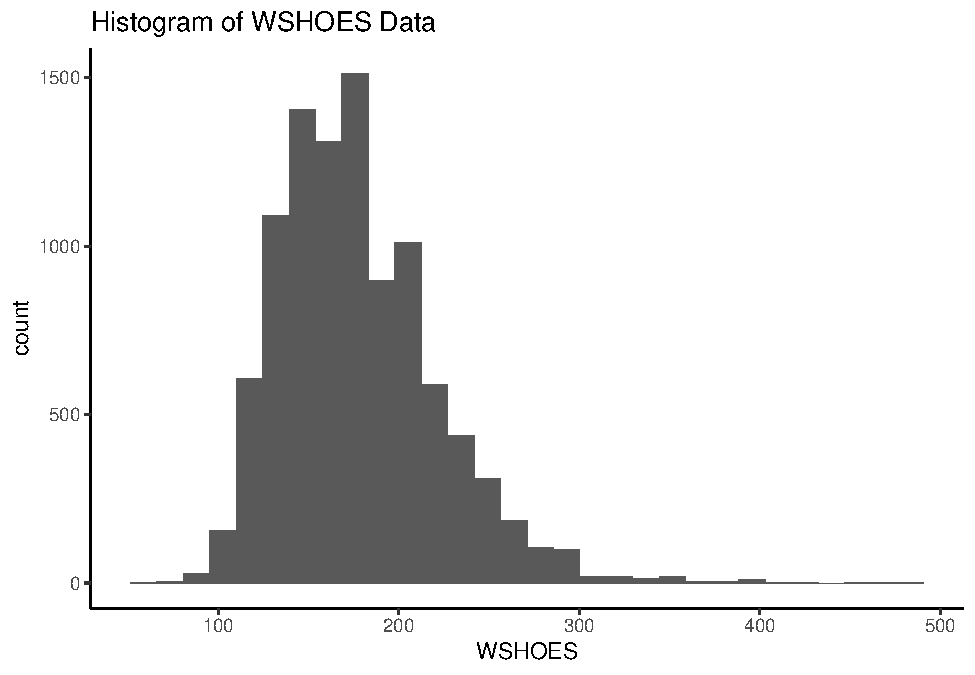
\includegraphics{assignment2_files/figure-latex/q7-1.pdf}

\begin{Shaded}
\begin{Highlighting}[]
\KeywordTok{ggplot}\NormalTok{(hs15, }\KeywordTok{aes}\NormalTok{(}\DataTypeTok{sample =}\NormalTok{ WSHOES)) }\OperatorTok{+}
\StringTok{  }\KeywordTok{geom_qq}\NormalTok{() }\OperatorTok{+}
\StringTok{  }\KeywordTok{geom_qq_line}\NormalTok{() }\OperatorTok{+}
\StringTok{  }\KeywordTok{theme_classic}\NormalTok{() }\OperatorTok{+}
\StringTok{  }\KeywordTok{labs}\NormalTok{(}
    \DataTypeTok{title =} \StringTok{"QQ Plot of WSHOES Data"}
\NormalTok{  )}
\end{Highlighting}
\end{Shaded}

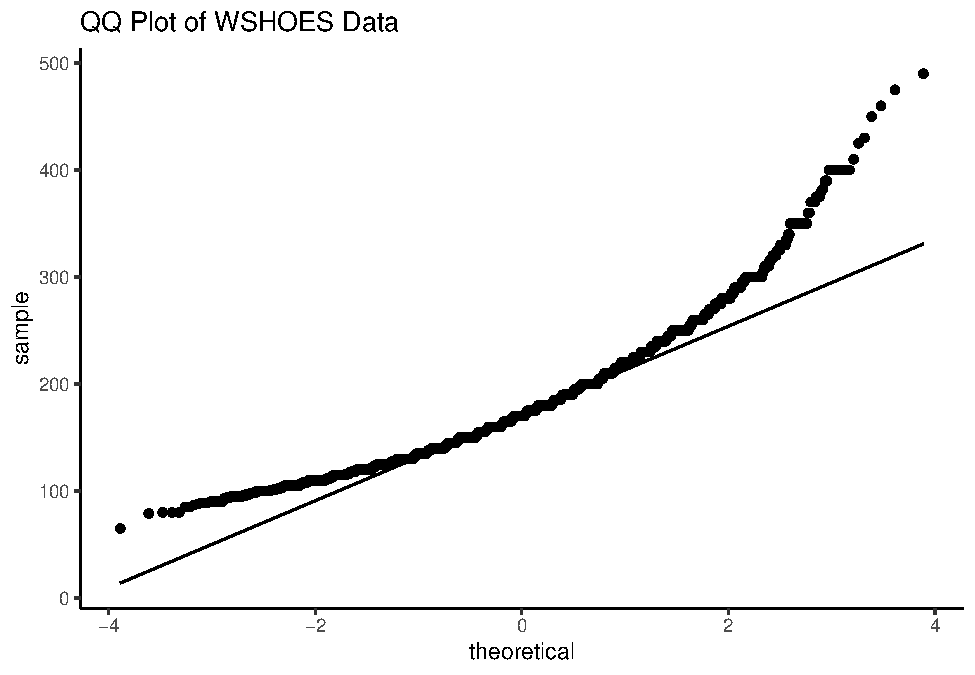
\includegraphics{assignment2_files/figure-latex/q7-2.pdf}

\begin{Shaded}
\begin{Highlighting}[]
\KeywordTok{ggplot}\NormalTok{(hs15, }\KeywordTok{aes}\NormalTok{(}\DataTypeTok{sample =}\NormalTok{ WSHOES)) }\OperatorTok{+}
\StringTok{  }\NormalTok{qqplotr}\OperatorTok{::}\KeywordTok{stat_pp_point}\NormalTok{() }\OperatorTok{+}
\StringTok{  }\NormalTok{qqplotr}\OperatorTok{::}\KeywordTok{stat_pp_band}\NormalTok{() }\OperatorTok{+}
\StringTok{  }\KeywordTok{theme_classic}\NormalTok{() }\OperatorTok{+}
\StringTok{  }\KeywordTok{labs}\NormalTok{(}
    \DataTypeTok{title =} \StringTok{"PP Plot of WSHOES Data"}
\NormalTok{  )}
\end{Highlighting}
\end{Shaded}

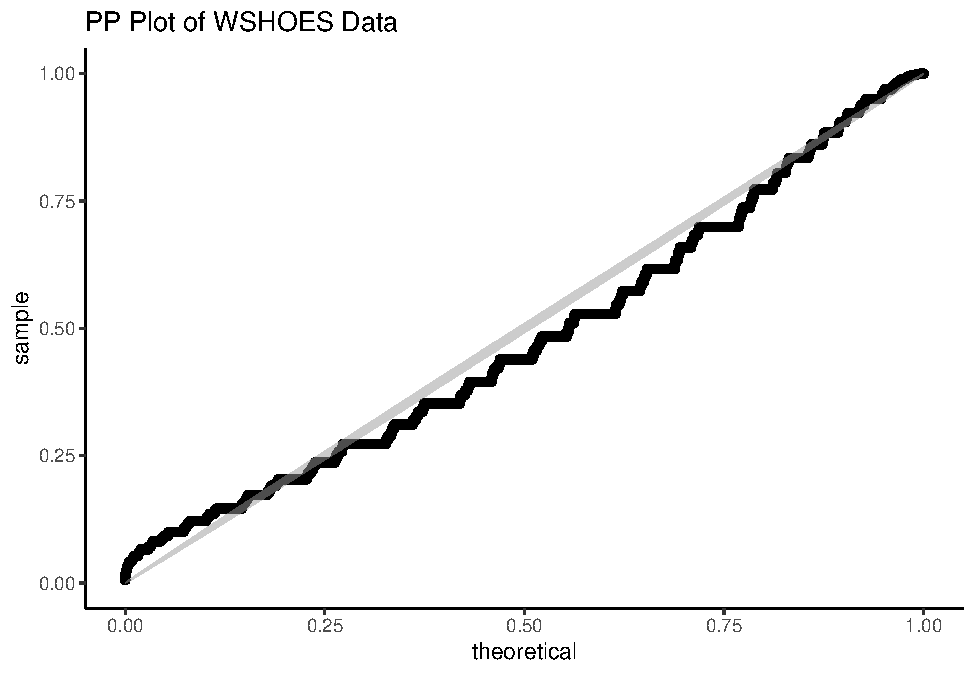
\includegraphics{assignment2_files/figure-latex/q7-3.pdf}

\begin{Shaded}
\begin{Highlighting}[]
\KeywordTok{ggplot}\NormalTok{(hs15, }\KeywordTok{aes}\NormalTok{(}\DataTypeTok{y =}\NormalTok{ WSHOES, }\DataTypeTok{group =} \KeywordTok{as.factor}\NormalTok{(SEX01))) }\OperatorTok{+}
\StringTok{  }\KeywordTok{geom_boxplot}\NormalTok{() }\OperatorTok{+}
\StringTok{  }\KeywordTok{theme_classic}\NormalTok{() }\OperatorTok{+}
\StringTok{  }\KeywordTok{labs}\NormalTok{(}
    \DataTypeTok{title =} \StringTok{"Boxplot of WSHOES by SEX01"}
\NormalTok{  )}
\end{Highlighting}
\end{Shaded}

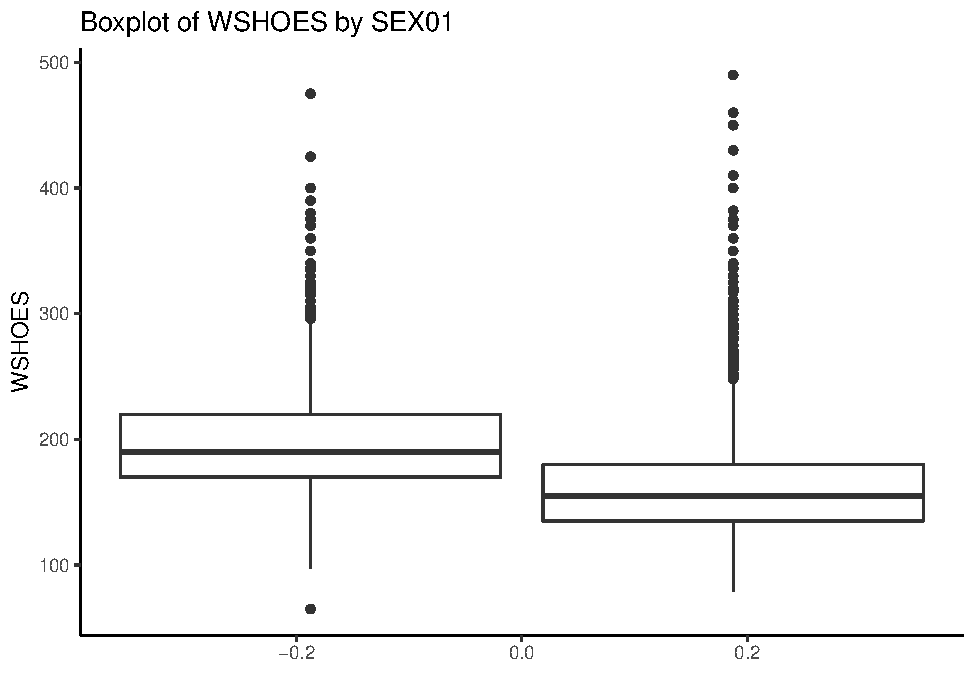
\includegraphics{assignment2_files/figure-latex/q7-4.pdf}

\begin{Shaded}
\begin{Highlighting}[]
\KeywordTok{ggplot}\NormalTok{(hs15, }\KeywordTok{aes}\NormalTok{(}\DataTypeTok{x =}\NormalTok{ BMI, }\DataTypeTok{y =}\NormalTok{ WSHOES)) }\OperatorTok{+}
\StringTok{  }\KeywordTok{geom_jitter}\NormalTok{() }\OperatorTok{+}
\StringTok{  }\KeywordTok{theme_classic}\NormalTok{() }\OperatorTok{+}
\StringTok{  }\KeywordTok{labs}\NormalTok{(}
    \DataTypeTok{title =} \StringTok{"Plot of WSHOES by BMI"}
\NormalTok{  )}
\end{Highlighting}
\end{Shaded}

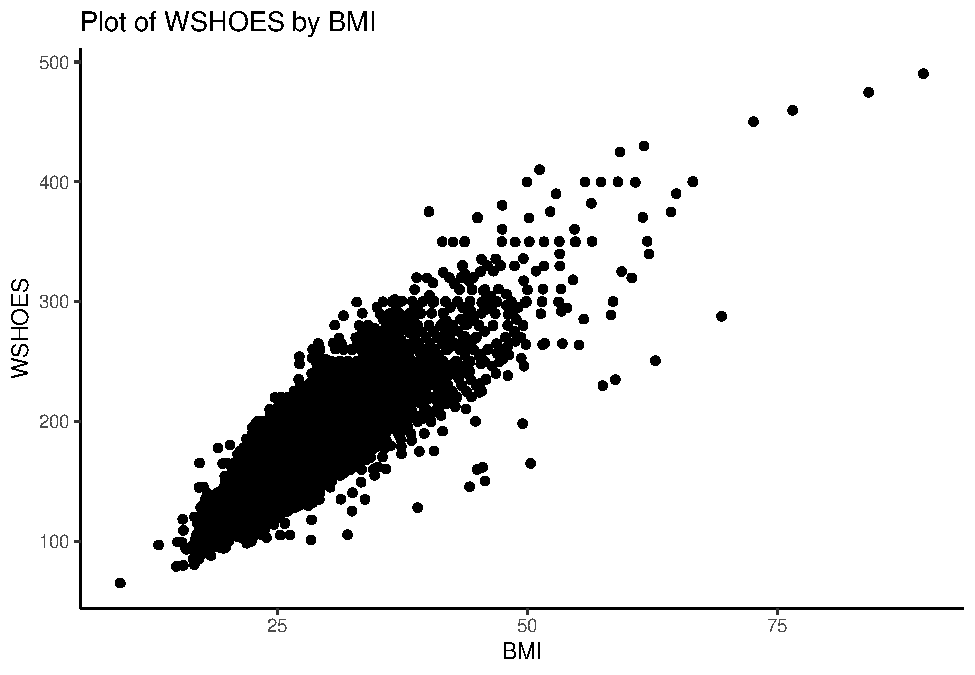
\includegraphics{assignment2_files/figure-latex/q7-5.pdf}

\begin{Shaded}
\begin{Highlighting}[]
\KeywordTok{ggplot}\NormalTok{(hs15, }\KeywordTok{aes}\NormalTok{(}\DataTypeTok{x =}\NormalTok{ BMI, }\DataTypeTok{y =}\NormalTok{ WSHOES, }\DataTypeTok{color =} \KeywordTok{as.factor}\NormalTok{(SEX01))) }\OperatorTok{+}
\StringTok{  }\KeywordTok{geom_jitter}\NormalTok{() }\OperatorTok{+}
\StringTok{  }\KeywordTok{theme_classic}\NormalTok{() }\OperatorTok{+}
\StringTok{  }\KeywordTok{labs}\NormalTok{(}
    \DataTypeTok{title =} \StringTok{"Plot of WSHOES by BMI Colored by SEX01"}
\NormalTok{  )}
\end{Highlighting}
\end{Shaded}

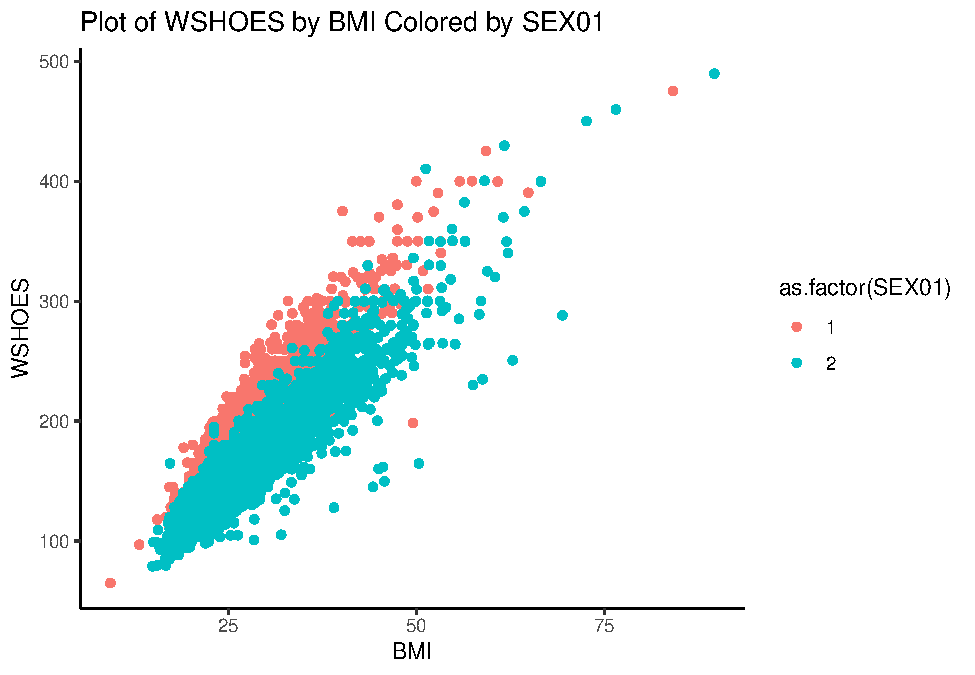
\includegraphics{assignment2_files/figure-latex/q7-6.pdf}

The plots each show how the data is not normally distrubted but is
close. The histogram shows tailing, the qq and pp plots both show how
the data diverage from the normal line.

\hypertarget{run-a-correlation-on-weight-without-shoes-bmi-and-age}{%
\subsection{8. Run a correlation on weight without shoes, BMI, and
age}\label{run-a-correlation-on-weight-without-shoes-bmi-and-age}}

\begin{Shaded}
\begin{Highlighting}[]
\NormalTok{q8Data <-}\StringTok{ }\NormalTok{hs15 }\OperatorTok\StringTok{ }
\StringTok{  }\KeywordTok{select}\NormalTok{(WSHOES, BMI, RESPAGE) }\OperatorTok\StringTok{ }
\StringTok{  }\KeywordTok{drop_na}\NormalTok{()}

\KeywordTok{cor}\NormalTok{(q8Data)}
\end{Highlighting}
\end{Shaded}

\begin{verbatim}
##              WSHOES        BMI     RESPAGE
## WSHOES   1.00000000 0.85844185 -0.05209302
## BMI      0.85844185 1.00000000  0.01085119
## RESPAGE -0.05209302 0.01085119  1.00000000
\end{verbatim}

\begin{Shaded}
\begin{Highlighting}[]
\KeywordTok{corrplot}\NormalTok{(}\KeywordTok{cor}\NormalTok{(q8Data), }\DataTypeTok{method =} \StringTok{'ellipse'}\NormalTok{)}
\end{Highlighting}
\end{Shaded}

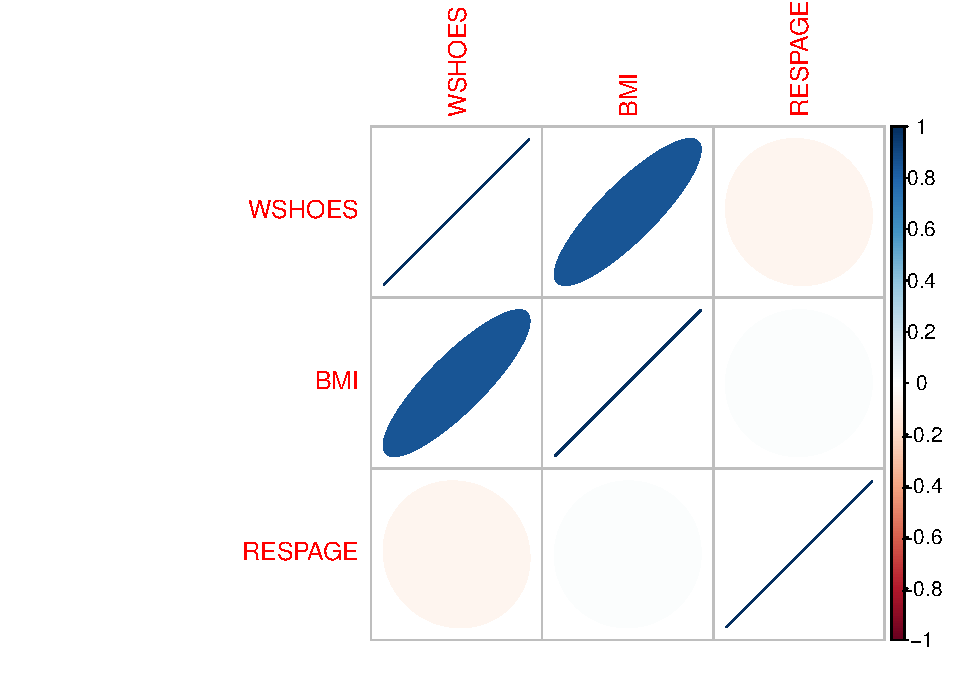
\includegraphics{assignment2_files/figure-latex/q8-1.pdf} As can be
inferred from the plot or taken directly from the matrix, it is clear
there is a strong correlation with BMI and weight without shoes. There
is a very week correlation with weight without shoes and age and no
correlation with BMI and age.


\end{document}
